\documentclass[parskip=full]{scrartcl}

\usepackage[utf8]{inputenc} % use utf8 file encoding for TeX sources
\usepackage[T1]{fontenc} % avoid garbled Unicode text in pdf
\usepackage[german]{babel} % german hyphenation, quotes, etc
\usepackage{hyperref} % detailed hyperlink/pdf configuration
\hypersetup{ % ‘texdoc hyperref‘ for options
pdftitle={Lamb.da - Das Spiel}
}
\usepackage{csquotes} % provides \enquote{} macro for "quotes"
\usepackage{graphicx}
\usepackage{float}
\usepackage{geometry}
\usepackage{enumerate}
\usepackage{titlesec}
\usepackage{mdwlist}
\usepackage{subcaption}
\usepackage{courier}

\newcommand{\sectionbreak}{\clearpage}

\title{Lamb.da - Das Spiel}
\subtitle{Entwurfsdokument}
%\date{October 12, 123}
\author{
Farid El-Haddad,  Florian Fervers,  Kai Fieger,
\\
Robert Hochweiß, Kay Schmitteckert
}

%Header mit KIT-Logo
\titlehead{
	\begin{minipage}{14cm}
		\begin{flushright}
			\vspace{-25mm}
			\hspace{-40mm}
	  	\includegraphics*{kitlogo_de_rgb.pdf} 
		\end{flushright}
  	\end{minipage}
  	\\
	\centerline{\hrulefill} %Linie unterm Logo
}

\begin{document}
	\maketitle
	\begin{center}
	
\includegraphics[width=250pt]{./icon.png}
	\end{center}

	\newpage
	\sloppy
	\tableofcontents
	\fussy
	\newpage
	\section{Einleitung}

Die Applikation "`Lambd.da"' soll Kindern im Grundschulalter auf eine spielerische Art und Weise die wesentlichen Aspekte des untypisierten Lambda-Kalküls und damit auch die Grundlage der funktionalen Programmierung vermitteln. In unserer Entwurfsdokumentation beschreiben und modellieren wir unsere Entwurfsentscheidungen und präsentieren dabei auch die Softwarearchitektur unserer Applikation.

Zunächst beschreiben wir die Funktionen der Applikation, die sich während der Entwurfsphase erst herauskristallisiert haben und deshalb noch nicht im Pflichtenheft erwähnt wurden. Anschließend wird erwähnt, welche der im Pflichtenheft genannten Wunschkriterien nicht mehr umgesetzt werden, da sich bereits in der Entwurfsphase ergab, dass wir diese aus diversen Gründen nicht umsetzen können.

Im Kapitel Grobentwurf erläutern wir dann die von uns gewählten Designentscheidungen wie beispielsweise die eingesetzten Entwurfsmusters und beschreiben die Grobstruktur unserer Klassenpakete. Der Hauptteil und dabei auch der umfassendste Teil unseres Entwurfsdokuments bildet jedoch das Kapitel Feinentwurf mit unserer Klassendokumentation, in der alle Klassen und deren Methoden sowie deren Attribute und mögliche auftretende Exceptions aufgelistet und beschrieben werden. Es werden auch unsere eigenen, verwendeten Interfaces beschrieben. Passend dazu fügen wir noch UML-Klassendiagramme zu diesem Entwurfsdokument an, in denen unsere beschriebenen Klassen und deren Komponenten als auch die Beziehungen zwischen den Klassen modelliert werden.

Des Weiteren Erläutern wir im Kapitel Datenstrukturen, wie die dauerhaft zu speichernden, logischen Komponenten unserer Applikation gespeichert und verwaltet und unsere Assets wie die Level des Spiels geladen werden. Wichtige Programmabläufe und die daraus resultierende Interaktion der Klassen untereinander werden durch UML-Sequenzdiagramme im Kapitel dynamische Diagramme beschrieben.
	\newpage
	\section{Grobentwurf}

\subsection{\texttt{libGDX}}
%kann auch gelöscht werden wenn jemand was Besseres einfällt
libGDX ist ein Framework allein für die Spieleentwicklung und wurde gewählt um die Entwicklung des Produkts zu vereinfachen.
Viele von uns benötigte Funktionalitäten sind in libGDX schon mit inbegriffen, wodurch wir erheblich Arbeit einsparen.
Dabei wird es zum Beispiel besonders einfach gemacht die Benutzeroberfläche oder Animationen zu erstellen.
Zusätzlich soll das Produkt auf mehreren Plattformen laufen. libGDX erlaubt es uns möglichst plattformneutral zu entwickeln 
und relativ einfach entsprechende, spezialisierte Programmversionen zu erstellen.

\subsection{\texttt{Model-View-Controller}}

\subsection{\texttt{Observer}}

\subsection{\texttt{Visitor}}

\subsection{\texttt{Singleton-Pattern}}
Da wir verschiedene Klassen benötigen von denen es aber nur ein Objekt geben soll und ein globaler sowie einfacher Zugriff auf diese Objekte geben soll, bietet sich das Singleton-Pattern natürlich besonders an. So gibt es beispielsweise die Klasse $\texttt{AssetModel}$, welche alle benötigten Ressourcen für die Applikation enthält und von mehreren Klassen gleichzeitig benutzt wird.


\subsection{\texttt{Strategy}}

	\newpage
	\section{Feinentwurf}

\subsection{\texttt{package lambda}}

\subsubsection{\normalfont \texttt{public class \textbf{Observable}<Observer>}}

\begin{description}
\item[Beschreibung] \hfill \\ Repräsentiert ein Objekt, das von Beobachtern überwacht werden kann. Dabei informiert das Objekt alle Beobachter, sobald Änderungen an ihm vorgenommen werden.

\item[Typ-Parameter] \hfill \\
	\vspace{-.8cm}
	\begin{itemize}
		\item $\texttt{<Observer>}$ \\ Der Typ eines Beobachters.
	\end{itemize}

\item[Attribute] \hfill \\
	\vspace{-.8cm}
	\begin{itemize}
		\item $\texttt{private List<Observer> \textbf{observers}}$ \\ Die Liste der Beobachter dieses Objektes.
	\end{itemize}
	
\item[Konstruktoren] \hfill \\
	\vspace{-.8cm}
	\begin{itemize}
		\item $\texttt{public \textbf{Observable}()}$ \\ Instanziiert ein Objekt dieser Klasse.
	\end{itemize}
	
\item[Methoden] \hfill \\
	\vspace{-.8cm}
	\begin{itemize}
		\item $\texttt{public void \textbf{addObserver}(Observer o)}$ \\ Fügt den gegebenen Beobachter diesem Objekt hinzu, sodass dieser bei Änderungen informiert wird.
		\begin{description}
			\item[Parameter] \hfill \\
			\vspace{-.8cm}
			\begin{itemize}
				\item $\texttt{Observer o}$ \\ Der neue Beobachter.
			\end{itemize}
			\item[Exceptions] \hfill \\
			\vspace{-.8cm}
			\begin{itemize}
				\item $\texttt{NullPointerException}$ \\ Falls $\texttt{o == null}$ ist.
			\end{itemize}
		\end{description}
		
		\item $\texttt{public void \textbf{removeObserver}(Observer o)}$ \\ Entfernt den Beobachter aus der Liste, falls dieser darin existiert, sodass dieser nicht mehr bei Änderungen informiert wird.
		\begin{description}
			\item[Parameter] \hfill \\
			\vspace{-.8cm}
			\begin{itemize}
				\item $\texttt{Observer o}$ \\ Der zu entfernende Beobachter.
			\end{itemize}
			\item[Exceptions] \hfill \\
			\vspace{-.8cm}
			\begin{itemize}
				\item $\texttt{NullPointerException}$ \\ Falls $\texttt{o == null}$ ist.
			\end{itemize}
		\end{description}
		
		\item $\texttt{public void \textbf{notify}(Consumer<Observer> notifier)}$ \\ Ruft die gegebene Funktion auf allen Beobachtern auf. Wird benutzt, um Beobachter über Änderungen am Objekt zu informieren.
		\begin{description}
			\item[Parameter] \hfill \\
			\vspace{-.8cm}
			\begin{itemize}
				\item $\texttt{Consumer<Observer> notifier}$ \\ Die Funktion, die auf allen Beobachtern ausgeführt wird.
			\end{itemize}
			\item[Exceptions] \hfill \\
			\vspace{-.8cm}
			\begin{itemize}
				\item $\texttt{NullPointerException}$ \\ Falls $\texttt{notifier == null}$ ist.
			\end{itemize}
		\end{description}
	\end{itemize}
\end{description}

\subsection{\texttt{package lambda.model.lambdaterm}}

\subsubsection{\normalfont \texttt{public abstract class \textbf{LambdaTerm} }}

\begin{description}
\item[Beschreibung] \hfill \\ Repräsentiert einen Term im Lambda-Kalkül bzw. ein Knoten in der Baumstruktur eines Lambda-Terms.

\item[Attribute] \hfill \\
	\vspace{-.8cm}
	\begin{itemize}
		\item $\texttt{private LambdaTerm \textbf{parent}}$ \\ Der Elternknoten dieses Terms. Kann auch $\texttt{null}$ sein, falls der Knoten eine Wurzel ist.
		\item $\texttt{private boolean \textbf{locked}}$ \\ Gibt an, ob dieser Knoten im Editor verändert werden kann.
	\end{itemize}
	
\item[Konstruktoren] \hfill \\
	\vspace{-.8cm}
	\begin{itemize}
		\item $\texttt{public \textbf{LambdaTerm}(LambdaTerm parent, boolean locked)}$ \\ Instanziiert ein Objekt dieser Klasse mit dem gegebenen Elternknoten.
		\begin{description}
			\item[Parameter] \hfill \\
			\vspace{-.8cm}
			\begin{itemize}
				\item $\texttt{LambdaTerm parent}$ \\ Der Elternknoten dieses Terms. Kann auch $\texttt{null}$ sein, falls der Knoten eine Wurzel ist.
				\item $\texttt{boolean locked}$ \\ Gibt an, ob dieser Knoten im Editor verändert werden kann.
			\end{itemize}
		\end{description}
	\end{itemize}
	
\item[Methoden] \hfill \\
	\vspace{-.8cm}
	\begin{itemize}
		\item $\texttt{public abstract <T> T \textbf{accept}(LambdaTermVisitor<T> visitor)}$ \\ Nimmt den gegebenen Besucher entgegen und ruft dessen $\texttt{visit}$-Methode auf. Die Rückgabe des Besuchers wird auch von dieser Methode zurückgegeben.
		\begin{description}
			\item[Typ-Parameter] \hfill \\
				\vspace{-.8cm}
				\begin{itemize}
					\item $\texttt{<T>}$ \\ Der Typ des Rückgabewertes des Besuchers. Wird benötigt, um verschiedene Rückgabewerte von verschiedenen Besucherklassen zu ermöglichen.
				\end{itemize}
			\item[Parameter] \hfill \\
			\vspace{-.8cm}
			\begin{itemize}
				\item $\texttt{LambdaTermVisitor<T> visitor}$ \\ Der Besucher, der entgegen genommen wird.
			\end{itemize}
			\item[Rückgabe] \hfill \\
			\vspace{-.8cm}
			\begin{itemize}
				\item Gibt den Rückgabewert des Besuchers zurück.
			\end{itemize}
			\item[Exceptions] \hfill \\
			\vspace{-.8cm}
			\begin{itemize}
				\item $\texttt{NullPointerException}$ \\ Falls $\texttt{visitor == null}$ ist.
			\end{itemize}
		\end{description}
		
		\item $\texttt{public void \textbf{notifyRoot}(Consumer<LambdaTermObserver> notifier)}$ \\ Gibt die Nachricht weiter zur Wurzel, wo die Beobachter informiert werden.
		\begin{description}
			\item[Parameter] \hfill \\
			\vspace{-.8cm}
			\begin{itemize}
				\item $\texttt{Consumer<LambdaTermObserver> notifier}$ \\ Die Funktion, die auf allen Beobachtern ausgeführt wird.
			\end{itemize}
			\item[Exceptions] \hfill \\
			\vspace{-.8cm}
			\begin{itemize}
				\item $\texttt{NullPointerException}$ \\ Falls $\texttt{notifier == null}$ ist.
			\end{itemize}
		\end{description}
		
		\item $\texttt{public boolean \textbf{isValue}()}$ \\ Gibt zurück, ob dieser Term ein Wert - d.h. eine Abstraktion oder Variable - ist. Gibt in der Standard-Implementierung $\texttt{false}$ zurück und wird von entsprechenden Unterklassen überschrieben.
		\begin{description}
			\item[Rückgabe] \hfill \\
			\vspace{-.8cm}
			\begin{itemize}
				\item Gibt zurück, ob dieser Term ein Wert ist.
			\end{itemize}
		\end{description}
		
		\item $\texttt{public LambdaTerm \textbf{getParent}()}$ \\ Gibt den Elternknoten dieses Knotens wieder oder $\texttt{null}$, falls dieser Knoten eine Wurzel ist.
		\begin{description}
			\item[Rückgabe] \hfill \\
			\vspace{-.8cm}
			\begin{itemize}
				\item Der Elternknoten dieses Knotens.
			\end{itemize}
		\end{description}
		
		\item $\texttt{public boolean \textbf{isLocked}()}$ \\ Gibt zurück, ob dieser Knoten im Editor verändert werden kann.
		\begin{description}
			\item[Rückgabe] \hfill \\
			\vspace{-.8cm}
			\begin{itemize}
				\item Gibt zurück, ob dieser Knoten im Editor verändert werden kann.
			\end{itemize}
		\end{description}
		
		\item $\texttt{public boolean \textbf{equals}(Object o)}$ \\ Gibt zurück, ob dieses und das gegebene Element gleich sind.
		\begin{description}
			\item[Rückgabe] \hfill \\
			\vspace{-.8cm}
			\begin{itemize}
				\item Gibt zurück, ob dieses und das gegebene Element gleich sind.
			\end{itemize}
		\end{description}
	\end{itemize}
\end{description}

\subsubsection{\normalfont \texttt{public interface \textbf{LambdaTermObserver}}}

\begin{description}
\item[Beschreibung] \hfill \\ Repräsentiert einen Beobachter eines Lambda-Terms, welcher über Änderungen am Term informiert wird.

\item[Methoden] \hfill \\
	\vspace{-.8cm}
	\begin{itemize}
		\item $\texttt{public void \textbf{replaceTerm}(LambdaTerm old, LambdaTerm new)}$ \\ Wird aufgerufen um dem Beobachter mitzuteilen, dass der gegebene alte Term durch den gegebenen neuen ersetzt wird. Einer von beiden Parametern kann $\texttt{null}$ sein, niemals aber beide.
		\begin{description}
			\item[Parameter] \hfill \\
			\vspace{-.8cm}
			\begin{itemize}
				\item $\texttt{LambdaTerm old}$ \\ Der ersetzte Term.
				\item $\texttt{LambdaTerm new}$ \\ Der neue Term.
			\end{itemize}
		\end{description}
		
		\item $\texttt{public void \textbf{setColor}(LambdaValue term, Color color)}$ \\ Wird aufgerufen um dem Beobachter mitzuteilen, dass die Farbe des gegebenen Terms durch die gegebene neue Farbe ersetzt wird.
		\begin{description}
			\item[Parameter] \hfill \\
			\vspace{-.8cm}
			\begin{itemize}
				\item $\texttt{LambdaValue term}$ \\ Der veränderte Term.
				\item $\texttt{Color color}$ \\ Die neue Farbe des Terms.
			\end{itemize}
		\end{description}
	\end{itemize}
\end{description}

\subsubsection{\normalfont \texttt{public class \textbf{LambdaApplication} extends LambdaTerm}}

\begin{description}
\item[Beschreibung] \hfill \\ Repräsentiert eine Applikation im Lambda-Kalkül.
\item[Attribute] \hfill \\
	\vspace{-.8cm}
	\begin{itemize}
		\item $\texttt{private LambdaTerm \textbf{first}}$ \\ Linker bzw. erster Kindknoten der Applikation.
		\item $\texttt{private LambdaTerm \textbf{second}}$ \\ Rechter bzw. zweiter Kindknoten der Applikation.
	\end{itemize}
	
\item[Konstruktoren] \hfill \\
	\vspace{-.8cm}
	\begin{itemize}
		\item $\texttt{public \textbf{LambdaApplication}(LambdaTerm parent, boolean locked)}$ \\ Instanziiert ein Objekt dieser Klasse mit dem gegebenen Elternknoten.
		\begin{description}
			\item[Parameter] \hfill \\
			\vspace{-.8cm}
			\begin{itemize}
				\item $\texttt{LambdaTerm parent}$ \\ Der Elternknoten dieses Terms. $\texttt{null}$ ist erlaubt, resultiert aber in einem ungültigen Lambda-Term.
				\item $\texttt{boolean locked}$ \\ Gibt an, ob dieser Knoten im Editor verändert werden kann.
			\end{itemize}
		\end{description}
	\end{itemize}
	
\item[Methoden] \hfill \\
	\vspace{-.8cm}
	\begin{itemize}
		\item $\texttt{public <T> T \textbf{accept}(LambdaTermVisitor<T> visitor)}$ \\ Siehe $\texttt{LambdaTerm.accept}$
		
		\item $\texttt{public void \textbf{setFirst}(LambdaTerm first)}$ \\ Setzt den linken bzw. ersten Kindknoten dieser Applikation und informiert alle Beobachter über diese Änderung.
		\begin{description}
			\item[Parameter] \hfill \\
			\vspace{-.8cm}
			\begin{itemize}
				\item $\texttt{LambdaTerm first}$ \\ Der neue linke Kindknoten. $\texttt{null}$ ist erlaubt, resultiert aber in einem ungültigen Lambda-Term.
			\end{itemize}
		\end{description}
		
		\item $\texttt{public LambdaTerm \textbf{getFirst}()}$ \\ Gibt den linken bzw. ersten Kindknoten dieser Applikation zurück.
		\begin{description}
			\item[Rückgabe] \hfill \\
			\vspace{-.8cm}
			\begin{itemize}
				\item  Der linke Kindknoten dieser Applikation.
			\end{itemize}
		\end{description}
		
		\item $\texttt{public void \textbf{setSecond}(LambdaTerm second)}$ \\ Setzt den rechten bzw. zweiten Kindknoten dieser Applikation und informiert alle Beobachter über diese Änderung.
		\begin{description}
			\item[Parameter] \hfill \\
			\vspace{-.8cm}
			\begin{itemize}
				\item $\texttt{LambdaTerm second}$ \\ Der neue rechte Kindknoten. $\texttt{null}$ ist erlaubt, resultiert aber in einem ungültigen Lambda-Term.
			\end{itemize}
		\end{description}
		
		\item $\texttt{public LambdaTerm \textbf{getSecond}()}$ \\ Gibt den rechten bzw. zweiten Kindknoten dieser Applikation zurück.
		\begin{description}
			\item[Rückgabe] \hfill \\
			\vspace{-.8cm}
			\begin{itemize}
				\item  Der rechte Kindknoten dieser Applikation.
			\end{itemize}
		\end{description}
		
		\item $\texttt{public boolean \textbf{equals}(Object o)}$ \\ Gibt zurück, ob dieses und das gegebene Element gleich sind. Zwei Applikationen sind gleich, wenn beide rechte Kindknoten gleich und beide linke Kindknoten gleich sind.
		\begin{description}
			\item[Rückgabe] \hfill \\
			\vspace{-.8cm}
			\begin{itemize}
				\item Gibt zurück, ob dieses und das gegebene Element gleich sind.
			\end{itemize}
		\end{description}
	\end{itemize}
\end{description}

\subsubsection{\normalfont \texttt{public abstract class \textbf{LambdaValue} extends LambdaTerm}}

\begin{description}
\item[Beschreibung] \hfill \\ Repräsentiert einen Wert - d.h. Abstraktion oder Variable - im Lambda-Kalkül.
\item[Attribute] \hfill \\
	\vspace{-.8cm}
	\begin{itemize}
		\item $\texttt{private Color \textbf{color}}$ \\ Die Farbe dieses Wertes, äquivalent zum Variablennamen.
	\end{itemize}
	
\item[Konstruktoren] \hfill \\
	\vspace{-.8cm}
	\begin{itemize}
		\item $\texttt{public \textbf{LambdaValue}(LambdaTerm parent, Color color, boolean locked)}$ \\ Instanziiert ein Objekt dieser Klasse mit dem gegebenen Elternknoten und der gegebenen Farbe.
		\begin{description}
			\item[Parameter] \hfill \\
			\vspace{-.8cm}
			\begin{itemize}
				\item $\texttt{LambdaTerm parent}$ \\ Der Elternknoten dieses Terms. $\texttt{null}$ ist erlaubt, falls der Term eine Wurzel ist.
				\item $\texttt{Color color}$ \\ Die Farbe dieses Wertes.
				\item $\texttt{boolean locked}$ \\ Gibt an, ob dieser Knoten im Editor verändert werden kann.
			\end{itemize}
			\item[Exceptions] \hfill \\
			\vspace{-.8cm}
			\begin{itemize}
				\item $\texttt{NullPointerException}$ \\ Falls $\texttt{color == null}$ ist.
			\end{itemize}
		\end{description}
	\end{itemize}
	
\item[Methoden] \hfill \\
	\vspace{-.8cm}
	\begin{itemize}
		\item $\texttt{public boolean \textbf{isValue}()}$ \\ Gibt zurück, ob dieser Term ein Wert ist. Überschreibt die Funktion in $\texttt{LambdaTerm}$ und gibt hier immer $\texttt{true}$ zurück.
		\begin{description}
			\item[Rückgabe] \hfill \\
			\vspace{-.8cm}
			\begin{itemize}
				\item Gibt zurück, ob dieser Term ein Wert ist.
			\end{itemize}
		\end{description}
		
		\item $\texttt{public void \textbf{setColor}(Color color)}$ \\ Setzt die Farbe dieses Wertes und informiert alle Beobachter über diese Änderung.
		\begin{description}
			\item[Parameter] \hfill \\
			\vspace{-.8cm}
			\begin{itemize}
				\item $\texttt{Color color}$ \\ Die neue Farbe.
			\end{itemize}
			\item[Exceptions] \hfill \\
			\vspace{-.8cm}
			\begin{itemize}
				\item $\texttt{NullPointerException}$ \\ Falls $\texttt{color == null}$ ist.
			\end{itemize}
		\end{description}
		
		\item $\texttt{public Color \textbf{getColor}()}$ \\ Gibt die Farbe dieses Wertes zurück.
		\begin{description}
			\item[Rückgabe] \hfill \\
			\vspace{-.8cm}
			\begin{itemize}
				\item Die Farbe dieses Wertes.
			\end{itemize}
		\end{description}
	\end{itemize}
\end{description}

\subsubsection{\normalfont \texttt{public class \textbf{LambdaAbstraction} extends LambdaValue}}

\begin{description}
\item[Beschreibung] \hfill \\ Repräsentiert eine Abstraktion im Lambda-Kalkül.
\item[Attribute] \hfill \\
	\vspace{-.8cm}
	\begin{itemize}
		\item $\texttt{private LambdaTerm \textbf{inside}}$ \\ Der Term innerhalb der Applikation. Kann $\texttt{null}$ sein, resultiert aber in einem ungültigen Term.
	\end{itemize}
	
\item[Konstruktoren] \hfill \\
	\vspace{-.8cm}
	\begin{itemize}
		\item $\texttt{public \textbf{LambdaAbstraction}(LambdaTerm parent, Color color, boolean locked)}$ \\ Instanziiert ein Objekt dieser Klasse mit dem gegebenen Elternknoten und der gegebenen Farbe.
		\begin{description}
			\item[Parameter] \hfill \\
			\vspace{-.8cm}
			\begin{itemize}
				\item $\texttt{LambdaTerm parent}$ \\ Der Elternknoten dieses Terms. Kann $\texttt{null}$ sein, falls der Term eine Wurzel ist.
				\item $\texttt{Color color}$ \\ Die Farbe der in dieser Abstraktion gebundenen Variable.
				\item $\texttt{boolean locked}$ \\ Gibt an, ob dieser Knoten im Editor verändert werden kann.
			\end{itemize}
			\item[Exceptions] \hfill \\
			\vspace{-.8cm}
			\begin{itemize}
				\item $\texttt{NullPointerException}$ \\ Falls $\texttt{color == null}$ ist.
			\end{itemize}
		\end{description}
	\end{itemize}
	
\item[Methoden] \hfill \\
	\vspace{-.8cm}
	\begin{itemize}
		\item $\texttt{public <T> T \textbf{accept}(LambdaTermVisitor<T> visitor)}$ \\ Siehe $\texttt{LambdaTerm.accept}$
		
		\item $\texttt{public void \textbf{setInside}(LambdaTerm inside)}$ \\ Setzt den Term innerhalb der Abstraktion und informiert alle Beobachter über diese Änderung.
		\begin{description}
			\item[Parameter] \hfill \\
			\vspace{-.8cm}
			\begin{itemize}
				\item $\texttt{LambdaTerm inside}$ \\ Der neue innere Term. Kann $\texttt{null}$ sein, resultiert aber in einem ungültigen Term.
			\end{itemize}
		\end{description}
		
		\item $\texttt{public LambdaTerm \textbf{getInside}()}$ \\ Gibt den Term innerhalb der Abstraktion zurück.
		\begin{description}
			\item[Rückgabe] \hfill \\
			\vspace{-.8cm}
			\begin{itemize}
				\item Der innere Term.
			\end{itemize}
		\end{description}
		
		\item $\texttt{public boolean \textbf{equals}(Object o)}$ \\ Gibt zurück, ob dieses und das gegebene Element gleich sind. Zwei Abstraktionen sind gleich, wenn beide dieselbe Farbe haben und die Kindknoten gleich sind.
		\begin{description}
			\item[Rückgabe] \hfill \\
			\vspace{-.8cm}
			\begin{itemize}
				\item Gibt zurück, ob dieses und das gegebene Element gleich sind.
			\end{itemize}
		\end{description}
	\end{itemize}
\end{description}

\subsubsection{\normalfont \texttt{public class \textbf{LambdaVariable} extends LambdaValue}}

\begin{description}
\item[Beschreibung] \hfill \\ Repräsentiert eine Variable im Lambda-Kalkül.

\item[Konstruktoren] \hfill \\
	\vspace{-.8cm}
	\begin{itemize}
		\item $\texttt{public \textbf{LambdaVariable}(LambdaTerm parent, Color color, boolean locked)}$ \\ Instanziiert ein Objekt dieser Klasse mit dem gegebenen Elternknoten und der gegebenen Farbe.
		\begin{description}
			\item[Parameter] \hfill \\
			\vspace{-.8cm}
			\begin{itemize}
				\item $\texttt{LambdaTerm parent}$ \\ Der Elternknoten dieses Terms. Kann $\texttt{null}$ sein, falls der Term eine Wurzel ist.
				\item $\texttt{Color color}$ \\ Die Farbe der Variable.
				\item $\texttt{boolean locked}$ \\ Gibt an, ob dieser Knoten im Editor verändert werden kann.
			\end{itemize}
			\item[Exceptions] \hfill \\
			\vspace{-.8cm}
			\begin{itemize}
				\item $\texttt{NullPointerException}$ \\ Falls $\texttt{color == null}$ ist.
			\end{itemize}
		\end{description}
	\end{itemize}
	
\item[Methoden] \hfill \\
	\vspace{-.8cm}
	\begin{itemize}
		\item $\texttt{public <T> T \textbf{accept}(LambdaTermVisitor<T> visitor)}$ \\ Siehe $\texttt{LambdaTerm.accept}$
	\end{itemize}
	
	\item $\texttt{public boolean \textbf{equals}(Object o)}$ \\ Gibt zurück, ob dieses und das gegebene Element gleich sind. Zwei Variablen sind gleich, wenn beide dieselbe Farbe haben.
	\begin{description}
		\item[Rückgabe] \hfill \\
		\vspace{-.8cm}
		\begin{itemize}
			\item Gibt zurück, ob dieses und das gegebene Element gleich sind.
		\end{itemize}
	\end{description}
\end{description}

\subsubsection{\normalfont \texttt{public class \textbf{LambdaRoot} extends LambdaTerm implements Observable<LambdaTermObserver>}}

\begin{description}
\item[Beschreibung] \hfill \\ Repräsentiert die Wurzel eines Lambda-Terms. Die Wurzel eines gültigen Terms muss immer eine Instanz dieser Klasse sein.

\item[Attribute] \hfill \\
	\vspace{-.8cm}
	\begin{itemize}
		\item $\texttt{private LambdaTerm \textbf{child}}$ \\ Kind der Wurzel der Applikation.
	\end{itemize}
	
\item[Konstruktoren] \hfill \\
	\vspace{-.8cm}
	\begin{itemize}
		\item $\texttt{public \textbf{LambdaRoot}()}$ \\ Instanziiert ein Objekt dieser Klasse ohne Elternknoten.
	\end{itemize}
	
\item[Methoden] \hfill \\
	\vspace{-.8cm}
	\begin{itemize}
		\item $\texttt{public <T> T \textbf{accept}(LambdaTermVisitor<T> visitor)}$ \\ Siehe $\texttt{LambdaTerm.accept}$
		
		\item $\texttt{public void \textbf{notifyRoot}(Consumer<LambdaTermObserver> notifier)}$ \\ Überschreibt die Funktion von $\texttt{LambdaTerm}$, um die Nachricht vom Kindknoten entgegenzunehmen und $\texttt{notify}$ damit aufzurufen.
		\begin{description}
			\item[Parameter] \hfill \\
			\vspace{-.8cm}
			\begin{itemize}
				\item $\texttt{Consumer<LambdaTermObserver> notifier}$ \\ Die Funktion, die auf allen Beobachtern ausgeführt wird.
			\end{itemize}
			\item[Exceptions] \hfill \\
			\vspace{-.8cm}
			\begin{itemize}
				\item $\texttt{NullPointerException}$ \\ Falls $\texttt{notifier == null}$ ist.
			\end{itemize}
		\end{description}
		
		\item $\texttt{public void \textbf{setChild}(LambdaTerm child)}$ \\ Setzt den  Kindknoten dieser Wurzel und informiert alle Beobachter über diese Änderung.
		\begin{description}
			\item[Parameter] \hfill \\
			\vspace{-.8cm}
			\begin{itemize}
				\item $\texttt{LambdaTerm child}$ \\ Der neue Kindknoten. $\texttt{null}$ ist erlaubt, resultiert aber in einem ungültigen Lambda-Term.
			\end{itemize}
		\end{description}
		
		\item $\texttt{public LambdaTerm \textbf{getChild}()}$ \\ Gibt den Kindknoten dieser Wurzel zurück.
		\begin{description}
			\item[Rückgabe] \hfill \\
			\vspace{-.8cm}
			\begin{itemize}
				\item  Der Kindknoten dieser Wurzel.
			\end{itemize}
		\end{description}
		
		\item $\texttt{public boolean \textbf{equals}(Object o)}$ \\ Gibt zurück, ob dieses und das gegebene Element gleich sind. Zwei Wurzeln sind gleich, wenn beide Kindknoten gleich sind.
		\begin{description}
			\item[Rückgabe] \hfill \\
			\vspace{-.8cm}
			\begin{itemize}
				\item Gibt zurück, ob dieses und das gegebene Element gleich sind.
			\end{itemize}
		\end{description}
	\end{itemize}
\end{description}

\subsubsection{\normalfont \texttt{public final class \textbf{LambdaUtils}}}

\begin{description}
\item[Beschreibung] \hfill \\ Liefert statische Methoden zum einfachen Bearbeiten eines Lambda-Terms.

\item[Konstruktoren] \hfill \\
	\vspace{-.8cm}
	\begin{itemize}
		\item $\texttt{private \textbf{LambdaUtils}()}$ \\ Um zu verhindern, dass diese Klasse instanziiert wird.
	\end{itemize}
	
\item[Methoden] \hfill \\
	\vspace{-.8cm}
	\begin{itemize}
		\item $\texttt{public static LambdaRoot \textbf{split}(LambdaTerm term)}$ \\ Entfernt den gegebenen Knoten aus seinem Elternknoten und fügt ihn in eine neue Wurzel des Typs $\texttt{LambdaRoot}$ ein. Gibt die neue Wurzel zurück.
		\begin{description}
			\item[Parameter] \hfill \\
			\vspace{-.8cm}
			\begin{itemize}
				\item $\texttt{LambdaTerm term}$ \\ Der Term, der abgespalten werden soll.
			\end{itemize}
			\item[Rückgabe] \hfill \\
			\vspace{-.8cm}
			\begin{itemize}
				\item Der abgespaltene Term in einer neuen Wurzel.
			\end{itemize}
			\item[Exceptions] \hfill \\
			\vspace{-.8cm}
			\begin{itemize}
				\item $\texttt{NullPointerException}$ \\ Falls $\texttt{term == null}$ ist.
			\end{itemize}
		\end{description}
	\end{itemize}
\end{description}

\subsection{\texttt{package lambda.model.lambdaterm.visitor}}

\subsubsection{\normalfont \texttt{public interface \textbf{LambdaTermVisitor<R>}}}

\begin{description}
\item[Beschreibung] \hfill \\ Repräsentiert einen Besucher auf einer Lambda-Term Baumstruktur. Der Besucher kann Operationen an der Datenstruktur ausführen und hat optional einen Rückgabewert.

\item[Typ-Parameter] \hfill \\
	\vspace{-.8cm}
	\begin{itemize}
		\item $\texttt{<R>}$ \\ Der Typ des Rückgabewertes.
	\end{itemize}

\item[Methoden] \hfill \\
	\vspace{-.8cm}
	\begin{itemize}
		\item $\texttt{public void \textbf{visit}(LambdaRoot node)}$ \\ Besucht die gegebene Wurzel.
		\begin{description}
			\item[Parameter] \hfill \\
			\vspace{-.8cm}
			\begin{itemize}
				\item $\texttt{LambdaRoot node}$ \\ Die besuchte Wurzel. Ist nie $\texttt{null}$.
			\end{itemize}
		\end{description}
			
		\item $\texttt{public void \textbf{visit}(LambdaApplication node)}$ \\ Besucht die gegebene Applikation.
		\begin{description}
			\item[Parameter] \hfill \\
			\vspace{-.8cm}
			\begin{itemize}
				\item $\texttt{LambdaApplication node}$ \\ Die besuchte Applikation. Ist nie $\texttt{null}$.
			\end{itemize}
		\end{description}
		
		\item $\texttt{public void \textbf{visit}(LambdaAbstraction node)}$ \\ Besucht die gegebene Abstraktion.
		\begin{description}
			\item[Parameter] \hfill \\
			\vspace{-.8cm}
			\begin{itemize}
				\item $\texttt{LambdaAbstraction node}$ \\ Die besuchte Abstraktion. Ist nie $\texttt{null}$.
			\end{itemize}
		\end{description}
		
		\item $\texttt{public void \textbf{visit}(LambdaVariable node)}$ \\ Besucht die gegebene Variable.
		\begin{description}
			\item[Parameter] \hfill \\
			\vspace{-.8cm}
			\begin{itemize}
				\item $\texttt{LambdaVariable node}$ \\ Die besuchte Variable. Ist nie $\texttt{null}$.
			\end{itemize}
		\end{description}
		
		\item $\texttt{public R \textbf{getResult}()}$ \\ Gibt das Resultat der Besucheroperation zurück. Wird nur nach einem Besuch ausgeführt. Gibt in der Standard-Implementierung $\texttt{null}$ zurück.
		\begin{description}
			\item[Rückgabe] \hfill \\
			\vspace{-.8cm}
			\begin{itemize}
				\item Das Resultat der Besucheroperation.
			\end{itemize}
		\end{description}
	\end{itemize}
\end{description}

\subsubsection{\normalfont \texttt{public class \textbf{AlphaConversionVisitor} implements LambdaTermVisitor<Object>}}

\begin{description}
\item[Beschreibung] \hfill \\ Repräsentiert einen Besucher auf einer Lambda-Term Baumstruktur, welcher eine Alpha-Konversion auf ihr ausführt.

\item[Attribute] \hfill \\
	\vspace{-.8cm}
	\begin{itemize}
		\item $\texttt{private Color \textbf{old}}$ \\ Die zu ersetzende Farbe.
		\item $\texttt{private Color \textbf{new}}$ \\ Die neue Farbe.
	\end{itemize}

\item[Konstruktoren] \hfill \\
	\vspace{-.8cm}
	\begin{itemize}
		\item $\texttt{public \textbf{AlphaConversionVisitor}(Color old, Color new)}$ \\ Instanziiert ein Objekt dieser Klasse mit der gegebenen ersetzten und ersetzenden Farbe.
		\begin{description}
			\item[Parameter] \hfill \\
			\vspace{-.8cm}
			\begin{itemize}
				\item $\texttt{Color old}$ \\ Die zu ersetzende Farbe.
				\item $\texttt{Color new}$ \\ Die neue Farbe.
			\end{itemize}
		\end{description}
	\end{itemize}

\item[Methoden] \hfill \\
	\vspace{-.8cm}
	\begin{itemize}
		\item $\texttt{public void \textbf{visit}(LambdaRoot node)}$ \\ Besucht die gegebene Wurzel und traversiert wenn möglich weiter zum Kindknoten.
		\begin{description}
			\item[Parameter] \hfill \\
			\vspace{-.8cm}
			\begin{itemize}
				\item $\texttt{LambdaRoot node}$ \\ Die besuchte Wurzel.
			\end{itemize}
		\end{description}
			
		\item $\texttt{public void \textbf{visit}(LambdaApplication node)}$ \\ Besucht die gegebene Applikation und traversiert wenn möglich weiter zu beiden Kindknoten.
		\begin{description}
			\item[Parameter] \hfill \\
			\vspace{-.8cm}
			\begin{itemize}
				\item $\texttt{LambdaApplication node}$ \\ Die besuchte Applikation.
			\end{itemize}
		\end{description}
		
		\item $\texttt{public void \textbf{visit}(LambdaAbstraction node)}$ \\ Besucht die gegebene Abstraktion. Dabei wird die Farbe wenn nötig ersetzt und wenn möglich weiter zum Kindknoten traversiert.
		\begin{description}
			\item[Parameter] \hfill \\
			\vspace{-.8cm}
			\begin{itemize}
				\item $\texttt{LambdaAbstraction node}$ \\ Die besuchte Abstraktion.
			\end{itemize}
		\end{description}
		
		\item $\texttt{public void \textbf{visit}(LambdaVariable node)}$ \\ Besucht die gegebene Variable und ersetzt die Farbe wenn nötig.
		\begin{description}
			\item[Parameter] \hfill \\
			\vspace{-.8cm}
			\begin{itemize}
				\item $\texttt{LambdaVariable node}$ \\ Die besuchte Variable.
			\end{itemize}
		\end{description}
	\end{itemize}
\end{description}

\subsubsection{\normalfont \texttt{public class \textbf{ColorCollectionVisitor} implements LambdaTermVisitor<Set<Color>{}>}}

\begin{description}
\item[Beschreibung] \hfill \\ Repräsentiert einen Besucher auf einer Lambda-Term Baumstruktur, der die Menge der benutzten Farben in diesem Term zurückgibt.

\item[Attribute] \hfill \\
	\vspace{-.8cm}
	\begin{itemize}
		\item $\texttt{private Set<Color> \textbf{result}}$ \\ Die Menge aller benutzten Farben.
	\end{itemize}

\item[Konstruktoren] \hfill \\
	\vspace{-.8cm}
	\begin{itemize}
		\item $\texttt{public \textbf{ColorCollectionVisitor}()}$ \\ Instanziiert ein Objekt dieser Klasse.
	\end{itemize}

\item[Methoden] \hfill \\
	\vspace{-.8cm}
	\begin{itemize}
		\item $\texttt{public void \textbf{visit}(LambdaRoot node)}$ \\ Besucht die gegebene Wurzel und traversiert wenn möglich weiter zum Kindknoten.
		\begin{description}
			\item[Parameter] \hfill \\
			\vspace{-.8cm}
			\begin{itemize}
				\item $\texttt{LambdaRoot node}$ \\ Die besuchte Wurzel.
			\end{itemize}
		\end{description}
				
		\item $\texttt{public void \textbf{visit}(LambdaApplication node)}$ \\ Besucht die gegebene Applikation und traversiert wenn möglich weiter zu beiden Kindknoten.
		\begin{description}
			\item[Parameter] \hfill \\
			\vspace{-.8cm}
			\begin{itemize}
				\item $\texttt{LambdaApplication node}$ \\ Die besuchte Applikation.
			\end{itemize}
		\end{description}
		
		\item $\texttt{public void \textbf{visit}(LambdaAbstraction node)}$ \\ Besucht die gegebene Abstraktion. Dabei wird die Farbe zur Menge hinzugefügt und wenn möglich weiter zum Kindknoten traversiert.
		\begin{description}
			\item[Parameter] \hfill \\
			\vspace{-.8cm}
			\begin{itemize}
				\item $\texttt{LambdaAbstraction node}$ \\ Die besuchte Abstraktion.
			\end{itemize}
		\end{description}
		
		\item $\texttt{public void \textbf{visit}(LambdaVariable node)}$ \\ Besucht die gegebene Variable und fügt die Farbe zur Menge hinzu.
		\begin{description}
			\item[Parameter] \hfill \\
			\vspace{-.8cm}
			\begin{itemize}
				\item $\texttt{LambdaVariable node}$ \\ Die besuchte Variable.
			\end{itemize}
		\end{description}
		
		\item $\texttt{public Set<Color> \textbf{getResult}()}$ \\ Gibt die Menge der Farben zurück, die in dem besuchten Term benutzt werden.
		\begin{description}
			\item[Rückgabe] \hfill \\
			\vspace{-.8cm}
			\begin{itemize}
				\item Die Menge der benutzten Farben.
			\end{itemize}
		\end{description}
	\end{itemize}
\end{description}

\subsubsection{\normalfont \texttt{public class \textbf{IsColorBoundVisitor} implements LambdaTermVisitor<Boolean>}}

\begin{description}
\item[Beschreibung] \hfill \\ Repräsentiert einen Besucher auf einer Lambda-Term Baumstruktur, der zurückgibt, ob eine Variable mit der gegebenen Farbe in diesem Term gebunden ist.

\item[Attribute] \hfill \\
	\vspace{-.8cm}
	\begin{itemize}
		\item $\texttt{private Color \textbf{color}}$ \\ Die zu überprüfende Farbe.
		\item $\texttt{private boolean \textbf{result}}$ \\ Der Rückgabewert des Besuchs.
	\end{itemize}

\item[Konstruktoren] \hfill \\
	\vspace{-.8cm}
	\begin{itemize}
		\item $\texttt{public \textbf{IsColorBoundVisitor}(Color color)}$ \\ Instanziiert ein Objekt dieser Klasse mit der zu überprüfenden Farbe.
		\begin{description}
			\item[Parameter] \hfill \\
			\vspace{-.8cm}
			\begin{itemize}
				\item $\texttt{Color color}$ \\ Die zu überprüfende Farbe.
			\end{itemize}
			\item[Exceptions] \hfill \\
			\vspace{-.8cm}
			\begin{itemize}
				\item $\texttt{NullPointerException}$ \\ Falls $\texttt{color == null}$ ist.
			\end{itemize}
		\end{description}
	\end{itemize}

\item[Methoden] \hfill \\
	\vspace{-.8cm}
	\begin{itemize}
		\item $\texttt{public void \textbf{visit}(LambdaRoot node)}$ \\ Besucht die gegebene Wurzel und beendet die Traversierung hier.
		\begin{description}
			\item[Parameter] \hfill \\
			\vspace{-.8cm}
			\begin{itemize}
				\item $\texttt{LambdaRoot node}$ \\ Die besuchte Wurzel.
			\end{itemize}
		\end{description}
				
		\item $\texttt{public void \textbf{visit}(LambdaApplication node)}$ \\ Besucht die gegebene Applikation und traversiert wenn möglich weiter zum Elternknoten.
		\begin{description}
			\item[Parameter] \hfill \\
			\vspace{-.8cm}
			\begin{itemize}
				\item $\texttt{LambdaApplication node}$ \\ Die besuchte Applikation.
			\end{itemize}
		\end{description}
		
		\item $\texttt{public void \textbf{visit}(LambdaAbstraction node)}$ \\ Besucht die gegebene Abstraktion und überprüft, ob die Farbe hier gebunden ist. Traversiert wenn nötig und möglich weiter zum Elternknoten.
		\begin{description}
			\item[Parameter] \hfill \\
			\vspace{-.8cm}
			\begin{itemize}
				\item $\texttt{LambdaAbstraction node}$ \\ Die besuchte Abstraktion.
			\end{itemize}
		\end{description}
		
		\item $\texttt{public void \textbf{visit}(LambdaVariable node)}$ \\ Besucht die gegebene Variable und traversiert weiter zum Elternknoten.
		\begin{description}
			\item[Parameter] \hfill \\
			\vspace{-.8cm}
			\begin{itemize}
				\item $\texttt{LambdaVariable node}$ \\ Die besuchte Variable.
			\end{itemize}
		\end{description}
		
		\item $\texttt{public Boolean \textbf{getResult}()}$ \\ Gibt zurück, ob die Variable mit der gegebenen Farbe im Term gebunden ist.
		\begin{description}
			\item[Rückgabe] \hfill \\
			\vspace{-.8cm}
			\begin{itemize}
				\item Gibt zurück, ob die Variable mit der gegebenen Farbe gebunden ist.
			\end{itemize}
		\end{description}
	\end{itemize}
\end{description}

\subsubsection{\normalfont \texttt{public class \textbf{ApplicationVisitor} implements LambdaTermVisitor<LambdaTerm>}}

\begin{description}
\item[Beschreibung] \hfill \\ Repräsentiert einen Besucher auf einer Lambda-Term Baumstruktur, welcher eine Applikation ausführt.

\item[Attribute] \hfill \\
	\vspace{-.8cm}
	\begin{itemize}
		\item $\texttt{private Color \textbf{color}}$ \\ Die Farbe der zu ersetzenden Variablen.
		\item $\texttt{private LambdaTerm \textbf{applicant}}$ \\ Das Argument der Applikation.
		\item $\texttt{private LambdaTerm \textbf{result}}$ \\ Der Term nach der Applikation.
		\item $\texttt{private boolean \textbf{hasCheckedAlphaConversion}}$ \\ Initialisiert mit $\texttt{false}$. Speichert, ob bereits überprüft wurde, ob eine Alpha-Konversion vor der Applikation notwendig ist.
	\end{itemize}

\item[Konstruktoren] \hfill \\
	\vspace{-.8cm}
	\begin{itemize}
		\item $\texttt{public \textbf{ApplicationVisitor}(Color color, LambdaTerm applicant)}$ \\ Instanziiert ein Objekt dieser Klasse mit der gegebenen Variablenfarbe und dem gegebenen Argument.
		\begin{description}
			\item[Parameter] \hfill \\
			\vspace{-.8cm}
			\begin{itemize}
				\item $\texttt{Color color}$ \\ Die Farbe der zu ersetzenden Variablen.
				\item $\texttt{LambdaTerm applicant}$ \\ Das Argument der Applikation.
			\end{itemize}
			\item[Exceptions] \hfill \\
			\vspace{-.8cm}
			\begin{itemize}
				\item $\texttt{NullPointerException}$ \\ Falls $\texttt{color == null}$ oder $\texttt{applicant == null}$ ist.
			\end{itemize}
		\end{description}
	\end{itemize}

\item[Methoden] \hfill \\
	\vspace{-.8cm}
	\begin{itemize}
		\item $\texttt{public void \textbf{visit}(LambdaRoot node)}$ \\ Kann nie aufgerufen werden, da der besuchte Knoten keinen Elternknoten hat, von wo aus eine Applikation ausgeführt werden könnte.
		\begin{description}
			\item[Parameter] \hfill \\
			\vspace{-.8cm}
			\begin{itemize}
				\item $\texttt{LambdaRoot node}$ \\ Die besuchte Wurzel.
			\end{itemize}
		\end{description}
				
		\item $\texttt{public void \textbf{visit}(LambdaApplication node)}$ \\ Besucht die gegebene Applikation und traversiert weiter zu beiden Kindknoten. Dabei werden die Kindknoten auf die Rückgabewerte beider Besuche gesetzt. Speichert als Rückgabewert den besuchten Term.
		\begin{description}
			\item[Parameter] \hfill \\
			\vspace{-.8cm}
			\begin{itemize}
				\item $\texttt{LambdaApplication node}$ \\ Die besuchte Applikation.
			\end{itemize}
		\end{description}
		
		\item $\texttt{public void \textbf{visit}(LambdaAbstraction node)}$ \\ Besucht die gegebene Abstraktion und traversiert weiter zum Kindknoten. Dabei wird der Kindknoten auf den Rückgabewert des Besuchs gesetzt. Speichert als Rückgabewert den besuchten Term.
		\begin{description}
			\item[Parameter] \hfill \\
			\vspace{-.8cm}
			\begin{itemize}
				\item $\texttt{LambdaAbstraction node}$ \\ Die besuchte Abstraktion.
			\end{itemize}
		\end{description}
		
		\item $\texttt{public void \textbf{visit}(LambdaVariable node)}$ \\ Besucht die gegebene Variable und speichert wenn nötig als Rückgabewert $\texttt{applicant}$.
		\begin{description}
			\item[Parameter] \hfill \\
			\vspace{-.8cm}
			\begin{itemize}
				\item $\texttt{LambdaVariable node}$ \\ Die besuchte Variable.
			\end{itemize}
		\end{description}
		
		\item $\texttt{public LambdaTerm \textbf{getResult}()}$ \\ Gibt den Term nach der Applikation zurück.
		\begin{description}
			\item[Rückgabe] \hfill \\
			\vspace{-.8cm}
			\begin{itemize}
				\item Der besuchte Term.
			\end{itemize}
		\end{description}
		
		\item $\texttt{private void \textbf{checkAlphaConversion}()}$ \\ Überprüft, ob eine Alpha-Konversion notwendig ist, falls dies noch nicht getan wurde, und führt diese wenn nötig aus. Entfernt danach das Argument der Applikation aus dem LambdaTerm.
	\end{itemize}
\end{description}

\subsubsection{\normalfont \texttt{public class \textbf{CopyVisitor} implements LambdaTermVisitor<LambdaTerm>}}

\begin{description}
\item[Beschreibung] \hfill \\ Repräsentiert einen Besucher auf einer Lambda-Term Baumstruktur, welcher die Datenstruktur kopiert und die Kopie zurückgibt.

\item[Attribute] \hfill \\
	\vspace{-.8cm}
	\begin{itemize}
		\item $\texttt{private LambdaTerm \textbf{result}}$ \\ Die Kopie.
	\end{itemize}

\item[Konstruktoren] \hfill \\
	\vspace{-.8cm}
	\begin{itemize}
		\item $\texttt{public \textbf{CopyVisitor}()}$ \\ Instanziiert ein Objekt dieser Klasse.
	\end{itemize}

\item[Methoden] \hfill \\
	\vspace{-.8cm}
	\begin{itemize}
		\item $\texttt{public void \textbf{visit}(LambdaRoot node)}$ \\ Besucht die gegebene Wurzel und erstellt eine Kopie. Traversiert zum Kindknoten und speichert den Rückgabewert dieses Besuchs im Kindknoten der Kopie.
		\begin{description}
			\item[Parameter] \hfill \\
			\vspace{-.8cm}
			\begin{itemize}
				\item $\texttt{LambdaRoot node}$ \\ Die besuchte Wurzel.
			\end{itemize}
		\end{description}
				
		\item $\texttt{public void \textbf{visit}(LambdaApplication node)}$ \\ Besucht die gegebene Applikation und erstellt eine Kopie. Traversiert zu beiden Kindknoten und speichert die Rückgabewerte dieser Besuche in den Kindknoten der Kopie.
		\begin{description}
			\item[Parameter] \hfill \\
			\vspace{-.8cm}
			\begin{itemize}
				\item $\texttt{LambdaApplication node}$ \\ Die besuchte Applikation.
			\end{itemize}
		\end{description}
		
		\item $\texttt{public void \textbf{visit}(LambdaAbstraction node)}$ \\ Besucht die gegebene Abstraktion und erstellt eine Kopie. Traversiert zum Kindknoten und speichert den Rückgabewert dieses Besuchs im Kindknoten der Kopie.
		\begin{description}
			\item[Parameter] \hfill \\
			\vspace{-.8cm}
			\begin{itemize}
				\item $\texttt{LambdaAbstraction node}$ \\ Die besuchte Abstraktion.
			\end{itemize}
		\end{description}
		
		\item $\texttt{public void \textbf{visit}(LambdaVariable node)}$ \\ Besucht die gegebene Variable und speichert als Rückgabewert eine Kopie dieser Variable.
		\begin{description}
			\item[Parameter] \hfill \\
			\vspace{-.8cm}
			\begin{itemize}
				\item $\texttt{LambdaVariable node}$ \\ Die besuchte Variable.
			\end{itemize}
		\end{description}
		
		\item $\texttt{public LambdaTerm \textbf{getResult}()}$ \\ Gibt die Kopie zurück.
		\begin{description}
			\item[Rückgabe] \hfill \\
			\vspace{-.8cm}
			\begin{itemize}
				\item Die Kopie.
			\end{itemize}
		\end{description}
	\end{itemize}
\end{description}

\subsubsection{\normalfont \texttt{public class \textbf{RemoveTermVisitor} implements LambdaTermVisitor<Object>}}

\begin{description}
\item[Beschreibung] \hfill \\ Repräsentiert einen Besucher auf einer Lambda-Term Baumstruktur, welcher den besuchten Term aus der Datenstruktur entfernt.

\item[Attribute] \hfill \\
	\vspace{-.8cm}
	\begin{itemize}
		\item $\texttt{private LambdaTerm \textbf{removed}}$ \\ Der zu entfernende Term. Initialisiert mit $\texttt{null}$.
	\end{itemize}

\item[Konstruktoren] \hfill \\
	\vspace{-.8cm}
	\begin{itemize}
		\item $\texttt{public \textbf{RemoveTermVisitor}()}$ \\ Instanziiert ein Objekt dieser Klasse.
	\end{itemize}

\item[Methoden] \hfill \\
	\vspace{-.8cm}
	\begin{itemize}
		\item $\texttt{public void \textbf{visit}(LambdaRoot node)}$ \\ Falls ein zu entfernender Term - Kindknoten der Wurzel - gespeichert ist, setzte den Kindknoten auf $\texttt{null}$.
		\begin{description}
			\item[Parameter] \hfill \\
			\vspace{-.8cm}
			\begin{itemize}
				\item $\texttt{LambdaRoot node}$ \\ Die besuchte Wurzel.
			\end{itemize}
		\end{description}
				
		\item $\texttt{public void \textbf{visit}(LambdaApplication node)}$ \\ Besucht die gegebene Applikation. Falls noch kein zu entfernender Term gespeichert ist, speichere diese Applikation und traversiere zum Elternknoten, falls dieser nicht $\texttt{null}$ ist. Ansonsten ist der Term bereits aus der Baumstruktur entfernt. Falls ein zu entfernender Term - Kindknoten in der Applikation - gespeichert ist, ersetze diesen durch $\texttt{null}$.
		\begin{description}
			\item[Parameter] \hfill \\
			\vspace{-.8cm}
			\begin{itemize}
				\item $\texttt{LambdaApplication node}$ \\ Die besuchte Applikation.
			\end{itemize}
		\end{description}
		
		\item $\texttt{public void \textbf{visit}(LambdaAbstraction node)}$ \\ Besucht die gegebene Abstraktion. Falls noch kein zu entfernender Term gespeichert ist, speichere diese Abstraktion und traversiere zum Elternknoten, falls dieser nicht $\texttt{null}$ ist. Ansonsten ist der Term bereits aus der Baumstruktur entfernt. Falls ein zu entfernender Term - Kindknoten der Abstraktion - gespeichert ist, ersetze diesen durch $\texttt{null}$.
		\begin{description}
			\item[Parameter] \hfill \\
			\vspace{-.8cm}
			\begin{itemize}
				\item $\texttt{LambdaAbstraction node}$ \\ Die besuchte Abstraktion.
			\end{itemize}
		\end{description}
		
		\item $\texttt{public void \textbf{visit}(LambdaVariable node)}$ \\ Speichere die Variable als zu entfernenden Term und traversiere zum Elternknoten, falls dieser nicht $\texttt{null}$ ist. Ansonsten ist der Term bereits aus der Baumstruktur entfernt.
		\begin{description}
			\item[Parameter] \hfill \\
			\vspace{-.8cm}
			\begin{itemize}
				\item $\texttt{LambdaVariable node}$ \\ Die besuchte Variable.
			\end{itemize}
		\end{description}
	\end{itemize}
\end{description}

\subsubsection{\normalfont \texttt{public abstract class \textbf{BetaReductionVisitor} implements LambdaTermVisitor<LambdaTerm>}}

\begin{description}
\item[Beschreibung] \hfill \\ Repräsentiert einen Besucher auf einer Lambda-Term Baumstruktur, der eine einzelne Beta-Reduktion gemäß einer Reduktionsstrategie durchführt. Dabei sind Strategien durch Unterklassen dieses Besuchers gegeben.

\item[Attribute] \hfill \\
	\vspace{-.8cm}
	\begin{itemize}
		\item $\texttt{protected LambdaTerm \textbf{result}}$ \\ Der Term nach der Beta-Reduktion.
		\item $\texttt{protected boolean \textbf{hasReduced}}$ \\ Speichert, ob von diesem Besucher bereits eine Reduktion durchgeführt wurde. Initialisiert mit $\texttt{false}$.
		\item $\texttt{protected LambdaTerm \textbf{applicant}}$ \\ Falls der Elternknoten des aktuell besuchten Knotens eine Applikation ist, speichert diese Variable das Argument der Applikation. Initialisiert mit $\texttt{null}$.
	\end{itemize}

\item[Konstruktoren] \hfill \\
	\vspace{-.8cm}
	\begin{itemize}
		\item $\texttt{public \textbf{BetaReductionVisitor}()}$ \\ Instanziiert ein Objekt dieser Klasse.
	\end{itemize}

\item[Methoden] \hfill \\
	\vspace{-.8cm}
	\begin{itemize}
		\item $\texttt{public void \textbf{visit}(LambdaRoot node)}$ \\ Traversiere weiter zum Kindknoten und setze diesen auf das Resultat des Besuchs. Speichere als Rückgabewert die besuchte Wurzel.
		\begin{description}
			\item[Parameter] \hfill \\
			\vspace{-.8cm}
			\begin{itemize}
				\item $\texttt{LambdaRoot node}$ \\ Die besuchte Wurzel.
			\end{itemize}
		\end{description}
				
		\item $\texttt{public abstract void \textbf{visit}(LambdaApplication node)}$ \\ Implementiert von der Reduktionsstrategie. Führt entsprechende Operationen zur Reduktion am Term aus $($siehe Unterklassen$)$. Gibt in der Standard-Implementierung nur den besuchten Knoten zurück.
		\begin{description}
			\item[Parameter] \hfill \\
			\vspace{-.8cm}
			\begin{itemize}
				\item $\texttt{LambdaApplication node}$ \\ Die besuchte Applikation.
			\end{itemize}
		\end{description}
		
		\item $\texttt{public abstract void \textbf{visit}(LambdaAbstraction node)}$ \\ Implementiert von der Reduktionsstrategie. Führt entsprechende Operationen zur Reduktion am Term aus $($siehe Unterklassen$)$. Gibt in der Standard-Implementierung nur den besuchten Knoten zurück.
		\begin{description}
			\item[Parameter] \hfill \\
			\vspace{-.8cm}
			\begin{itemize}
				\item $\texttt{LambdaAbstraction node}$ \\ Die besuchte Abstraktion.
			\end{itemize}
		\end{description}
		
		\item $\texttt{public abstract void \textbf{visit}(LambdaVariable node)}$ \\ Implementiert von der Reduktionsstrategie. Führt entsprechende Operationen zur Reduktion am Term aus $($siehe Unterklassen$)$. Gibt in der Standard-Implementierung nur den besuchten Knoten zurück.
		\begin{description}
			\item[Parameter] \hfill \\
			\vspace{-.8cm}
			\begin{itemize}
				\item $\texttt{LambdaVariable node}$ \\ Die besuchte Variable.
			\end{itemize}
		\end{description}
		
		\item $\texttt{public LambdaTerm \textbf{getResult}()}$ \\ Gibt das Resultat der Reduktion zurück.
		\begin{description}
			\item[Rückgabe] \hfill \\
			\vspace{-.8cm}
			\begin{itemize}
				\item Der reduzierte Term.
			\end{itemize}
		\end{description}
	\end{itemize}
\end{description}

\subsection{\texttt{package lambda.model.lambdaterm.visitor.strategy}}

\subsubsection{\normalfont \texttt{public class \textbf{ReductionStrategyNormalOrder} extends BetaReductionVisitor}}

\begin{description}
\item[Beschreibung] \hfill \\ Repräsentiert einen Besucher auf einer Lambda-Term Baumstruktur, der eine einzelne Beta-Reduktion gemäß der Normal-Order Strategie durchführt.

\item[Konstruktoren] \hfill \\
	\vspace{-.8cm}
	\begin{itemize}
		\item $\texttt{public \textbf{ReductionStrategyNormalOrder}()}$ \\ Instanziiert ein Objekt dieser Klasse.
	\end{itemize}

\item[Methoden] \hfill \\
	\vspace{-.8cm}
	\begin{itemize}
		\item $\texttt{public void \textbf{visit}(LambdaApplication node)}$ \\ Falls noch keine Applikation ausgeführt wurde, traversiert erst zum linken Kind mit rechtem Kind als Argument und dann, falls dort keine Applikation ausgeführt wurde, zum rechten Kind ohne Argument. Rückgabewert ist der linke Kindknoten, falls dort die Applikation ausgeführt wurde, ansonsten der besuchte Knoten.
		\begin{description}
			\item[Parameter] \hfill \\
			\vspace{-.8cm}
			\begin{itemize}
				\item $\texttt{LambdaApplication node}$ \\ Die besuchte Applikation.
			\end{itemize}
		\end{description}
		
		\item $\texttt{public void \textbf{visit}(LambdaAbstraction node)}$ \\ Falls bereits eine Applikation ausgeführt wurde, gibt nur den besuchten Knoten zurück. Ansonsten, falls ein Argument gegeben ist, führt damit eine Applikation auf dieser Abstraktion aus. Rückgabewert ist das Resultat der Applikation. Traversiert ansonsten zum Kindknoten und gibt den besuchten Knoten zurück.
		\begin{description}
			\item[Parameter] \hfill \\
			\vspace{-.8cm}
			\begin{itemize}
				\item $\texttt{LambdaAbstraction node}$ \\ Die besuchte Abstraktion.
			\end{itemize}
		\end{description}
	\end{itemize}
\end{description}

\subsubsection{\normalfont \texttt{public class \textbf{ReductionStrategyApplicativeOrder} extends BetaReductionVisitor}}

\begin{description}
\item[Beschreibung] \hfill \\ Repräsentiert einen Besucher auf einer Lambda-Term Baumstruktur, der eine einzelne Beta-Reduktion gemäß der Applicative-Order Strategie durchführt.

\item[Konstruktoren] \hfill \\
	\vspace{-.8cm}
	\begin{itemize}
		\item $\texttt{public \textbf{ReductionStrategyApplicativeOrder}()}$ \\ Instanziiert ein Objekt dieser Klasse.
	\end{itemize}

\item[Methoden] \hfill \\
	\vspace{-.8cm}
	\begin{itemize}
		\item $\texttt{public void \textbf{visit}(LambdaApplication node)}$ \\ Falls bereits eine Applikation ausgeführt wurde, gibt den besuchten Knoten zurück. Traversiert ansonsten erst zum linken Kind mit rechtem Kind als Argument und dann, falls dort keine Applikation ausgeführt wurde, zum rechten Kind ohne Argument. Rückgabewert ist der linke Kindknoten, falls dort die Applikation ausgeführt wurde, ansonsten der besuchte Knoten.
		\begin{description}
			\item[Parameter] \hfill \\
			\vspace{-.8cm}
			\begin{itemize}
				\item $\texttt{LambdaApplication node}$ \\ Die besuchte Applikation.
			\end{itemize}
		\end{description}
		
		\item $\texttt{public void \textbf{visit}(LambdaAbstraction node)}$ \\ Falls bereits eine Applikation ausgeführt wurde, gibt den besuchten Knoten zurück. Traversiert ansonsten zum Kindknoten und gibt den besuchten Knoten zurück. Falls danach noch keine Applikation ausgeführt wurde und ein Argument gegeben ist, führt damit eine Applikation auf dieser Abstraktion aus. Rückgabewert ist dann das Resultat der Applikation.
		\begin{description}
			\item[Parameter] \hfill \\
			\vspace{-.8cm}
			\begin{itemize}
				\item $\texttt{LambdaAbstraction node}$ \\ Die besuchte Abstraktion.
			\end{itemize}
		\end{description}
	\end{itemize}
\end{description}

\subsubsection{\normalfont \texttt{public class \textbf{ReductionStrategyCallByValue} extends BetaReductionVisitor}}

\begin{description}
\item[Beschreibung] \hfill \\ Repräsentiert einen Besucher auf einer Lambda-Term Baumstruktur, der eine einzelne Beta-Reduktion gemäß der Call-By-Value Strategie durchführt.

\item[Konstruktoren] \hfill \\
	\vspace{-.8cm}
	\begin{itemize}
		\item $\texttt{public \textbf{ReductionStrategyCallByValue}()}$ \\ Instanziiert ein Objekt dieser Klasse.
	\end{itemize}

\item[Methoden] \hfill \\
	\vspace{-.8cm}
	\begin{itemize}
		\item $\texttt{public void \textbf{visit}(LambdaApplication node)}$ \\ Falls bereits eine Applikation ausgeführt wurde, gibt den besuchten Knoten zurück. Traversiert ansonsten erst zum rechten Kind ohne Argument und dann, falls dort keine Applikation ausgeführt wurde, zum linken Kind mit rechtem Kind als Argument. Rückgabewert ist der linke Kindknoten, falls dort die Applikation ausgeführt wurde, ansonsten der besuchte Knoten.
		\begin{description}
			\item[Parameter] \hfill \\
			\vspace{-.8cm}
			\begin{itemize}
				\item $\texttt{LambdaApplication node}$ \\ Die besuchte Applikation.
			\end{itemize}
		\end{description}
		
		\item $\texttt{public void \textbf{visit}(LambdaAbstraction node)}$ \\ Falls bereits eine Applikation ausgeführt wurde, gibt den besuchten Knoten zurück. Falls ansonsten ein Argument gegeben und ein Wert - d.h. Abstraktion oder Variable - ist, führt damit eine Applikation auf dieser Abstraktion aus. Rückgabewert ist dann das Resultat der Applikation, ansonsten der besuchte Knoten.
		\begin{description}
			\item[Parameter] \hfill \\
			\vspace{-.8cm}
			\begin{itemize}
				\item $\texttt{LambdaAbstraction node}$ \\ Die besuchte Abstraktion.
			\end{itemize}
		\end{description}
	\end{itemize}
\end{description}

\subsubsection{\normalfont \texttt{public class \textbf{ReductionStrategyCallByName} extends BetaReductionVisitor}}

\begin{description}
\item[Beschreibung] \hfill \\ Repräsentiert einen Besucher auf einer Lambda-Term Baumstruktur, der eine einzelne Beta-Reduktion gemäß der Call-By-Name Strategie durchführt.

\item[Konstruktoren] \hfill \\
	\vspace{-.8cm}
	\begin{itemize}
		\item $\texttt{public \textbf{ReductionStrategyCallByName}()}$ \\ Instanziiert ein Objekt dieser Klasse.
	\end{itemize}

\item[Methoden] \hfill \\
	\vspace{-.8cm}
	\begin{itemize}
		\item $\texttt{public void \textbf{visit}(LambdaApplication node)}$ \\ Falls noch keine Applikation ausgeführt wurde, traversiert erst zum linken Kind mit rechtem Kind als Argument und dann, falls dort keine Applikation ausgeführt wurde, zum rechten Kind ohne Argument. Rückgabewert ist der linke Kindknoten, falls dort die Applikation ausgeführt wurde, ansonsten der besuchte Knoten.
		\begin{description}
			\item[Parameter] \hfill \\
			\vspace{-.8cm}
			\begin{itemize}
				\item $\texttt{LambdaApplication node}$ \\ Die besuchte Applikation.
			\end{itemize}
		\end{description}
		
		\item $\texttt{public void \textbf{visit}(LambdaAbstraction node)}$ \\ Falls bereits eine Applikation ausgeführt wurde, gibt nur den besuchten Knoten zurück. Ansonsten, falls ein Argument gegeben ist, führt damit eine Applikation auf dieser Abstraktion aus. Rückgabewert ist das Resultat der Applikation. Traversiert nicht weiter zum Kindknoten.
		\begin{description}
			\item[Parameter] \hfill \\
			\vspace{-.8cm}
			\begin{itemize}
				\item $\texttt{LambdaAbstraction node}$ \\ Die besuchte Abstraktion.
			\end{itemize}
		\end{description}
	\end{itemize}
\end{description}

% model.profiles
\subsection{\texttt{package lambda.model.profiles}}

\subsubsection{\normalfont \texttt{public interface \textbf{ProfileModelObserver}}}

\begin{description}
\item[Beschreibung] \hfill \\ Stellt einen Beobachter eines ProfileModels dar, welcher über Änderungen informiert wird.

\item[Methoden] \hfill \\
	\vspace{-.8cm}
	\begin{itemize}
		\item $\texttt{default public void \textbf{changedAvatar}()}$ \\ Wird aufgerufen um dem Beobachter mitzuteilen, 
		dass sich die ID des Avatars, durch den sich das Avatarbild unter den Assets finden lässt, geändert hat. Die Standard-Implementierung ist leer.
		\item $\texttt{default public void \textbf{changedLevelIndex}()}$ \\ Wird aufgerufen um dem Beobachter mitzuteilen, 
		dass sich der Level-Fortschritt des Spielers geändert hat. Die Standard-Implementierung ist leer.
		\item $\texttt{default public void \textbf{changedCoins}()}$ \\ Wird aufgerufen um dem Beobachter mitzuteilen, 
		dass die Anzahl an Münzen geändert hat. Die Standard-Implementierung ist leer.
	\end{itemize}
\end{description}

\subsubsection{\normalfont \texttt{public class \textbf{ProfileModel} implements Observable<ProfileModelObserver>}}

\begin{description}
\item[Beschreibung] \hfill \\ Repräsentiert ein komplettes Benutzerprofil.

\item[Attribute] \hfill \\
	\vspace{-.8cm}
	\begin{itemize}
		\item $\texttt{private String \textbf{name}}$ \\ Gibt den Name des Profils an, wodurch es eindeutig zu identifizieren ist. 
		\item $\texttt{private String \textbf{avatar}}$ \\ Gibt die ID des Avatars an, durch den sich das Avatarbild unter den Assets finden lässt.
		\item $\texttt{private String \textbf{language}}$ \\ Gibt die ID der Sprache an, durch den sich das Sprachpaket unter den Assets finden lässt.
		\item $\texttt{private int \textbf{levelIndex}}$ \\ Gibt die Nummer des ersten, noch nicht bestandenen Levels an.
		\item $\texttt{private int \textbf{coins}}$ \\ Gibt die Anzahl an Münzen des Spielers an.
		\item $\texttt{private SettingsModel \textbf{settings}}$ \\ Stellt eine Referenz zu den, zum Profil gehörenden, Einstellungen dar.
		\item $\texttt{private ShopModel \textbf{shop}}$ \\ Stellt eine Referenz zu dem, zum Profil gehörenden, Shop dar.
		\item $\texttt{private StatisticsModel \textbf{statistics}}$ \\ Stellt eine Referenz zu den, zum Profil gehörenden, Statistiken dar.
	\end{itemize}
	
\item[Konstruktoren] \hfill \\
	\vspace{-.8cm}
	\begin{itemize}
		\item $\texttt{public \textbf{ProfileModel}(String name)}$ \\ Instanziiert ein Objekt dieser Klasse.
		\begin{description}
			\item[Parameter] \hfill \\
			\vspace{-.8cm}
			\begin{itemize}
				\item $\texttt{String name}$ \\ Der Name des neuen Profils. $\texttt{null}$ ist erlaubt, resultiert in einem ""-String als Name.
			\end{itemize}
		\end{description}
	\end{itemize}
	
\item[Methoden] \hfill \\
	\vspace{-.8cm}
	\begin{itemize}
		\item $\texttt{public String \textbf{getName}()}$ \\ Gibt den Profil-Name zurück.
		\begin{description}
			\item[Rückgabe] \hfill \\
			\vspace{-.8cm}
			\begin{itemize}
				\item Gibt den Profil-Name zurück.
			\end{itemize}
		\end{description}
		
		\item $\texttt{public String \textbf{getAvatar}()}$ \\ Gibt die ID des Avatars zurück.
		\begin{description}
			\item[Rückgabe] \hfill \\
			\vspace{-.8cm}
			\begin{itemize}
				\item Gibt die ID des Avatars zurück.
			\end{itemize}
		\end{description}
		
		\item $\texttt{public void \textbf{setAvatar}(String avatar)}$ \\ Setzt die Avatar-ID neu und informiert alle Beobachter über diese Änderung.
		\begin{description}
			\item[Parameter] \hfill \\
			\vspace{-.8cm}
			\begin{itemize}
				\item $\texttt{String avatar}$ \\ Die ID unter dem der neue Avatar zu finden ist.
			\end{itemize}
		\end{description}
		
		\item $\texttt{public String \textbf{getLanguage}()}$ \\ Gibt die ID des Sprachpakets zurück.
		\begin{description}
			\item[Rückgabe] \hfill \\
			\vspace{-.8cm}
			\begin{itemize}
				\item Gibt die ID des Sprachpakets zurück.
			\end{itemize}
		\end{description}
		
		\item $\texttt{public void \textbf{setLanguage}(String language)}$ \\ Setzt die Sprachpaket-ID neu.
		\begin{description}
			\item[Parameter] \hfill \\
			\vspace{-.8cm}
			\begin{itemize}
				\item $\texttt{String language}$ \\  Die ID unter dem das neue Sprachpaket zu finden ist.
			\end{itemize}
		\end{description}
		
		\item $\texttt{public int \textbf{getLevelIndex}()}$ \\ Gibt die Nummer des ersten, noch nicht bestandenen Levels zurück.
		\begin{description}
			\item[Rückgabe] \hfill \\
			\vspace{-.8cm}
			\begin{itemize}
				\item Gibt die Nummer des ersten, noch nicht bestandenen Levels zurück.
			\end{itemize}
		\end{description}
		
		\item $\texttt{public void \textbf{setLevelIndex}(int levelIndex)}$ \\ Setzt die Nummer des ersten, noch nicht bestandenen Levels und informiert alle Beobachter über diese Änderung.
		\begin{description}
			\item[Parameter] \hfill \\
			\vspace{-.8cm}
			\begin{itemize}
				\item $\texttt{int levelIndex}$ \\ Den Wert auf den der Level-Index gesetzt werden soll.		
			\end{itemize}
			\item[Exceptions] \hfill \\
			\vspace{-.8cm}
			\begin{itemize}
				\item $\texttt{IllegalArgumentException}$ \\ Falls $\texttt{levelIndex < 1}$ ist.
			\end{itemize}
		\end{description}
		
		\item $\texttt{public int \textbf{getCoins}()}$ \\ Gibt die Anzahl an Münzen zurück.
		\begin{description}
			\item[Rückgabe] \hfill \\
			\vspace{-.8cm}
			\begin{itemize}
				\item Gibt die Anzahl an Münzen zurück.
			\end{itemize}
		\end{description}
		
		\item $\texttt{public void \textbf{setCoins}(int coins)}$ \\ Setzt die Anzahl der Münzen und informiert alle Beobachter über diese Änderung.
		\begin{description}
			\item[Parameter] \hfill \\
			\vspace{-.8cm}
			\begin{itemize}
				\item $\texttt{int coins}$ \\ Die neue Anzahl an Münzen.	
			\end{itemize}
			\item[Exceptions] \hfill \\
			\vspace{-.8cm}
			\begin{itemize}
				\item $\texttt{IllegalArgumentException}$ \\ Falls $\texttt{coins < 0}$ ist.
			\end{itemize}
		\end{description}
		
		\item $\texttt{public SettingsModel \textbf{getSettings}()}$ \\ Gibt die Referenz auf die Einstellungen zurück.
		\begin{description}
			\item[Rückgabe] \hfill \\
			\vspace{-.8cm}
			\begin{itemize}
				\item Gibt die Referenz auf die Einstellungen zurück.
			\end{itemize}
		\end{description}
		
		\item $\texttt{public ShopModel \textbf{getShop}()}$ \\ Gibt die Referenz auf den Shop zurück.
		\begin{description}
			\item[Rückgabe] \hfill \\
			\vspace{-.8cm}
			\begin{itemize}
				\item Gibt die Referenz auf den Shop zurück.
			\end{itemize}
		\end{description}
		
		\item $\texttt{public StatisticsModel \textbf{getStatistics}()}$ \\ Gibt die Referenz auf die Statistiken zurück.
		\begin{description}
			\item[Rückgabe] \hfill \\
			\vspace{-.8cm}
			\begin{itemize}
				\item Gibt die Referenz auf die Statistiken zurück.
			\end{itemize}
		\end{description}
	\end{itemize}
\end{description}

\subsubsection{\normalfont \texttt{public interface \textbf{ProfileManagerObserver}}}

\begin{description}
\item[Beschreibung] \hfill \\ Stellt einen Beobachter eines ProfileManagers dar, welcher über Änderungen informiert wird.

\item[Methoden] \hfill \\
	\vspace{-.8cm}
	\begin{itemize}
		\item $\texttt{default public void \textbf{changedProfile}()}$ \\ Wird aufgerufen um dem Beobachter mitzuteilen, 
		dass der ProfileManager ein anderes Profil ausgewählt hat. Die Standard-Implementierung ist leer.
		\item $\texttt{default public void \textbf{changedNames}()}$ \\ Wird aufgerufen um dem Beobachter mitzuteilen, 
		dass es eine Änderung der Profil-Namen gab. Die Standard-Implementierung ist leer.
	\end{itemize}
\end{description}

\subsubsection{\normalfont \texttt{public class \textbf{ProfileManager} implements Observable<ProfileManagerObserver>}}

\begin{description}
\item[Beschreibung] \hfill \\ Verwaltet alle Profile des Spiels.

\item[Attribute] \hfill \\
	\vspace{-.8cm}
	\begin{itemize}
		\item $\texttt{private static final int \textbf{MAX\_NUMBER\_OF\_PROFILES}}$ \\ Gibt die maximal erlaubte Anzahl an Profilen an.
		\item $\texttt{private static ProfileManager \textbf{manager}}$ \\ Stellt die einzige Instanz dar, die vom ProfileManager gleichzeitig existieren darf.
		\item $\texttt{private final ProfileEditModel \textbf{PROFILE\_EDIT}}$ \\ Model, das von der Profileeditierung/erstellung verwendet wird. 
		\item $\texttt{private ProfileModel \textbf{currentProfile}}$ \\ Gibt das momentan im Spiel ausgewählte Profil an.
		\item $\texttt{private List<ProfileModel> \textbf{profiles}}$ \\ Stellt eine Liste aller im Spiel vorhandenen Profile dar.
	\end{itemize}
	
\item[Konstruktoren] \hfill \\
	\vspace{-.8cm}
	\begin{itemize}
		\item $\texttt{private \textbf{ProfileManager}()}$ \\ Instanziiert ein Objekt dieser Klasse, lädt alle gespeicherten ProfileModels und erstellt das ProfileEditModel.
	\end{itemize}
	
\item[Methoden] \hfill \\
	\vspace{-.8cm}
	\begin{itemize}
		\item $\texttt{public static ProfileManager \textbf{getManager}()}$ \\ Nimmt die existierende ProfileManager-Instanz oder erstellt eine Neue und gibt diese zurück.
		\begin{description}
			\item[Rückgabe] \hfill \\
			\vspace{-.8cm}
			\begin{itemize}
				\item  Nimmt die existierende ProfileManager-Instanz oder erstellt eine Neue und gibt diese zurück.
			\end{itemize}
		\end{description}
		
		\item $\texttt{public ProfileModel \textbf{getCurrentProfile}()}$ \\ Gibt das ausgewählte Profil zurück.
		\begin{description}
			\item[Rückgabe] \hfill \\
			\vspace{-.8cm}
			\begin{itemize}
				\item Gibt das ausgewählte Profil zurück.
			\end{itemize}
		\end{description}
		
		\item $\texttt{public boolean \textbf{setCurrentProfile}(String name)}$ \\ Setzt das ausgewählte Profil neu und informiert alle Beobachter über diese Änderung.
		\begin{description}
			\item[Parameter] \hfill \\
			\vspace{-.8cm}
			\begin{itemize}
				\item $\texttt{String name}$ \\ Name des neuen Profils.
			\end{itemize}
			\item[Rückgabe] \hfill \\
			\vspace{-.8cm}
			\begin{itemize}
				\item Gibt zurück, ob der ProfileManager das gegebene Profil finden konnte.
			\end{itemize}
		\end{description}
		
		\item $\texttt{public List<String> \textbf{getNames}()}$ \\ Gibt eine Liste aller Profil-Namen zurück.
		\begin{description}
			\item[Rückgabe] \hfill \\
			\vspace{-.8cm}
			\begin{itemize}
				\item Gibt eine Liste aller Profil-Namen zurück.	
			\end{itemize}
		\end{description}
		
		\item $\texttt{public ProfileModel \textbf{createProfile}()}$ \\ Erstellt ein neues Profil mit einem leeren String als Namen, gibt dieses zurück und informiert alle Beobachter über diese Änderung.
		\begin{description}
			\item[Rückgabe] \hfill \\
			\vspace{-.8cm}
			\begin{itemize}
				\item Neues Profil. $\texttt{null}$ falls \textbf{MAX\_NUMBER\_OF\_PROFILES} erreicht wurde oder "" als Name schon vorkommt, was nicht passieren sollte.
			\end{itemize}
		\end{description}
		
		\item $\texttt{public boolean \textbf{changeName}(String old, String new)}$ \\ Ersetzt das Profil mit Namen old durch ein Profil mit dem Namen new, aber sonst identischen Werten und informiert alle Beobachter über diese Änderung.
		\begin{description}
			\item[Rückgabe] \hfill \\
			\vspace{-.8cm}
			\begin{itemize}
				\item Gibt zurück, ob die Methode erfolgreich war.
			\end{itemize}
		\end{description}
		
		\item $\texttt{public void \textbf{save}(String name)}$ \\ Sichert das angegebene Profil als Datei.
		\begin{description}
			\item[Parameter] \hfill \\
			\vspace{-.8cm}
			\begin{itemize}
				\item $\texttt{String name}$ \\ Der Name des Profils, das gespeichert werden soll.
			\end{itemize}
		\end{description}
		
		\item $\texttt{public void \textbf{delete}(String name)}$ \\ Löscht das angegebene Profil komplett (auch Datei) und informiert alle Beobachter über diese Änderung.
		\begin{description}
			\item[Parameter] \hfill \\
			\vspace{-.8cm}
			\begin{itemize}
				\item $\texttt{String name}$ \\ Der Name des Profils, das gelöscht werden soll.
			\end{itemize}
		\end{description}
		
		\item $\texttt{public ProfileEditModel \textbf{getProfileEdit}()}$ \\ Gibt das ProfileEditModel zurück, das von der Profilbearbeitung verwendet werden sollte.
		\begin{description}
			\item[Rückgabe] \hfill \\
			\vspace{-.8cm}
			\begin{itemize}
				\item Gibt das ProfileEditModel zurück, das von der Profilbearbeitung verwendet werden sollte.
			\end{itemize}
		\end{description}
	\end{itemize}
\end{description}

\subsubsection{\normalfont \texttt{public interface \textbf{ProfileEditObserver}}}

\begin{description}
\item[Beschreibung] \hfill \\ Stellt einen Beobachter eines ProfileEditModels dar, welcher über Änderungen der Sprach- und Avatarauswahl informiert wird.

\item[Methoden] \hfill \\
	\vspace{-.8cm}
	\begin{itemize}
		\item $\texttt{default public void \textbf{changedLanguage}()}$ \\ Wird aufgerufen um dem Beobachter mitzuteilen, 
		dass im ProfileEditModel eine andere Sprache ausgewählt wurde. Die Standard-Implementierung ist leer.
		\item $\texttt{default public void \textbf{changedAvatar}()}$ \\ Wird aufgerufen um dem Beobachter mitzuteilen, 
		dass im ProfileEditModel ein anderer Avatar ausgewählt wurde. Die Standard-Implementierung ist leer.
	\end{itemize}
\end{description}

\subsubsection{\normalfont \texttt{public class \textbf{ProfileEditModel} implements Observable<ProfileEditObserver>}}

\begin{description}
\item[Beschreibung] \hfill \\ Repräsentiert die Logik hinter der Sprach- und Avatarauswahl für die Profilbearbeitung

\item[Attribute] \hfill \\
	\vspace{-.8cm}
	\begin{itemize}
		\item $\texttt{private List<String> \textbf{lang}}$ \\ Stellt eine Liste an IDs dar, durch die alle Sprachpakete des Spiels gefunden werden können.
		\item $\texttt{private List<String> \textbf{langpic}}$ \\ Stellt eine, zu \textbf{lang} passende, Liste an IDs dar, durch die alle Bilder der Landesflaggen gefunden werden können.
		\item $\texttt{private int \textbf{selectedLang}}$ \\ Die aktuelle Position in der \textbf{lang}- und  \textbf{langpic}-List.
		\item $\texttt{private List<String> \textbf{avatar}}$ \\ Stellt eine Liste an IDs dar, durch die alle Avatarbilder des Spiels gefunden werden können.
		\item $\texttt{private int \textbf{selectedAvatar}}$ \\ Die aktuelle Position in der \textbf{avatar}-Liste.
	\end{itemize}
	
\item[Konstruktoren] \hfill \\
	\vspace{-.8cm}
	\begin{itemize}
		\item $\texttt{public \textbf{ProfileEditLangModel}()}$ \\ Instanziiert ein Objekt dieser Klasse und dessen Attribute.
	\end{itemize}
	
\item[Methoden] \hfill \\
	\vspace{-.8cm}
	\begin{itemize}		
		\item $\texttt{public void \textbf{setLang}(String lang)}$ \\ Setzt die Sprachauswahl neu.
		\begin{description}
			\item[Parameter] \hfill \\
			\vspace{-.8cm}
			\begin{itemize}
				\item $\texttt{String name}$ \\ ID der entsprechenden Sprache.
			\end{itemize}
		\end{description}
		
		\item $\texttt{public void \textbf{nextLang}()}$ \\ Wählt die nächste Sprache aus und informiert alle Beobachter über diese Änderung.
		
		\item $\texttt{public void \textbf{previousLang}()}$ \\ Wählt die vorherige Sprache aus und informiert alle Beobachter über diese Änderung.
		
		\item $\texttt{public String \textbf{getLang}()}$ \\ Gibt die ID des Sprachpakets der gewählten Sprache zurück.
		\begin{description}
			\item[Rückgabe] \hfill \\
			\vspace{-.8cm}
			\begin{itemize}
				\item Gibt die ID des Sprachpakets der gewählten Sprache zurück.
			\end{itemize}
		\end{description}
		
		\item $\texttt{public String \textbf{getLangPic}()}$ \\ Gibt die ID des Bildes der gewählten Sprache zurück.
		\begin{description}
			\item[Rückgabe] \hfill \\
			\vspace{-.8cm}
			\begin{itemize}
				\item Gibt die ID des Bildes der gewählten Sprache zurück.
			\end{itemize}
		\end{description}
		
		\item $\texttt{public void \textbf{setAvatar}(String avatar)}$ \\ Setzt die Avatarauswahl neu.
		\begin{description}
			\item[Parameter] \hfill \\
			\vspace{-.8cm}
			\begin{itemize}
				\item $\texttt{String avatar}$ \\ ID des entsprechenden Avatars.
			\end{itemize}
		\end{description}
		
		\item $\texttt{public void \textbf{nextAvatar}()}$ \\ Wählt den nächsten Avatar aus und informiert alle Beobachter über diese Änderung.
		
		\item $\texttt{public void \textbf{previousAvatar}()}$ \\ Wählt den vorherige Avatar aus und informiert alle Beobachter über diese Änderung.
		
		\item $\texttt{public String \textbf{getAvatar}()}$ \\ Gibt die gewählte Avatar-ID zurück.
		\begin{description}
			\item[Rückgabe] \hfill \\
			\vspace{-.8cm}
			\begin{itemize}
				\item Gibt die gewählte Avatar-ID zurück.
			\end{itemize}
		\end{description}
	\end{itemize}
\end{description}

% model.settings
\subsection{\texttt{package lambda.model.settings}}

\subsubsection{\normalfont \texttt{public interface \textbf{SettingsModelObserver}}}

\begin{description}
\item[Beschreibung] \hfill \\ Stellt einen Beobachter eines SettingModels dar, welcher über geänderte Einstellungen informiert wird.

\item[Methoden] \hfill \\
	\vspace{-.8cm}
	\begin{itemize}
		\item $\texttt{default public void \textbf{changedMusicOn}()}$ \\ Wird aufgerufen um dem Beobachter mitzuteilen, 
		dass sich der Status, ob Musik gespielt werden soll oder nicht, geändert hat. Die Standard-Implementierung ist leer.
		\item $\texttt{default public void \textbf{changedMusicVolume}()}$ \\ Wird aufgerufen um dem Beobachter mitzuteilen, 
		dass sich die Musiklautstärke geändert hat. Die Standard-Implementierung ist leer.
		\item $\texttt{default public void \textbf{changedSoundVolume}()}$ \\ Wird aufgerufen um dem Beobachter mitzuteilen, 
		dass sich die Geräuschlautstärke geändert hat. Die Standard-Implementierung ist leer.
	\end{itemize}
\end{description}

\subsubsection{\normalfont \texttt{public class \textbf{SettingsModel} implements Observable<SettingsModelObserver>}}

\begin{description}
\item[Beschreibung] \hfill \\ Repräsentiert Einstellungen eines Profils bezüglich der Tonausgabe.

\item[Attribute] \hfill \\
	\vspace{-.8cm}
	\begin{itemize}
		\item $\texttt{private boolean \textbf{musicOn}}$ \\ Gibt an, ob die Hintergrundmusik laufen soll oder nicht.
		\item $\texttt{private float \textbf{musicVolume}}$ \\ Gibt die Musiklautstärke in Prozent an. (0 bis 100)
		\item $\texttt{private float \textbf{soundVolume}}$ \\ Gibt die Lautstärke von Geräuschen in Prozent an. (0 bis 100)
	\end{itemize}
	
\item[Konstruktoren] \hfill \\
	\vspace{-.8cm}
	\begin{itemize}
		\item $\texttt{public \textbf{SettingsModel}()}$ \\ Instanziiert ein Objekt dieser Klasse und initialisiert Attribute mit Standardwerten.
	\end{itemize}
	
\item[Methoden] \hfill \\
	\vspace{-.8cm}
	\begin{itemize}
		\item $\texttt{public boolean \textbf{isMusicOn}()}$ \\ Gibt zurück, ob Musik abgespielt werden soll.
		\begin{description}
			\item[Rückgabe] \hfill \\
			\vspace{-.8cm}
			\begin{itemize}
				\item Gibt zurück, ob Musik abgespielt werden soll.
			\end{itemize}
		\end{description}
		
		\item $\texttt{public void \textbf{setMusicOn}(boolean musicOn)}$ \\ Setzt den Status, ob Musik abgespielt werden soll und informiert alle Beobachter über diese Änderung.
		\begin{description}
			\item[Parameter] \hfill \\
			\vspace{-.8cm}
			\begin{itemize}
				\item $\texttt{boolean musicOn}$ \\ Gibt an, ob Musik abgespielt werden soll.
			\end{itemize}
		\end{description}
		
		\item $\texttt{public float \textbf{getMusicVolume}()}$ \\ Gibt die Musiklautstärke in Prozent zurück.
		\begin{description}
			\item[Rückgabe] \hfill \\
			\vspace{-.8cm}
			\begin{itemize}
				\item Gibt die Musiklautstärke in Prozent zurück.
			\end{itemize}
		\end{description}
		
		\item $\texttt{public void \textbf{setMusicVolume}(float musicVolume)}$ \\ Setzt die Musiklautstärke und informiert alle Beobachter über diese Änderung.
		\begin{description}
			\item[Parameter] \hfill \\
			\vspace{-.8cm}
			\begin{itemize}
				\item $\texttt{float musicVolume}$ \\ Die neue Lautstärke der Musik. Sollte zwischen 0 und 100 liegen.
			\end{itemize}
		\end{description}
		
		\item $\texttt{public float \textbf{getSoundVolume}()}$ \\ Gibt die Geräuschlautstärke in Prozent zurück.
		\begin{description}
			\item[Rückgabe] \hfill \\
			\vspace{-.8cm}
			\begin{itemize}
				\item Gibt die Geräuschlautstärke in Prozent zurück.
			\end{itemize}
		\end{description}
		
		\item $\texttt{public void \textbf{setSoundVolume}(float soundVolume)}$ \\ Setzt die Geräuschlautstärke und informiert alle Beobachter über diese Änderung.
		\begin{description}
			\item[Parameter] \hfill \\
			\vspace{-.8cm}
			\begin{itemize}
				\item $\texttt{float soundVolume}$ \\ Die neue Lautstärke der Geräusche. Sollte zwischen 0 und 100 liegen.
			\end{itemize}
		\end{description}
	\end{itemize}
\end{description}

\subsection{\texttt{package lambda.model.achievements}}
% content of the package
\subsection{\texttt{package lambda.model.achievements}}

\subsubsection{\normalfont \texttt{public interface \textbf{AchievementModelObserver}}}

\begin{description}
\item[Beschreibung] \hfill \\ Stellt einen Beobachter eines AchievementModels dar, welcher über Änderungen informiert wird.

\item[Methoden] \hfill \\
	\vspace{-.8cm}
	\begin{itemize}
		\item $\texttt{default public void \textbf{changedLockedState}(String id)}$ \\ Wird aufgerufen um dem Beobachter mitzuteilen, dass sich der Zustand des Erfolgs, also ob dieser freigeschaltet ist oder nicht, geändert hat. Die Standard-Implementierung ist leer.
			\begin{description}
			\item[Parameter] \hfill \\
			\vspace{-.8cm}
			\begin{itemize}
				\item $\texttt{String id}$ \\ Die ID des Erfolgs mit dem geänderten Zustand.
			\end{itemize}
			\end{description}
	\end{itemize}
\end{description}

\subsubsection{\normalfont \texttt{public abstract class \textbf{AchievementModel} extends Observable<AchievementModelObserver>}}

\begin{description}
\item[Beschreibung] \hfill \\ Repräsentiert einen Erfolg.
\item[Attribute] \hfill \\
	\vspace{-.8cm}
	\begin{itemize}
		\item $\texttt{private int \textbf{id}}$ \\ Die kennzeichnende ID des Erfolgs.
		\item $\texttt{private int \textbf{index}}$ \\ Der Index des Erfolgs der dessen Platz in einer geordneten Auflistung bestimmt.
		\item $\texttt{private String \textbf{description}}$ \\ Die Beschreibung des freigeschalteten Erfolgs.
		\item $\texttt{private String \textbf{requirementDescription}}$ \\ Die Beschreibung der Bedingungen des Erfolgs.
		\item $\texttt{private boolean \textbf{locked}}$ \\ Gibt an, ob die Bedingungen des Erfolgs erfüllt sind und der Erfolgs damit freigeschaltet ist oder nicht.
	\end{itemize}
	
\item[Konstruktoren] \hfill \\
	\vspace{-.8cm}
	\begin{itemize}
		\item $\texttt{public \textbf{AchievementModel}()}$ \\ Instanziiert ein Objekt dieser Klasse. Setzt $\texttt{locked}$ auf $\texttt{false}$.
	\end{itemize}
	
\item[Methoden] \hfill \\
	\vspace{-.8cm}
	\begin{itemize}
		\item $\texttt{public abstract void \textbf{initialize}()}$ \\ Initialisiert den Erfolg und setzt ihn auf seinen Startzustand.
		
		\item $\texttt{public abstract boolean \textbf{checkRequirements}(StatisticModel statistic)}$ \\ Prüft anhand der übergebenen Statistik, ob die Bedingungen dieses Erfolgs erfüllt sind und setzt dessen Zustand entsprechend.
		\begin{description}
		\item[Parameter] \hfill \\
			\vspace{-.8cm}
			\begin{itemize}
				\item $\texttt{StatisticModel statistic}$ \\ Die Statistik anhand derer die Überprüfung geschieht. 
			\end{itemize}
			\item[Rückgabe] \hfill \\
			\vspace{-.8cm}
			\begin{itemize}
				\item Gibt $\texttt{true}$ zurück, falls die Bedingungen dieses Erfolgs erfüllt sind und ansonsten $\texttt{false}$.
			\end{itemize}
			\item[Exceptions] \hfill \\
			\vspace{-.8cm}
			\begin{itemize}
				\item $\texttt{NullPointerException}$ \\ Falls $\texttt{statistic == null}$ ist.
			\end{itemize}
		\end{description}
		
		\item $\texttt{public int \textbf{getId}()}$ \\ Gibt die ID dieses Erfolgs zurück.
		\begin{description}
			\item[Rückgabe] \hfill \\
			\vspace{-.8cm}
			\begin{itemize}
				\item Die ID des Erfolgs.
			\end{itemize}
		\end{description}

\item $\texttt{public int \textbf{getIndex}()}$ \\ Gibt den Index des Erfolgs zurück.
		\begin{description}
			\item[Rückgabe] \hfill \\
			\vspace{-.8cm}
			\begin{itemize}
				\item Der Index des Erfolgs.
			\end{itemize}
		\end{description}

\item $\texttt{public String \textbf{getDescription}()}$ \\ Gibt die Beschreibung für den freigeschalteten Erfolg zurück.
		\begin{description}
			\item[Rückgabe] \hfill \\
			\vspace{-.8cm}
			\begin{itemize}
				\item Die Beschreibung des freigeschalteten Erfolgs.
			\end{itemize}
		\end{description}

\item $\texttt{public String \textbf{getRequirementsDescription}()}$ \\ Gibt die Beschreibung der Bedingungen dieses Erfolgs zurück.
		\begin{description}
			\item[Rückgabe] \hfill \\
			\vspace{-.8cm}
			\begin{itemize}
				\item Die Beschreibung der Bedingungen dieses Erfolgs.
			\end{itemize}
		\end{description}

\item $\texttt{public boolean \textbf{isLocked}()}$ \\ Gibt an, ob der Erfolg freigeschaltet ist oder nicht.
		\begin{description}
			\item[Rückgabe] \hfill \\
			\vspace{-.8cm}
			\begin{itemize}
				\item Gibt $\texttt{true}$ zurück, falls der Erfolg nicht freigeschaltet ist und $\texttt{false}$ falls der Erfolg freigeschaltet ist.
			\end{itemize}
		\end{description}

	\item $\texttt{public void \textbf{setId}(String id)}$ \\ Setzt eine neue ID für diesen Erfolg.
		\begin{description}
			\item[Parameter] \hfill \\
			\vspace{-.8cm}
			\begin{itemize}
				\item $\texttt{String id}$ \\ Die neue ID.
			\end{itemize}
		\end{description}

	\item $\texttt{public void \textbf{setIndex}(int index)}$ \\ Setzt einen neuen Index für diesen Erfolg
		\begin{description}
			\item[Parameter] \hfill \\
			\vspace{-.8cm}
			\begin{itemize}
				\item $\texttt{String id}$ \\ Der neue Index.
			\end{itemize}
		\end{description}
		
		\item $\texttt{public void \textbf{setDiscription}(String discription)}$ \\ Setzt eine neue Beschreibung für den freigeschalteten Erfolg.
		\begin{description}
			\item[Parameter] \hfill \\
			\vspace{-.8cm}
			\begin{itemize}
				\item $\texttt{String discription}$ \\ Die neue Beschreibung des freigeschalteten Erfolgs.
			\end{itemize}
		\end{description}
		
		\item $\texttt{public void \textbf{setRequirementsDiscription}(String requirementsDescription)}$ \\ Setzt eine neue Beschreibung für die Bedingungen dieses Erfolgs.
		\begin{description}
			\item[Parameter] \hfill \\
			\vspace{-.8cm}
			\begin{itemize}
				\item $\texttt{String requirementsDescription}$ \\ Die neue Beschreibung für die Bedingungen dieses Erfolgs.
			\end{itemize}
		\end{description}
		
	\item $\texttt{public void \textbf{setLocked}(boolean locked)}$ \\ Setzt diesen Erfolg auf den Zustand freigeschaltet oder nicht freigeschaltet.
		\begin{description}
			\item[Parameter] \hfill \\
			\vspace{-.8cm}
			\begin{itemize}
				\item $\texttt{boolean locked}$ \\ Bei $\texttt{true}$ wird der Erfolg auf nicht freigeschaltet und bei $\texttt{false}$ auf freigeschaltet gesetzt.
			\end{itemize}
		\end{description}

	\end{itemize}
\end{description}

\subsubsection{\normalfont \texttt{public class \textbf{TimeAchievementModel} extends AchievementModel}}



\begin{description}

\item[Beschreibung] \hfill \\ Repräsentiert einen Erfolg, der nach dem Spielen einer bestimmten Zeitspanne freigeschaltet wird.

\item[Attribute] \hfill \\
	\vspace{-.8cm}
	\begin{itemize}
		\item $\texttt{private int \textbf{reqTimePlayed}}$ \\ Multiplikator für die Bedingungsberechnung.
	\end{itemize}
	
\item[Konstruktoren] \hfill \\
	\vspace{-.8cm}
	\begin{itemize}
		\item $\texttt{public \textbf{TimeAchievementModel}( int reqTimePlayed)}$ \\ Instanziiert ein Objekt dieser Klasse. Setzt $\texttt{locked}$ auf $\texttt{false}$.
		\begin{description}
			\item[Parameter] \hfill \\
			\vspace{-.8cm}
			\begin{itemize}
				\item $\texttt{int reqTimePlayed}$ \\ Multiplikator für die Bedingungsberechnung.
			\end{itemize}
		\end{description}
		
	\end{itemize}
	
\item[Methoden] \hfill \\
	\vspace{-.8cm}
	\begin{itemize}
		\item $\texttt{public void \textbf{initialize}()}$ \\ Initialisiert den Erfolg und setzt ihn auf seinen Startzustand.
		
		\item $\texttt{public boolean \textbf{checkRequirements}(StatisticModel statistic)}$ \\ Prüft anhand der übergebenen Statistik, ob die Bedingungen dieses Erfolgs erfüllt sind und setzt dessen Zustand entsprechend.
		\begin{description}
		\item[Parameter] \hfill \\
			\vspace{-.8cm}
			\begin{itemize}
				\item $\texttt{StatisticModel statistic}$ \\ Die Statistik anhand derer die Überprüfung geschieht. 
			\end{itemize}
			\item[Rückgabe] \hfill \\
			\vspace{-.8cm}
			\begin{itemize}
				\item Gibt $\texttt{true}$ zurück, falls die Bedingungen dieses Erfolgs erfüllt sind und ansonsten $\texttt{false}$.
			\end{itemize}
			\item[Exceptions] \hfill \\
			\vspace{-.8cm}
			\begin{itemize}
				\item $\texttt{NullPointerException}$ \\ Falls $\texttt{statistic == null}$ ist.
			\end{itemize}
		\end{description}
	\end{itemize}
\end{description}

\subsubsection{\normalfont \texttt{public class \textbf{LevelAchievementModel} extends AchievementModel}}

\begin{description}
\item[Beschreibung] \hfill \\ Repräsentiert einen Erfolg, der nach dem erfolgreichen ersten Abschluss einer bestimmten Mindestanzahl von Level freigeschaltet wird.
	
item[Attribute] \hfill \\
	\vspace{-.8cm}
	\begin{itemize}
		\item $\texttt{private int \textbf{reqLevelCompleted}}$ \\ Multiplikator für die Bedingungsberechnung.
	\end{itemize}	
	
\item[Konstruktoren] \hfill \\
	\vspace{-.8cm}
	\begin{itemize}
		\item $\texttt{public \textbf{LevelAchievementModel}(int reqLevelCompleted)}$ \\ Instanziiert ein Objekt dieser Klasse. Setzt $\texttt{locked}$ auf $\texttt{false}$.
		\begin{description}
			\item[Parameter] \hfill \\
			\vspace{-.8cm}
			\begin{itemize}
				\item $\texttt{int reqLevelCompleted}$ \\ Multiplikator für die Bedingungsberechnung.
			\end{itemize}
		\end{description}
	\end{itemize}
	
\item[Methoden] \hfill \\
	\vspace{-.8cm}
	\begin{itemize}
		\item $\texttt{public void \textbf{initialize}()}$ \\ Initialisiert den Erfolg und setzt ihn auf seinen Startzustand.
		
		\item $\texttt{public boolean \textbf{checkRequirements}(StatisticModel statistic)}$ \\ Prüft anhand der übergebenen Statistik, ob die Bedingungen dieses Erfolgs erfüllt sind und setzt dessen Zustand entsprechend.
		\begin{description}
		\item[Parameter] \hfill \\
			\vspace{-.8cm}
			\begin{itemize}
				\item $\texttt{StatisticModel statistic}$ \\ Die Statistik anhand derer die Überprüfung geschieht. 
			\end{itemize}
			\item[Rückgabe] \hfill \\
			\vspace{-.8cm}
			\begin{itemize}
				\item Gibt $\texttt{true}$ zurück, falls die Bedingungen dieses Erfolgs erfüllt sind und ansonsten $\texttt{false}$.
			\end{itemize}
			\item[Exceptions] \hfill \\
			\vspace{-.8cm}
			\begin{itemize}
				\item $\texttt{NullPointerException}$ \\ Falls $\texttt{statistic == null}$ ist.
			\end{itemize}
		\end{description}		
		
	\end{itemize}
\end{description}

\subsubsection{\normalfont \texttt{public class \textbf{GemsEnchantedAchievementModel} extends AchievementModel}}

\begin{description}
\item[Beschreibung] \hfill \\ Repräsentiert einen Erfolg, der nach dem Verzaubern einer bestimmten Mindestanzahl von Edelsteinen freigeschaltet wird.
	
item[Attribute] \hfill \\
	\vspace{-.8cm}
	\begin{itemize}
		\item $\texttt{private int \textbf{reqGemsEnchanted}}$ \\ Multiplikator für die Bedingungsberechnung.
	\end{itemize}	
	
\item[Konstruktoren] \hfill \\
	\vspace{-.8cm}
	\begin{itemize}
		\item $\texttt{public \textbf{GemsEnchantedAchievementModel}(int reqGemsEnchanted)}$ \\ Instanziiert ein Objekt dieser Klasse. Setzt $\texttt{locked}$ auf $\texttt{false}$.
		\begin{description}
			\item[Parameter] \hfill \\
			\vspace{-.8cm}
			\begin{itemize}
				\item $\texttt{int reqGemsEnchanted}$ \\ Multiplikator für die Bedingungsberechnung.
			\end{itemize}
		\end{description}
	\end{itemize}
	
\item[Methoden] \hfill \\
	\vspace{-.8cm}
	\begin{itemize}
		\item $\texttt{public void \textbf{initialize}()}$ \\ Initialisiert den Erfolg und setzt ihn auf seinen Startzustand.
		
		\item $\texttt{public boolean \textbf{checkRequirements}(StatisticModel statistic)}$ \\ Prüft anhand der übergebenen Statistik, ob die Bedingungen dieses Erfolgs erfüllt sind und setzt dessen Zustand entsprechend.
		\begin{description}
		\item[Parameter] \hfill \\
			\vspace{-.8cm}
			\begin{itemize}
				\item $\texttt{StatisticModel statistic}$ \\ Die Statistik anhand derer die Überprüfung geschieht. 
			\end{itemize}
			\item[Rückgabe] \hfill \\
			\vspace{-.8cm}
			\begin{itemize}
				\item Gibt $\texttt{true}$ zurück, falls die Bedingungen dieses Erfolgs erfüllt sind und ansonsten $\texttt{false}$.
			\end{itemize}
			\item[Exceptions] \hfill \\
			\vspace{-.8cm}
			\begin{itemize}
				\item $\texttt{NullPointerException}$ \\ Falls $\texttt{statistic == null}$ ist.
			\end{itemize}
		\end{description}
		
	\end{itemize}
\end{description}

\subsubsection{\normalfont \texttt{public class \textbf{LambsEnchantedAchievementModel} extends AchievementModel}}

\begin{description}
\item[Beschreibung] \hfill \\ Repräsentiert einen Erfolg, der nach dem Verzaubern einer bestimmten Mindestanzahl von Lämmern freigeschaltet wird.

item[Attribute] \hfill \\
	\vspace{-.8cm}
	\begin{itemize}
		\item $\texttt{private int \textbf{reqLambsEnchanted}}$ \\ Multiplikator für die Bedingungsberechnung.
	\end{itemize}

\item[Konstruktoren] \hfill \\
	\vspace{-.8cm}
	\begin{itemize}
		\item $\texttt{public \textbf{LambsEnchantedAchievementModel}(int reqLambsEnchanted)}$ \\ Instanziiert ein Objekt dieser Klasse. Setzt $\texttt{locked}$ auf $\texttt{false}$.
		\begin{description}
			\item[Parameter] \hfill \\
			\vspace{-.8cm}
			\begin{itemize}
				\item $\texttt{int reqLambsEnchanted}$ \\ Multiplikator für die Bedingungsberechnung.
			\end{itemize}
		\end{description}
	\end{itemize}
	
\item[Methoden] \hfill \\
	\vspace{-.8cm}
	\begin{itemize}
				\item $\texttt{public void \textbf{initialize}()}$ \\ Initialisiert den Erfolg und setzt ihn auf seinen Startzustand.
		
		\item $\texttt{public boolean \textbf{checkRequirements}(StatisticModel statistic)}$ \\ Prüft anhand der übergebenen Statistik, ob die Bedingungen dieses Erfolgs erfüllt sind und setzt dessen Zustand entsprechend.
		\begin{description}
		\item[Parameter] \hfill \\
			\vspace{-.8cm}
			\begin{itemize}
				\item $\texttt{StatisticModel statistic}$ \\ Die Statistik anhand derer die Überprüfung geschieht. 
			\end{itemize}
			\item[Rückgabe] \hfill \\
			\vspace{-.8cm}
			\begin{itemize}
				\item Gibt $\texttt{true}$ zurück, falls die Bedingungen dieses Erfolgs erfüllt sind und ansonsten $\texttt{false}$.
			\end{itemize}
			\item[Exceptions] \hfill \\
			\vspace{-.8cm}
			\begin{itemize}
				\item $\texttt{NullPointerException}$ \\ Falls $\texttt{statistic == null}$ ist.
			\end{itemize}
		\end{description}
		
	\end{itemize}
\end{description}

\subsubsection{\normalfont \texttt{public class \textbf{GemsPlacedAchievementModel} extends AchievementModel}}

\begin{description}
\item[Beschreibung] \hfill \\ Repräsentiert einen Erfolg, der nach dem Platzieren einer bestimmten Mindestanzahl von Edelsteinen auf dem Spielfeld freigeschaltet wird.
	
item[Attribute] \hfill \\
	\vspace{-.8cm}
	\begin{itemize}
		\item $\texttt{private int \textbf{reqGemsPlaced}}$ \\ Multiplikator für die Bedingungsberechnung.
	\end{itemize}	
	
\item[Konstruktoren] \hfill \\
	\vspace{-.8cm}
	\begin{itemize}
		\item $\texttt{public \textbf{GemsPlacedAchievementModel}(int reqGemsPlaced)}$ \\ Instanziiert ein Objekt dieser Klasse. Setzt $\texttt{locked}$ auf $\texttt{false}$.
		\begin{description}
			\item[Parameter] \hfill \\
			\vspace{-.8cm}
			\begin{itemize}
				\item $\texttt{int reqGemsPlaced}$ \\ Multiplikator für die Bedingungsberechnung.
			\end{itemize}
		\end{description}
	\end{itemize}
	
\item[Methoden] \hfill \\
	\vspace{-.8cm}
	\begin{itemize}
				\item $\texttt{public void \textbf{initialize}()}$ \\ Initialisiert den Erfolg und setzt ihn auf seinen Startzustand.
		
		\item $\texttt{public boolean \textbf{checkRequirements}(StatisticModel statistic)}$ \\ Prüft anhand der übergebenen Statistik, ob die Bedingungen dieses Erfolgs erfüllt sind und setzt dessen Zustand entsprechend.
		\begin{description}
		\item[Parameter] \hfill \\
			\vspace{-.8cm}
			\begin{itemize}
				\item $\texttt{StatisticModel statistic}$ \\ Die Statistik anhand derer die Überprüfung geschieht. 
			\end{itemize}
			\item[Rückgabe] \hfill \\
			\vspace{-.8cm}
			\begin{itemize}
				\item Gibt $\texttt{true}$ zurück, falls die Bedingungen dieses Erfolgs erfüllt sind und ansonsten $\texttt{false}$.
			\end{itemize}
			\item[Exceptions] \hfill \\
			\vspace{-.8cm}
			\begin{itemize}
				\item $\texttt{NullPointerException}$ \\ Falls $\texttt{statistic == null}$ ist.
			\end{itemize}
		\end{description}
		
	\end{itemize}
\end{description}

\subsubsection{\normalfont \texttt{public class \textbf{LambsPlacedAchievementModel} extends AchievementModel}}

\begin{description}
\item[Beschreibung] \hfill \\ Repräsentiert einen Erfolg, der nach dem Platzieren einer bestimmten Mindestanzahl von Lämmern auf dem Spielfeld freigeschaltet wird.
	
item[Attribute] \hfill \\
	\vspace{-.8cm}
	\begin{itemize}
		\item $\texttt{private int \textbf{reqLambsPlaced}}$ \\ Multiplikator für die Bedingungsberechnung.
	\end{itemize}	
	
\item[Konstruktoren] \hfill \\
	\vspace{-.8cm}
	\begin{itemize}
		\item $\texttt{public \textbf{LambsPlacedAchievementModel}(int reqLambsPlaced)}$ \\ Instanziiert ein Objekt dieser Klasse. Setzt $\texttt{locked}$ auf $\texttt{false}$.
		\begin{description}
			\item[Parameter] \hfill \\
			\vspace{-.8cm}
			\begin{itemize}
				\item $\texttt{int reqLambsPlacedPlaced}$ \\ Multiplikator für die Bedingungsberechnung.
			\end{itemize}
		\end{description}
	\end{itemize}
	
\item[Methoden] \hfill \\
	\vspace{-.8cm}
	\begin{itemize}
		\item $\texttt{public void \textbf{initialize}()}$ \\ Initialisiert den Erfolg und setzt ihn auf seinen Startzustand.
		
		\item $\texttt{public boolean \textbf{checkRequirements}(StatisticModel statistic)}$ \\ Prüft anhand der übergebenen Statistik, ob die Bedingungen dieses Erfolgs erfüllt sind und setzt dessen Zustand entsprechend.
		\begin{description}
		\item[Parameter] \hfill \\
			\vspace{-.8cm}
			\begin{itemize}
				\item $\texttt{StatisticModel statistic}$ \\ Die Statistik anhand derer die Überprüfung geschieht. 
			\end{itemize}
			\item[Rückgabe] \hfill \\
			\vspace{-.8cm}
			\begin{itemize}
				\item Gibt $\texttt{true}$ zurück, falls die Bedingungen dieses Erfolgs erfüllt sind und ansonsten $\texttt{false}$.
			\end{itemize}
			\item[Exceptions] \hfill \\
			\vspace{-.8cm}
			\begin{itemize}
				\item $\texttt{NullPointerException}$ \\ Falls $\texttt{statistic == null}$ ist.
			\end{itemize}
		\end{description}
		
	\end{itemize}
\end{description}

\subsubsection{\normalfont \texttt{public class \textbf{HintsAchievementModel} extends AchievementModel}}

\begin{description}
\item[Beschreibung] \hfill \\ Repräsentiert einen Erfolg, der freigeschaltet wird, nachdem eine bestimmte Mindestanzahl von Level erfolgreich ohne Nutzung des Hinweises abgeschlossen wurden.
	
item[Attribute] \hfill \\
	\vspace{-.8cm}
	\begin{itemize}
		\item $\texttt{private int \textbf{reqHintsNotUsed}}$ \\ Multiplikator für die Bedingungsberechnung.
	\end{itemize}	
	
\item[Konstruktoren] \hfill \\
	\vspace{-.8cm}
	\begin{itemize}
		\item $\texttt{public \textbf{HintslAchievementModel}(int reqHintsNotUsed)}$ \\ Instanziiert ein Objekt dieser Klasse. Setzt $\texttt{locked}$ auf $\texttt{false}$.
		\begin{description}
			\item[Parameter] \hfill \\
			\vspace{-.8cm}
			\begin{itemize}
				\item $\texttt{int reqNotUsed}$ \\ Multiplikator für die Bedingungsberechnung.
			\end{itemize}
		\end{description}
	\end{itemize}
	
\item[Methoden] \hfill \\
	\vspace{-.8cm}
	\begin{itemize}
		\item $\texttt{public void \textbf{initialize}()}$ \\ Initialisiert den Erfolg und setzt ihn auf seinen Startzustand.
		
		\item $\texttt{public boolean \textbf{checkRequirements}(StatisticModel statistic)}$ \\ Prüft anhand der übergebenen Statistik, ob die Bedingungen dieses Erfolgs erfüllt sind und setzt dessen Zustand entsprechend.
		\begin{description}
		\item[Parameter] \hfill \\
			\vspace{-.8cm}
			\begin{itemize}
				\item $\texttt{StatisticModel statistic}$ \\ Die Statistik anhand derer die Überprüfung geschieht. 
			\end{itemize}
			\item[Rückgabe] \hfill \\
			\vspace{-.8cm}
			\begin{itemize}
				\item Gibt $\texttt{true}$ zurück, falls die Bedingungen dieses Erfolgs erfüllt sind und ansonsten $\texttt{false}$.
			\end{itemize}
			\item[Exceptions] \hfill \\
			\vspace{-.8cm}
			\begin{itemize}
				\item $\texttt{NullPointerException}$ \\ Falls $\texttt{statistic == null}$ ist.
			\end{itemize}
		\end{description}
		
	\end{itemize}
\end{description}

\subsubsection{\normalfont \texttt{public abstract class \textbf{PerLevelAchievementModel} extends AchievementModel}}

\begin{description}
\item[Beschreibung] \hfill \\ Repräsentiert einen Erfolg, dessen Freischaltung eine bestimmte Mindestanzahl von Ereignissen in einem Level erfordert.

\item[Konstruktoren] \hfill \\
	\vspace{-.8cm}
	\begin{itemize}
		\item $\texttt{public \textbf{PerLevelAchievementModel}()}$ \\ Instanziiert ein Objekt dieser Klasse. Setzt $\texttt{locked}$ auf $\texttt{false}$.
	\end{itemize}

\end{description}



\subsubsection{\normalfont \texttt{public class \textbf{GemsEnchantedPerLevelAchievementModel} extends PerLevelAchievementModel}}

\begin{description}
\item[Beschreibung] \hfill \\ Repräsentiert einen Erfolg, der freigeschaltet wird, falls eine bestimmte Mindestanzahl von Edelsteinen in einem Level verzaubert werden.
	
item[Attribute] \hfill \\
	\vspace{-.8cm}
	\begin{itemize}
		\item $\texttt{private int \textbf{reqGemsPerLevel}}$ \\ Multiplikator für die Bedingungsberechnung.
	\end{itemize}	
	
\item[Konstruktoren] \hfill \\
	\vspace{-.8cm}
	\begin{itemize}
		\item $\texttt{public \textbf{GemsEnchantedPerLevelAchievementModel}(int reqGemsEnchantedPerLevel)}$ \\ Instanziiert ein Objekt dieser Klasse. Setzt $\texttt{locked}$ auf $\texttt{false}$.
		\begin{description}
			\item[Parameter] \hfill \\
			\vspace{-.8cm}
			\begin{itemize}
				\item $\texttt{int reqGemsEnchantedPerLevel}$ \\ Multiplikator für die Bedingungsberechnung.
			\end{itemize}
		\end{description}
	\end{itemize}
	
\item[Methoden] \hfill \\
	\vspace{-.8cm}
	\begin{itemize}
				\item $\texttt{public void \textbf{initialize}()}$ \\ Initialisiert den Erfolg und setzt ihn auf seinen Startzustand.
		
		\item $\texttt{public boolean \textbf{checkRequirements}(StatisticModel statistic)}$ \\ Prüft anhand der übergebenen Statistik, ob die Bedingungen dieses Erfolgs erfüllt sind und setzt dessen Zustand entsprechend.
		\begin{description}
		\item[Parameter] \hfill \\
			\vspace{-.8cm}
			\begin{itemize}
				\item $\texttt{StatisticModel statistic}$ \\ Die Statistik anhand derer die Überprüfung geschieht. 
			\end{itemize}
			\item[Rückgabe] \hfill \\
			\vspace{-.8cm}
			\begin{itemize}
				\item Gibt $\texttt{true}$ zurück, falls die Bedingungen dieses Erfolgs erfüllt sind und ansonsten $\texttt{false}$.
			\end{itemize}
			\item[Exceptions] \hfill \\
			\vspace{-.8cm}
			\begin{itemize}
				\item $\texttt{NullPointerException}$ \\ Falls $\texttt{statistic == null}$ ist.
			\end{itemize}
		\end{description}
	\end{itemize}
\end{description}

\subsubsection{\normalfont \texttt{public class \textbf{LambsEnchantedPerLevelAchievementModel} extends PerLevelAchievementModel}}

\begin{description}
\item[Beschreibung] \hfill \\ Repräsentiert einen Erfolg, der freigeschaltet wird, wenn eine bestimmte Mindestanzahl Lämmern in einem Level verzaubert werden.
	
item[Attribute] \hfill \\
	\vspace{-.8cm}
	\begin{itemize}
		\item $\texttt{private int \textbf{reqLambsEnchantedPerLevel}}$ \\ Multiplikator für die Bedingungsberechnung.
	\end{itemize}	
	
\item[Konstruktoren] \hfill \\
	\vspace{-.8cm}
	\begin{itemize}
		\item $\texttt{public \textbf{LambsEnchantedPerLevelAchievementModel}(int LambsEnchantedPerLevel)}$ \\ Instanziiert ein Objekt dieser Klasse. Setzt $\texttt{locked}$ auf $\texttt{false}$.
		\begin{description}
			\item[Parameter] \hfill \\
			\vspace{-.8cm}
			\begin{itemize}
				\item $\texttt{int reqLambsEnchantedperLevel}$ \\ Multiplikator für die Bedingungsberechnung.
			\end{itemize}
		\end{description}
	\end{itemize}
	
\item[Methoden] \hfill \\
	\vspace{-.8cm}
	\begin{itemize}
				\item $\texttt{public void \textbf{initialize}()}$ \\ Initialisiert den Erfolg
		
		\item $\texttt{public boolean \textbf{checkRequirements}(StatisticModel statistic)}$ \\ Prüft anhand der übergebenen Statistik, ob die Bedingungen dieses Erfolgs erfüllt sind und setzt dessen Zustand entsprechend.
		\begin{description}
		\item[Parameter] \hfill \\
			\vspace{-.8cm}
			\begin{itemize}
				\item $\texttt{StatisticModel statistic}$ \\ Die Statistik anhand derer die Überprüfung geschieht. 
			\end{itemize}
			\item[Rückgabe] \hfill \\
			\vspace{-.8cm}
			\begin{itemize}
				\item Gibt $\texttt{true}$ zurück, falls die Bedingungen dieses Erfolgs erfüllt sind und ansonsten $\texttt{false}$.
			\end{itemize}
			\item[Exceptions] \hfill \\
			\vspace{-.8cm}
			\begin{itemize}
				\item $\texttt{NullPointerException}$ \\ Falls $\texttt{statistic == null}$ ist.
			\end{itemize}
		\end{description}
	\end{itemize}
\end{description}

\subsubsection{\normalfont \texttt{public class \textbf{GemsPlacedPerLevelAchievementModel} extends PerLevelAchievementModel}}

\begin{description}
\item[Beschreibung] \hfill \\ Repräsentiert einen Erfolg, der freigeschaltet wird, falls eine bestimmte Mindestanzahl von Edelsteinen in einem Level auf dem Spielfeld platziert wird.
	
item[Attribute] \hfill \\
	\vspace{-.8cm}
	\begin{itemize}
		\item $\texttt{private int \textbf{reqGemsPlacedPerLevel}}$ \\ Multiplikator für die Bedingungsberechnung.
	\end{itemize}	
	
\item[Konstruktoren] \hfill \\
	\vspace{-.8cm}
	\begin{itemize}
		\item $\texttt{public \textbf{GemsPlacedPerLevelAchievementModel}(int GemsPlacedPerLevel)}$ \\ Instanziiert ein Objekt dieser Klasse. Setzt $\texttt{locked}$ auf $\texttt{false}$.
		\begin{description}
			\item[Parameter] \hfill \\
			\vspace{-.8cm}
			\begin{itemize}
				\item $\texttt{int reqGemsPlacedPlacedPerLevel}$ \\ Multiplikator für die Bedingungsberechnung.
			\end{itemize}
		\end{description}
	\end{itemize}
	
\item[Methoden] \hfill \\
	\vspace{-.8cm}
	\begin{itemize}
				\item $\texttt{public void \textbf{initialize}()}$ \\ Initialisiert den Erfolg und setzt ihn auf seinen Startzustand.
		
		\item $\texttt{public boolean \textbf{checkRequirements}(StatisticModel statistic)}$ \\ Prüft anhand der übergebenen Statistik, ob die Bedingungen dieses Erfolgs erfüllt sind und setzt dessen Zustand entsprechend.
		\begin{description}
		\item[Parameter] \hfill \\
			\vspace{-.8cm}
			\begin{itemize}
				\item $\texttt{StatisticModel statistic}$ \\ Die Statistik anhand derer die Überprüfung geschieht. 
			\end{itemize}
			\item[Rückgabe] \hfill \\
			\vspace{-.8cm}
			\begin{itemize}
				\item Gibt $\texttt{true}$ zurück, falls die Bedingungen dieses Erfolgs erfüllt sind und ansonsten $\texttt{false}$.
			\end{itemize}
			\item[Exceptions] \hfill \\
			\vspace{-.8cm}
			\begin{itemize}
				\item $\texttt{NullPointerException}$ \\ Falls $\texttt{statistic == null}$ ist.
			\end{itemize}
		\end{description}
	\end{itemize}
\end{description}

\subsubsection{\normalfont \texttt{public class \textbf{LambsPlacedPerLevelAchievementModel} extends PerLevelAchievementModel}}

\begin{description}
\item[Beschreibung] \hfill \\ Repräsentiert einen Erfolg, der freigeschaltet wird, wenn eine bestimmte Mindestanzahl von Lämmern in einem Level auf dem Spielfeld platziert wird.
	
	
item[Attribute] \hfill \\
	\vspace{-.8cm}
	\begin{itemize}
		\item $\texttt{private int \textbf{reqLambsPlacedPerLevel}}$ \\ Multiplikator für die Bedingungsberechnung.
	\end{itemize}	
	
\item[Konstruktoren] \hfill \\
	\vspace{-.8cm}
	\begin{itemize}
		\item $\texttt{public \textbf{LambsPlacedPerLevelAchievementModel}(int reqLambsPlacedPerLevel)}$ \\ Instanziiert ein Objekt dieser Klasse. Setzt $\texttt{locked}$ auf $\texttt{false}$.
		\begin{description}
			\item[Parameter] \hfill \\
			\vspace{-.8cm}
			\begin{itemize}
				\item $\texttt{int reqLambsPlacedPer Level}$ \\ Multiplikator für die Bedingungsberechnung.
			\end{itemize}
		\end{description}
	\end{itemize}
	
\item[Methoden] \hfill \\
	\vspace{-.8cm}
	\begin{itemize}
				\item $\texttt{public void \textbf{initialize}()}$ \\ Initialisiert den Erfolg und setzt ihn auf seinen Startzustand.
		
		\item $\texttt{public boolean \textbf{checkRequirements}(StatisticModel statistic)}$ \\ Prüft anhand der übergebenen Statistik, ob die Bedingungen dieses Erfolgs erfüllt sind und setzt dessen Zustand entsprechend.
		\begin{description}
		\item[Parameter] \hfill \\
			\vspace{-.8cm}
			\begin{itemize}
				\item $\texttt{StatisticModel statistic}$ \\ Die Statistik anhand derer die Überprüfung geschieht. 
			\end{itemize}
			\item[Rückgabe] \hfill \\
			\vspace{-.8cm}
			\begin{itemize}
				\item Gibt $\texttt{true}$ zurück, falls die Bedingungen dieses Erfolgs erfüllt sind und ansonsten $\texttt{false}$.
			\end{itemize}
			\item[Exceptions] \hfill \\
			\vspace{-.8cm}
			\begin{itemize}
				\item $\texttt{NullPointerException}$ \\ Falls $\texttt{statistic == null}$ ist.
			\end{itemize}
		\end{description}
	\end{itemize}
\end{description}

\subsubsection{\normalfont \texttt{public class \textbf{AchievementManager}}}

\begin{description}
\item[Beschreibung] \hfill \\ Diese Klasse dient zur Verwaltung aller Erfolge.
\item[Attribute] \hfill \\
	\vspace{-.8cm}
	\begin{itemize}
		\item $\texttt{private static Map<int, AchievementModel> \textbf{manager}}$ \\ Einzige Instanz des AchievementManagers.
		\item $\texttt{private Map<int, AchievementModel> \textbf{achievements}}$ \\ Ansammlung aller Erfolge.
			\end{itemize}	
\item[Konstruktoren] \hfill \\
	\vspace{-.8cm}
	\begin{itemize}
		\item $\texttt{private \textbf{AchievementManager}()}$ \\ Um zu verhindern, dass diese Klasse instanziiert wird.
	\end{itemize}
	
\item[Methoden] \hfill \\
	\vspace{-.8cm}
	\begin{itemize}
		
		\item $\texttt{public static AchievementManager \textbf{getManager}()}$ \\ Gibt Referenz auf einzige Instanz der Klasse zurück.
		\begin{description}
			\item[Rückgabe] \hfill \\
			\vspace{-.8cm}
			\begin{itemize}
				\item Refernz auf einzige Instanz von AchievementManager.
			\end{itemize}
		\end{description}
		
		
		\item $\texttt{public void \textbf{initializeAchievements}()}$ \\ Initialisiert alle Erfolge.
	
		\item $\texttt{public void \textbf{checkAchievements}(StatisticModel statistic)}$ \\ Überprüft alle Erfolge anhand der übergebenen und aktuellen Statistik, ob deren Bedingungen erfüllt sind und setzt ihren Status gegebenenfalls neu.
		\begin{description}
		\item[Parameter] \hfill \\
			\vspace{-.8cm}
			\begin{itemize}
				\item $\texttt{StatisticModel statistic}$ \\ Die Statistik anhand derer die Überprüfung aller Erfolge geschieht. 
			\end{itemize}
			\item[Exceptions] \hfill \\
			\vspace{-.8cm}
			\begin{itemize}
				\item $\texttt{NullPointerException}$ \\ Falls $\texttt{statistic == null}$ ist.
			\end{itemize}
		\end{description}	
		
		\item $\texttt{public Map<int, AchievementModel> \textbf{getAchievements}()}$ \\ Gibt die Ansammlung aller Erfolge zurück.
		\begin{description}
			\item[Rückgabe] \hfill \\
			\vspace{-.8cm}
			\begin{itemize}
				\item Die Ansammlung aller Erfolge.
			\end{itemize}
		\end{description}
		
		\item $\texttt{public void \textbf{addAchievement}(AchievementModel achievement)}$ \\ Fügt den übergebenen Erfolg hinzu, falls dieser noch nicht vorhanden ist.
		\begin{description}
			\item[Parameter] \hfill \\
			\vspace{-.8cm}
			\begin{itemize}
				\item $\texttt{AchievementModel achievement}$ \\ Der zu hinzufügende Erfolg.
			\end{itemize}
			\item[Exceptions] \hfill \\
			\vspace{-.8cm}
			\begin{itemize}
				\item $\texttt{NullPointerException}$ \\ Falls $\texttt{achievement == null}$ ist.
			\end{itemize}
		\end{description}	

	\item $\texttt{public boolean \textbf{removeAchievement}(String id)}$ \\ löscht den Erfolg mit der übergebenen Id.
		\begin{description}
			\item[Parameter] \hfill \\
			\vspace{-.8cm}
			\begin{itemize}
				\item $\texttt{String id}$ \\ Die ID des zu löschenden Erfolgs.
			\end{itemize}
			\item[Exceptions] \hfill \\
			\vspace{-.8cm}
			\begin{itemize}
				\item $\texttt{IllegalArgumentException}$ \\ Falls $\texttt{id}$ in keiner der beiden Ansammlungen von Erfolgen vorhanden ist.
			\end{itemize}
		\end{description}	

	\end{itemize}
\end{description}

\subsection{\texttt{package lambda.viewcontroller.lambdaterm}}

\subsubsection{\normalfont \texttt{public class \textbf{LambdaTermViewController} extends scene2d.Group implements LambdaTermObserver}}

\begin{description}
\item[Beschreibung] \hfill \\ Kontrolliert die Darstellung von und Benutzerinteraktion mit einem Lambda-Term.

\item[Attribute] \hfill \\
	\vspace{-.8cm}
	\begin{itemize}
		\item $\texttt{private scene2d.ClickListener \textbf{inputListener}}$ \\ Empfängt und bearbeitet UI-Events.
		\item $\texttt{private boolean \textbf{editable}}$ \\ Gibt an, ob Änderungen am Term durch den Benutzer zugelassen sind.
		\item $\texttt{private LambdaNodeViewController \textbf{selection}}$ \\ Enthält den Term, den der Benutzer per Drag\&Drop-Geste auswählt. Initialisiert mit $\texttt{null}$.
		\item $\texttt{private Map<LambdaTerm, LambdaNodeViewController \textbf{nodeViewMap}}$ \\ Speichert alle View-Knoten als Wert zum verknüpften Lambda-Term als Schlüssel. Dabei wird die Identität der Schlüssel per Referenzvergleich anstatt deren inhaltlicher Gleichheit per $\texttt{LambdaTerm.equals}$-Vergleich zum Abbilden benutzt.
		\item $\texttt{private LambdaRoot \textbf{term}}$ \\ Der angezeigte Lambda-Term.
	\end{itemize}
	
\item[Konstruktoren] \hfill \\
	\vspace{-.8cm}
	\begin{itemize}
		\item $\texttt{public \textbf{LambdaTermViewController}(LambdaRoot root, boolean editable)}$ \\ Instanziiert ein Objekt dieser Klasse mit dem gegebenen Lambda-Term. Fügt sich selber dem gegebenen Lambda-Term als Beobachter hinzu. Erstellt die Wurzel des View-Baumes vom Typ $\texttt{LambdaNodeViewController}$ und fügt dann rekursiv alle Knoten des gegebenen Lambda-Terms per $\texttt{ViewInsertionVisitor}$ dieser Wurzel hinzu.
		\begin{description}
			\item[Parameter] \hfill \\
			\vspace{-.8cm}
			\begin{itemize}
				\item $\texttt{LambdaRoot root}$ \\ Der dargestellte Lambda-Term.
				\item $\texttt{boolean editable}$ \\ Gibt an, ob Änderungen am Term durch den Benutzer zugelassen sind.
			\end{itemize}
			\item[Exceptions] \hfill \\
			\vspace{-.8cm}
			\begin{itemize}
				\item $\texttt{NullPointerException}$ \\ Falls $\texttt{root == null}$ ist.
			\end{itemize}
		\end{description}
	\end{itemize}
	
\item[Methoden] \hfill \\
	\vspace{-.8cm}
	\begin{itemize}
		\item $\texttt{public void \textbf{replaceTerm}(LambdaTerm old, LambdaTerm new)}$ \\ Wird vom Lambda-Term aufgerufen um mitzuteilen, dass der gegebene alte Term durch den gegebenen neuen ersetzt wird. Löscht den View-Knoten zum alten Term per $\texttt{ViewRemovalVisitor}$ aus dem View-Baum und fügt den View-Knoten des neuen Terms per $\texttt{ViewInsertionVisitor}$ dem View-Baum hinzu. Wenn einer der beiden Terme $\texttt{null}$ ist, wird der entsprechende Schritt übersprungen.
		\begin{description}
			\item[Parameter] \hfill \\
			\vspace{-.8cm}
			\begin{itemize}
				\item $\texttt{LambdaTerm old}$ \\ Der ersetzte Term.
				\item $\texttt{LambdaTerm new}$ \\ Der neue Term.
			\end{itemize}
		\end{description}
		
		\item $\texttt{public void \textbf{setColor}(LambdaValue term, Color color)}$ \\ Wird vom Lambda-Term aufgerufen um mitzuteilen, dass die Farbe des gegebenen Terms durch die gegebene neue Farbe ersetzt wird. Setzt dabei die Farbe des View-Knotens zum gegebenen Term auf die gegebene Farbe.
		\begin{description}
			\item[Parameter] \hfill \\
			\vspace{-.8cm}
			\begin{itemize}
				\item $\texttt{LambdaValue term}$ \\ Der veränderte Term.
				\item $\texttt{Color color}$ \\ Die neue Farbe des Terms.
			\end{itemize}
		\end{description}
		
		\item $\texttt{protected LambdaNodeViewController \textbf{getNodeView}(LambdaTerm term)}$ \\ Gibt den View-Knoten zum gegebenen Lambda-Term zurück oder $\texttt{null}$, falls zum Term kein View-Knoten existiert.
		\begin{description}
			\item[Parameter] \hfill \\
			\vspace{-.8cm}
			\begin{itemize}
				\item $\texttt{LambdaValue term}$ \\ Der Lambda-Term.
			\end{itemize}
			\item[Rückgabe] \hfill \\
			\vspace{-.8cm}
			\begin{itemize}
				\item Der View-Knoten zum gegebenen Lambda-Term zurück oder $\texttt{null}$, falls zum Term kein View-Knoten existiert.
			\end{itemize}
			\item[Exceptions] \hfill \\
			\vspace{-.8cm}
			\begin{itemize}
				\item $\texttt{NullPointerException}$ \\ Falls $\texttt{term == null}$ ist.
			\end{itemize}
		\end{description}
		
		\item $\texttt{protected boolean \textbf{hasNodeView}(LambdaTerm term)}$ \\ Gibt zurück, ob zum gegebenen Lambda-Term ein View-Knoten existiert.
		\begin{description}
			\item[Parameter] \hfill \\
			\vspace{-.8cm}
			\begin{itemize}
				\item $\texttt{LambdaValue term}$ \\ Der Lambda-Term.
			\end{itemize}
			\item[Rückgabe] \hfill \\
			\vspace{-.8cm}
			\begin{itemize}
				\item Gibt zurück, ob zum gegebenen Lambda-Term ein View-Knoten existiert.
			\end{itemize}
			\item[Exceptions] \hfill \\
			\vspace{-.8cm}
			\begin{itemize}
				\item $\texttt{NullPointerException}$ \\ Falls $\texttt{term == null}$ ist.
			\end{itemize}
		\end{description}
		
		\item $\texttt{protected void \textbf{addNodeView}(LambdaNodeViewController nodeView)}$ \\ Fügt den gegebenen View-Knoten zur $\texttt{nodeViewMap}$ und zur $\texttt{scene2d.Group}$ hinzu.
		\begin{description}
			\item[Parameter] \hfill \\
			\vspace{-.8cm}
			\begin{itemize}
				\item $\texttt{LambdaNodeViewController nodeView}$ \\ Der View-Knoten, der hinzugefügt wird.
			\end{itemize}
			\item[Exceptions] \hfill \\
			\vspace{-.8cm}
			\begin{itemize}
				\item $\texttt{NullPointerException}$ \\ Falls $\texttt{nodeView == null}$ ist.
			\end{itemize}
		\end{description}
		
		\item $\texttt{protected void \textbf{removeNodeView}(LambdaNodeViewController nodeView)}$ \\ Löscht den gegebenen View-Knoten aus der $\texttt{nodeViewMap}$ und der $\texttt{scene2d.Group}$.
		\begin{description}
			\item[Parameter] \hfill \\
			\vspace{-.8cm}
			\begin{itemize}
				\item $\texttt{LambdaNodeViewController nodeView}$ \\ Der View-Knoten, der gelöscht wird.
			\end{itemize}
			\item[Exceptions] \hfill \\
			\vspace{-.8cm}
			\begin{itemize}
				\item $\texttt{NullPointerException}$ \\ Falls $\texttt{nodeView == null}$ ist.
			\end{itemize}
		\end{description}
		
		\item $\texttt{public boolean \textbf{isEditable}()}$ \\ Gibt zurück, ob Änderungen am Lambda-Term durch den Benutzer zugelassen sind.
		\begin{description}
			\item[Rückgabe] \hfill \\
			\vspace{-.8cm}
			\begin{itemize}
				\item Gibt zurück, ob Änderungen am Lambda-Term durch den Benutzer zugelassen sind.
			\end{itemize}
		\end{description}
		
		\item $\texttt{public void \textbf{setSelection}(LambdaTerm term)}$ \\ Falls nicht $\texttt{term == null}$ ist, erstellt einen neuen, nicht editierbaren $\texttt{LambdaTermViewController}$ und speichert diesen in $\texttt{selection}$. Fügt den neuen ViewController der View-Hierarchie hinzu. Fügt außerdem dem neuen ViewController Event-Handler hinzu: Mit dem $\texttt{touchUp}$ Event wird der ausgewählte Term an der aktuellen Zeigerposition mit Hilfe von $\texttt{getParentFromPosition}$ und $\texttt{getChildIndexFromPosition}$ eingefügt. Ansonsten wird der aktuell ausgewählte ViewController gelöscht und aus der View-Hierarchie entfernt.
		\begin{description}
			\item[Parameter] \hfill \\
			\vspace{-.8cm}
			\begin{itemize}
				\item $\texttt{LambdaTerm term}$ \\ Der Term, zu dem ein View-Knoten erstellt wird.
			\end{itemize}
		\end{description}
		
		\item $\texttt{public LambdaTermViewController \textbf{getSelection}()}$ \\ Gibt den aktuell ausgewählten Knoten als ViewController zurück oder $\texttt{null}$, falls kein Knoten ausgewählt ist.
		\begin{description}
			\item[Rückgabe] \hfill \\
			\vspace{-.8cm}
			\begin{itemize}
				\item Der aktuell ausgewählte View-Knoten oder $\texttt{null}$, falls kein Element ausgewählt ist.
			\end{itemize}
		\end{description}
		
		\item $\texttt{public LambdaNodeViewController \textbf{getParentFromPosition}(float x, float y)}$ \\ Hilfsfunktion um Elemente an der Zeigerposition einzufügen. Gibt dabei das Element zurück, welches der Elternknoten zum eingefügten Knoten wäre, falls das Element an der gegebenen Position eingefügt würde. Falls die Position über dem Wurzel-Knoten ist, wird die Wurzel zurückgegeben.
		\begin{description}
			\item[Parameter] \hfill \\
			\vspace{-.8cm}
			\begin{itemize}
				\item $\texttt{float x}$ \\ Die X-Koordinate der Einfügeposition.
				\item $\texttt{float y}$ \\ Die Y-Koordinate der Einfügeposition.
			\end{itemize}
			\item[Rückgabe] \hfill \\
			\vspace{-.8cm}
			\begin{itemize}
				\item Der Elternknoten zur gegebenen Einfügeposition.
			\end{itemize}
		\end{description}
		
		\item $\texttt{public LambdaNodeViewController \textbf{getChildIndexFromPosition}(float x, float y)}$ \\ Hilfsfunktion um Elemente an der Zeigerposition einzufügen. Gibt den Kindindex zurück, den ein Knoten hätte, welcher an dieser Position in den Baum unter dem Elternknoten $\texttt{getParentFromPosition(x, y)}$ eingefügt würde. Ein Kind an erster Stelle hat Index 0, ein Kind an letzter Stelle hat Index $\texttt{children.size()}$.
		\begin{description}
			\item[Parameter] \hfill \\
			\vspace{-.8cm}
			\begin{itemize}
				\item $\texttt{float x}$ \\ Die X-Koordinate der Einfügeposition.
				\item $\texttt{float y}$ \\ Die Y-Koordinate der Einfügeposition.
			\end{itemize}
			\item[Rückgabe] \hfill \\
			\vspace{-.8cm}
			\begin{itemize}
				\item Der Kindindex an der gegebenen Einfügeposition.
			\end{itemize}
		\end{description}
		
		\item $\texttt{public gdx.math.Rectangle \textbf{getGapRectangle}(float x, float y)}$ \\ Gibt das Rechteck zurück, an welchem ein Knoten eingefügt wird, wenn der Zeiger an der gegebenen Position losgelassen wird. Die Breite des Rechtecks entspricht der Lücke zwischen zwei horizontal nebeneinanderliegenden Knoten. Dient zum Markieren der Stelle, an der ein Knoten eingefügt werden kann.
		\begin{description}
			\item[Parameter] \hfill \\
			\vspace{-.8cm}
			\begin{itemize}
				\item $\texttt{float x}$ \\ Die X-Koordinate der Einfügeposition.
				\item $\texttt{float y}$ \\ Die Y-Koordinate der Einfügeposition.
			\end{itemize}
			\item[Rückgabe] \hfill \\
			\vspace{-.8cm}
			\begin{itemize}
				\item Das Einfügerechteck an der gegebenen Zeigerposition.
			\end{itemize}
		\end{description}
	\end{itemize}
\end{description}

\subsubsection{\normalfont \texttt{public abstract class \textbf{LambdaNodeViewController} extends scene2d.Actor}}

\begin{description}
\item[Beschreibung] \hfill \\ Repräsentiert einen View-Knoten im View-Baum eines Lambda-Terms. Im Gegensatz zur Lambda-Term Datenstruktur kann ein View-Knoten beliebig viele Kindknoten haben.

\item[Attribute] \hfill \\
	\vspace{-.8cm}
	\begin{itemize}
		\item $\texttt{private LambdaTerm \textbf{linkedTerm}}$ \\ Der Lambda-Term Knoten, der durch diesen View-Knoten angezeigt wird.
		\item $\texttt{private LambdaTermViewController \textbf{viewController}}$ \\ Der ViewController, in dem dieser View-Knoten angezeigt wird.
		\item $\texttt{private LambdaNodeViewController \textbf{parent}}$ \\ Der View-Elternknoten dieses Knotens.
		\item $\texttt{private List<LambdaNodeViewController> \textbf{children}}$ \\ Die Liste der View-Kindknoten dieses Knotens.
	\end{itemize}
	
\item[Konstruktoren] \hfill \\
	\vspace{-.8cm}
	\begin{itemize}
		\item $\texttt{public \textbf{LambdaNodeViewController}(LambdaTerm linkedTerm, LambdaNodeViewController parent, LambdaTermViewController view)}$ \\ Instanziiert ein Objekt dieser Klasse, das den gegebenen Lambda-Term Knoten auf der gegebenen View anzeigt, mit dem gegebenen Elternknoten. Falls der ViewController durch den Spieler editierbar ist, werden diesem $\texttt{Actor}$ Event-Handler hinzugefügt, die das Model entsprechend der Benutzerevents verändern: Mit dem $\texttt{longPress}$ Event wird der angezeigte Lambda-Term mit Hilfe von $\texttt{LambdaUtils.split}$ aus dem Baum entfernt im ViewController als aktuell ausgewählter Term gesetzt. Mit dem $\texttt{tap}$ Event wird ein Popup zur Auswahl der Farbe für den angezeigten Lambda-Term aufgerufen.
		\begin{description}
			\item[Parameter] \hfill \\
			\vspace{-.8cm}
			\begin{itemize}
				\item $\texttt{LambdaTerm \textbf{linkedTerm}}$ \\ Der Lambda-Term, der durch diesen View-Knoten angezeigt wird.
				\item $\texttt{LambdaTermViewController \textbf{viewController}}$ \\ Der ViewController, in dem dieser View-Knoten angezeigt wird.
				\item $\texttt{LambdaNodeViewController \textbf{parent}}$ \\ Der View-Elternknoten dieses Knotens.
			\end{itemize}
			\item[Exceptions] \hfill \\
			\vspace{-.8cm}
			\begin{itemize}
				\item $\texttt{NullPointerException}$ \\ Falls $\texttt{linkedTerm == null}$ oder $\texttt{view == null}$ ist.
			\end{itemize}
		\end{description}
	\end{itemize}
	
\item[Methoden] \hfill \\
	\vspace{-.8cm}
	\begin{itemize}
		\item $\texttt{public LambdaNodeViewController \textbf{getParent}()}$ \\ Gibt den View-Elternknoten dieses View-Knotens zurück.
		\begin{description}
			\item[Rückgabe] \hfill \\
			\vspace{-.8cm}
			\begin{itemize}
				\item Der View-Elternknoten dieses View-Knotens.
			\end{itemize}
		\end{description}
		
		\item $\texttt{public boolean \textbf{isRoot}()}$ \\ Gibt zurück, ob dieser View-Knoten eine Wurzel ist. Ein View-Knoten ist eine Wurzel, falls $\texttt{parent == null}$ ist.
		\begin{description}
			\item[Rückgabe] \hfill \\
			\vspace{-.8cm}
			\begin{itemize}
				\item Gibt zurück, ob dieser View-Knoten eine Wurzel ist.
			\end{itemize}
		\end{description}
		
		\item $\texttt{public LambdaTerm \textbf{getLinkedTerm}()}$ \\ Gibt den Lambda-Term Knoten zurück, der von diesem View-Knoten angezeigt wird.
		\begin{description}
			\item[Rückgabe] \hfill \\
			\vspace{-.8cm}
			\begin{itemize}
				\item Gibt den Lambda-Term Knoten zurück, der von diesem View-Knoten angezeigt wird.
			\end{itemize}
		\end{description}
		
		\item $\texttt{public void \textbf{updateWidth}()}$ \\ Berechnet und setzt die eigene Breite mit Hilfe der Breiten seiner View-Kindknoten. Ruft rekursiv $\texttt{updateWidth}$ des View-Elternknotens auf, falls dieser Knoten keine Wurzel ist. Im Falle einer Wurzel wird die Position mit Hilfe von $\texttt{updatePosition}$ mit dem Ursprung als Argument aktualisiert. % TODO Animationen, Context
		
		\item $\texttt{public void \textbf{updatePosition}(float x, float y)}$ \\ Setzt die eigene Position auf die gegebenen Koordinaten. Berechnet die Positionen der View-Kindknoten und ruft rekursiv deren $\texttt{updatePosition}$ auf. % TODO Animationen, Context
		\begin{description}
			\item[Parameter] \hfill \\
			\vspace{-.8cm}
			\begin{itemize}
				\item $\texttt{float x}$ \\ Die neue X-Koordinate des View-Knotens.
				\item $\texttt{float y}$ \\ Die neue Y-Koordinate des View-Knotens.
			\end{itemize}
		\end{description}
		
		\item $\texttt{public abstract float \textbf{getMinWidth}()}$ \\ Gibt die minimale Breite dieses View-Knotens zurück. Wird von Unterklassen überschrieben.
		\begin{description}
			\item[Rückgabe] \hfill \\
			\vspace{-.8cm}
			\begin{itemize}
				\item Die minimale Breite dieses View-Knotens.
			\end{itemize}
		\end{description}
		
		\item $\texttt{public void \textbf{insertChild}(LambdaNodeViewController child, LambdaTerm rightSibling)}$ \\ Fügt den gegebenen View-Kindknoten links neben dem Knoten, der den gegebenen Lambda-Term anzeigt, ein. Falls $\texttt{rightSibling == null}$ ist, wird der Term an letzter Stelle in der Liste \(ganze rechts\) eingefügt. Teilt dem Lambda-Term ViewController über $\texttt{addNodeView}$ mit, dass der gegebene View-Kindknoten neu hinzugefügt wurde. Ruft $\texttt{updateWidth}$ des eigenen Knotens auf und animiert die Veränderung. Blockiert den Prozessfaden, bis die Animation beendet wurde.
		\begin{description}
			\item[Parameter] \hfill \\
			\vspace{-.8cm}
			\begin{itemize}
				\item $\texttt{LambdaNodeViewController child}$ \\ Der neue View-Kindknoten.
				\item $\texttt{LambdaTerm rightSibling}$ \\ Der Term, neben dem der neue Kindknoten links eingefügt wird.
			\end{itemize}
			\item[Exceptions] \hfill \\
			\vspace{-.8cm}
			\begin{itemize}
				\item $\texttt{NullPointerException}$ \\ Falls $\texttt{child == null}$ ist.
			\end{itemize}
		\end{description}
		
		\item $\texttt{public void \textbf{removeChild}(LambdaNodeViewController child)}$ \\ Entfernt den gegebenen View-Kindknoten.
		\begin{description}
			\item[Parameter] \hfill \\
			\vspace{-.8cm}
			\begin{itemize}
				\item $\texttt{LambdaNodeViewController child}$ \\ Der zu entfernende View-Kindknoten. Teilt dem Lambda-Term ViewController über $\texttt{removeNodeView}$ mit, dass der gegebene View-Kindknoten entfernt wurde. Ruft $\texttt{updateWidth}$ des eigenen Knotens auf und animiert die Veränderung. Blockiert den Prozessfaden, bis die Animation beendet wurde.
			\end{itemize}
			\item[Exceptions] \hfill \\
			\vspace{-.8cm}
			\begin{itemize}
				\item $\texttt{NullPointerException}$ \\ Falls $\texttt{child == null}$ ist.
			\end{itemize}
		\end{description}
	\end{itemize}
\end{description}

\subsubsection{\normalfont \texttt{public class \textbf{LambdaAbstractionViewController} extends LambdaNodeViewController}}

\begin{description}
\item[Beschreibung] \hfill \\ Repräsentiert einen View-Knoten einer Lambda-Abstraktion im View-Baum eines Lambda-Terms.

\item[Attribute] \hfill \\
	\vspace{-.8cm}
	\begin{itemize}
		\item $\texttt{private Color \textbf{color}}$ \\ Die Farbe der Abstraktion.
	\end{itemize}
	
\item[Konstruktoren] \hfill \\
	\vspace{-.8cm}
	\begin{itemize}
		\item $\texttt{public \textbf{LambdaAbstractionViewController}(LambdaAbstraktion linkedTerm, LambdaNodeViewController parent, LambdaTermViewController view)}$ \\ Instanziiert ein Objekt dieser Klasse, das den gegebenen Abstraktions-Knoten auf der gegebenen View anzeigt, mit dem gegebenen Elternknoten. Ruft dabei den Elternkonstruktor mit genau diesen Argumenten auf.
		\begin{description}
			\item[Parameter] \hfill \\
			\vspace{-.8cm}
			\begin{itemize}
				\item $\texttt{LambdaAbstraktion linkedTerm}$ \\ Die Lambda-Abstraktion, die durch diesen View-Knoten angezeigt wird.
				\item $\texttt{LambdaTermViewController viewController}$ \\ Der ViewController, in dem dieser View-Knoten angezeigt wird.
				\item $\texttt{LambdaNodeViewController parent}$ \\ Der View-Elternknoten dieses Knotens.
			\end{itemize}
			\item[Exceptions] \hfill \\
			\vspace{-.8cm}
			\begin{itemize}
				\item $\texttt{NullPointerException}$ \\ Falls $\texttt{linkedTerm == null}$ oder $\texttt{view == null}$ ist. Wird vom Elternkonstruktor aus kontrolliert.
			\end{itemize}
		\end{description}
	\end{itemize}
	
\item[Methoden] \hfill \\
	\vspace{-.8cm}
	\begin{itemize}
		\item $\texttt{public void \textbf{draw}(Batch batch, float parentAlpha)}$ \\ Zeichnet diesen View-Knoten auf dem gegebenen Batch mit dem gegebenen Alpha-Wert.
		\begin{description}
			\item[Parameter] \hfill \\
			\vspace{-.8cm}
			\begin{itemize}
				\item $\texttt{Batch batch}$ \\ Der Batch, auf dem gezeichnet wird.
				\item $\texttt{float parentAlpha}$ \\ Der Alpha-Wert, mit dem gezeichnet wird.
			\end{itemize}
		\end{description}
			
		\item $\texttt{public float \textbf{getMinWidth}()}$ \\ Gibt die minimale Breite zurück, die der View-Knoten einer Abstraktion haben kann.
		\begin{description}
			\item[Rückgabe] \hfill \\
			\vspace{-.8cm}
			\begin{itemize}
				\item Die minimale Breite dieses View-Knotens.
			\end{itemize}
		\end{description}
	\end{itemize}
\end{description}

\subsubsection{\normalfont \texttt{public class \textbf{LambdaApplicationViewController} extends LambdaNodeViewController}}

\begin{description}
\item[Beschreibung] \hfill \\ Repräsentiert einen View-Knoten einer Lambda-Applikation im View-Baum eines Lambda-Terms.
	
\item[Konstruktoren] \hfill \\
	\vspace{-.8cm}
	\begin{itemize}
		\item $\texttt{public \textbf{LambdaApplicationViewController}(LambdaApplication linkedTerm, LambdaNodeViewController parent, LambdaTermViewController view)}$ \\ Instanziiert ein Objekt dieser Klasse, das den gegebenen Applikations-Knoten auf der gegebenen View anzeigt, mit dem gegebenen Elternknoten. Ruft dabei den Elternkonstruktor mit genau diesen Argumenten auf.
		\begin{description}
			\item[Parameter] \hfill \\
			\vspace{-.8cm}
			\begin{itemize}
				\item $\texttt{LambdaApplication linkedTerm}$ \\ Die Lambda-Applikation, die durch diesen View-Knoten angezeigt wird.
				\item $\texttt{LambdaTermViewController viewController}$ \\ Der ViewController, in dem dieser View-Knoten angezeigt wird.
				\item $\texttt{LambdaNodeViewController parent}$ \\ Der View-Elternknoten dieses Knotens.
			\end{itemize}
			\item[Exceptions] \hfill \\
			\vspace{-.8cm}
			\begin{itemize}
				\item $\texttt{NullPointerException}$ \\ Falls $\texttt{linkedTerm == null}$ oder $\texttt{view == null}$ ist. Wird vom Elternkonstruktor aus kontrolliert.
			\end{itemize}
		\end{description}
	\end{itemize}
	
\item[Methoden] \hfill \\
	\vspace{-.8cm}
	\begin{itemize}
		\item $\texttt{public void \textbf{draw}(Batch batch, float parentAlpha)}$ \\ Zeichnet diesen View-Knoten auf dem gegebenen Batch mit dem gegebenen Alpha-Wert.
		\begin{description}
			\item[Parameter] \hfill \\
			\vspace{-.8cm}
			\begin{itemize}
				\item $\texttt{Batch batch}$ \\ Der Batch, auf dem gezeichnet wird.
				\item $\texttt{float parentAlpha}$ \\ Der Alpha-Wert, mit dem gezeichnet wird.
			\end{itemize}
		\end{description}
			
		\item $\texttt{public float \textbf{getMinWidth}()}$ \\ Gibt die minimale Breite zurück, die der View-Knoten einer Applikation haben kann.
		\begin{description}
			\item[Rückgabe] \hfill \\
			\vspace{-.8cm}
			\begin{itemize}
				\item Die minimale Breite dieses View-Knotens.
			\end{itemize}
		\end{description}
	\end{itemize}
\end{description}

\subsubsection{\normalfont \texttt{public class \textbf{LambdaVariableViewController} extends LambdaNodeViewController}}

\begin{description}
\item[Beschreibung] \hfill \\ Repräsentiert einen View-Knoten einer Lambda-Variable im View-Baum eines Lambda-Terms.

\item[Attribute] \hfill \\
	\vspace{-.8cm}
	\begin{itemize}
		\item $\texttt{private Color \textbf{color}}$ \\ Die Farbe der Variable.
	\end{itemize}
	
\item[Konstruktoren] \hfill \\
	\vspace{-.8cm}
	\begin{itemize}
		\item $\texttt{public \textbf{LambdaVariableViewController}(LambdaVariable linkedTerm, LambdaNodeViewController parent, LambdaTermViewController view)}$ \\ Instanziiert ein Objekt dieser Klasse, das den gegebenen Variablen-Knoten auf der gegebenen View anzeigt, mit dem gegebenen Elternknoten. Ruft dabei den Elternkonstruktor mit genau diesen Argumenten auf.
		\begin{description}
			\item[Parameter] \hfill \\
			\vspace{-.8cm}
			\begin{itemize}
				\item $\texttt{LambdaVariable linkedTerm}$ \\ Die Lambda-Variable, die durch diesen View-Knoten angezeigt wird.
				\item $\texttt{LambdaTermViewController viewController}$ \\ Der ViewController, in dem dieser View-Knoten angezeigt wird.
				\item $\texttt{LambdaNodeViewController parent}$ \\ Der View-Elternknoten dieses Knotens.
			\end{itemize}
			\item[Exceptions] \hfill \\
			\vspace{-.8cm}
			\begin{itemize}
				\item $\texttt{NullPointerException}$ \\ Falls $\texttt{linkedTerm == null}$ oder $\texttt{view == null}$ ist. Wird vom Elternkonstruktor aus kontrolliert.
			\end{itemize}
		\end{description}
	\end{itemize}
	
\item[Methoden] \hfill \\
	\vspace{-.8cm}
	\begin{itemize}
		\item $\texttt{public void \textbf{draw}(Batch batch, float parentAlpha)}$ \\ Zeichnet diesen View-Knoten auf dem gegebenen Batch mit dem gegebenen Alpha-Wert. % TODO Animationen, Context
		\begin{description}
			\item[Parameter] \hfill \\
			\vspace{-.8cm}
			\begin{itemize}
				\item $\texttt{Batch batch}$ \\ Der Batch, auf dem gezeichnet wird.
				\item $\texttt{float parentAlpha}$ \\ Der Alpha-Wert, mit dem gezeichnet wird.
			\end{itemize}
		\end{description}
			
		\item $\texttt{public float \textbf{getMinWidth}()}$ \\ Gibt die minimale Breite zurück, die der View-Knoten einer Variable haben kann.
		\begin{description}
			\item[Rückgabe] \hfill \\
			\vspace{-.8cm}
			\begin{itemize}
				\item Die minimale Breite dieses View-Knotens.
			\end{itemize}
		\end{description}
	\end{itemize}
\end{description}
% % % % % % % % % % % % % % % % % % % % % % % % % % % % % % % % % % % % % % % % % % % % % % % % % % % % % % % % % % % % % % % %
\subsection{\texttt{package lambda.viewcontroller.lambdaterm.visitor}}

\subsubsection{\normalfont \texttt{public class \textbf{ViewInsertionVisitor} implements LambdaTermVisitor<Object>}}

\begin{description}
\item[Beschreibung] \hfill \\ Repräsentiert einen Besucher auf einer Lambda-Term Baumstruktur, welcher rekursiv View-Knoten eines gegebenen Lambda-Terms erstellt und in eine gegebenen Lambda-Term ViewController einfügt. Dabei traversiert der Besucher so lange nach oben, bis ein Elternknoten gefunden ist, zu dem ein View-Knoten im Lambda-Term ViewController existiert. Dort wird ein neuer View-Kindknoten erstellt und eingefügt.

\item[Attribute] \hfill \\
	\vspace{-.8cm}
	\begin{itemize}
		\item $\texttt{private LambdaTerm \textbf{inserted}}$ \\ Der Lambda-Term, zu dem View-Knoten erstellt werden.
		\item $\texttt{private LambdaTermViewController \textbf{viewController}}$ \\ Der Lambda-Term ViewController, in den die erstellen View-Knoten eingefügt werden.
		\item $\texttt{private LambdaTerm \textbf{rightSibling}}$ \\ Der Knoten rechts neben dem eingefügten Knoten, falls der Elternknoten eine Applikation ist. Initialisiert mit $\texttt{null.}$
		\item $\texttt{private LambdaTerm \textbf{lastVisited}}$ \\ 
	\end{itemize}

\item[Konstruktoren] \hfill \\
	\vspace{-.8cm}
	\begin{itemize}
		\item $\texttt{public \textbf{ApplicationVisitor}(Color color, LambdaTerm applicant)}$ \\ Instanziiert ein Objekt dieser Klasse mit der gegebenen Variablenfarbe und dem gegebenen Argument.
		\begin{description}
			\item[Parameter] \hfill \\
			\vspace{-.8cm}
			\begin{itemize}
				\item $\texttt{Color color}$ \\ Die Farbe der zu ersetzenden Variablen.
				\item $\texttt{LambdaTerm applicant}$ \\ Das Argument der Applikation.
			\end{itemize}
			\item[Exceptions] \hfill \\
			\vspace{-.8cm}
			\begin{itemize}
				\item $\texttt{NullPointerException}$ \\ Falls $\texttt{color == null}$ oder $\texttt{applicant == null}$ ist.
			\end{itemize}
		\end{description}
	\end{itemize}

\item[Methoden] \hfill \\
	\vspace{-.8cm}
	\begin{itemize}
		\item $\texttt{public void \textbf{visit}(LambdaRoot node)}$ \\ Kann nie aufgerufen werden, da der besuchte Knoten keinen Elternknoten hat, von wo aus eine Applikation ausgeführt werden könnte.
		\begin{description}
			\item[Parameter] \hfill \\
			\vspace{-.8cm}
			\begin{itemize}
				\item $\texttt{LambdaRoot node}$ \\ Die besuchte Wurzel.
			\end{itemize}
		\end{description}
				
		\item $\texttt{public void \textbf{visit}(LambdaApplication node)}$ \\ Besucht die gegebene Applikation und traversiert weiter zu beiden Kindknoten. Dabei werden die Kindknoten auf die Rückgabewerte beider Besuche gesetzt. Speichert als Rückgabewert den besuchten Term.
		\begin{description}
			\item[Parameter] \hfill \\
			\vspace{-.8cm}
			\begin{itemize}
				\item $\texttt{LambdaApplication node}$ \\ Die besuchte Applikation.
			\end{itemize}
		\end{description}
		
		\item $\texttt{public void \textbf{visit}(LambdaAbstraction node)}$ \\ Besucht die gegebene Abstraktion und traversiert weiter zum Kindknoten. Dabei wird der Kindknoten auf den Rückgabewert des Besuchs gesetzt. Speichert als Rückgabewert den besuchten Term.
		\begin{description}
			\item[Parameter] \hfill \\
			\vspace{-.8cm}
			\begin{itemize}
				\item $\texttt{LambdaAbstraction node}$ \\ Die besuchte Abstraktion.
			\end{itemize}
		\end{description}
		
		\item $\texttt{public void \textbf{visit}(LambdaVariable node)}$ \\ Besucht die gegebene Variable und speichert wenn nötig als Rückgabewert $\texttt{applicant}$.
		\begin{description}
			\item[Parameter] \hfill \\
			\vspace{-.8cm}
			\begin{itemize}
				\item $\texttt{LambdaVariable node}$ \\ Die besuchte Variable.
			\end{itemize}
		\end{description}
		
		\item $\texttt{public LambdaTerm \textbf{getResult}()}$ \\ Gibt den Term nach der Applikation zurück.
		\begin{description}
			\item[Rückgabe] \hfill \\
			\vspace{-.8cm}
			\begin{itemize}
				\item Der besuchte Term.
			\end{itemize}
		\end{description}
		
		\item $\texttt{private void \textbf{checkAlphaConversion}()}$ \\ Überprüft, ob eine Alpha-Konversion notwendig ist, falls dies noch nicht getan wurde, und führt diese wenn nötig aus. Entfernt danach das Argument der Applikation aus dem LambdaTerm.
	\end{itemize}
\end{description}

\subsection{\texttt{package lambda.viewcontroller.achievements}}
% content of the package
\subsection{\texttt{package lambda.viewcontroller.achievements}}

\subsubsection{\normalfont \texttt{public class \textbf{AchievementMenuViewController} extends Controller implements profilManagerObserver}}

\begin{description}
\item[Beschreibung] \hfill \\ Kontrolliert und regelt die Darstellung des Erfolgsmenüs und damit der einzelnen Erfolge und die Benutzerinteraktion mit dem Menü.
\item[Attribute] \hfill \\
	\vspace{-.8cm}
	\begin{itemize}
		\item $\texttt{private Map<int, String> \textbf{renderAchievementsMap}}$ \\ Die Repräsentation aller Erfolge, die dargestellt werden. Gespeichert wird der Pfad zum Piktogramm des jeweiligen Erfolgs, abhängig davon, ob der Erfolg freigeschaltet ist oder nicht. Als Key wird der jeweilige Index verwendet, der auch die Anzeigereihenfolge bestimmt.
		\item $\texttt{private scene2d.Stage \textbf{stage}}$ \\ 2D-Scene-Graph, der die Hierarchie der gesamten grafischen Komponenten (Akteure mit Typ $\texttt{scene2d.Actor}$ des Screens (der aktuell angezeigte Bildschirm) enthält. 
		\end{itemize}
\item[Konstruktoren] \hfill \\
	\vspace{-.8cm}
	\begin{itemize}
		\item $\texttt{public \textbf{AchievementMenuViewController}()}$ \\ Instanziiert ein Objekt dieser Klasse.
	\end{itemize}
	
\item[Methoden] \hfill \\
	\vspace{-.8cm}
	\begin{itemize}
		\item $\texttt{public void \textbf{changedLockedState}(int id)}$ \\ Wird aufgerufen um dem Beobachter mitzuteilen, dass sich der Zustand des Erfolgs, also ob dieser freigeschaltet ist oder nicht, geändert hat.
			\begin{description}
				\item[Parameter] \hfill \\
				\vspace{-.8cm}
				\begin{itemize}
					\item $\texttt{int id}$ \\ Die ID des Erfolgs mit dem geänderten Zustand.
				\end{itemize}
				\item[Exceptions] \hfill \\
				\vspace{-.8cm}
				\begin{itemize}
					\item $\texttt{IllegalArgumentException}$ \\ Falls $\texttt{id}$ nicht bei den Erfolgen vorhanden ist.
				\end{itemize}
			\end{description}	
			
		\item $\texttt{public void \textbf{update}()}$ \\ Aktualisiert über den Manager alle Erfolge.
		
		\item $\texttt{public void \textbf{changedProfile}()}$ \\ Siehe Dokumentation von Interface ProfileManagerObserver.
	
		\item $\texttt{public void \textbf{dispose}()}$ \\ Wird aufgerufen, wenn der Screen all seine Ressourcen freigeben soll.
		
		\item $\texttt{public void \textbf{show}()}$ \\ Wird automatisch aufgerufen, wenn der Screen als aktueller Screen für das Spiel gesetzt wird.
	
		\item $\texttt{public void \textbf{hide}()}$ \\ Wird automatisch aufgerufen, wenn der Screen nicht mehr der aktuelle Screen des Spiels ist.
	
		\item $\texttt{public void \textbf{resume}()}$ \\ Wird automatisch aufgerufen, wenn die Applikation nach einem pausierten Zustand fortgesetzt wird.	
	
		\item $\texttt{public void \textbf{pause}()}$ \\ Wird automatisch aufgerufen, wenn die Applikation pausiert wird.
	
		\item $\texttt{public void \textbf{render}(float delta)}$ \\ Wird automatisch zum Zeichnen und Darstellen des Screens aufgerufen.
		\begin{description}
			\item[Parameter] \hfill \\
			\vspace{-.8cm}
			\begin{itemize}
				\item $\texttt{float delta}$ \\ Die Zeit in Sekunden seit dem letzten Aufruf dieser Methode.
			\end{itemize}
		\end{description}	
	
		\item $\texttt{public void \textbf{resize}(int width, int height)}$ \\ Wird automatisch aufgerufen, wenn sich die Bildschirmgröße geändert hat.
		\begin{description}
			\item[Parameter] \hfill \\
			\vspace{-.8cm}
			\begin{itemize}
				\item $\texttt{int width}$ \\ Die neue Breite in Pixel.
				\item $\texttt{int height}$ \\ Die neue Höhe in Pixel.
			\end{itemize}
		\end{description}
		
	\end{itemize}
\end{description}

\subsubsection{\normalfont \texttt{public class \textbf{AchievementViewController} extends scene2d.Actor implements profilAchievementModelObserver}}

\begin{description}
\item[Beschreibung] \hfill \\ Ist für die Darstellung des einzelnen Erfolgs verantwortlich.
\item[Attribute] \hfill \\
	\vspace{-.8cm}
	\begin{itemize}
		\item $\texttt{private AchievementModel \textbf{achievement}}$ \\ Der beobachtete Erfolg.
		\item $\texttt{private InputMultiplexer \textbf{inputProcessor}}$ \\ Delegiert die Eingabe-Ereignisse an die geordnete Liste der InputProcessor, die die Ereignisse empfangen und weiterverarbeiten.
	\end{itemize}
	
\item[Konstruktoren] \hfill \\
	\vspace{-.8cm}
	\begin{itemize}
		\item $\texttt{public \textbf{AchievementViewController}()}$ \\ Instanziiert ein Objekt dieser Klasse.
	\end{itemize}
	
\item[Methoden] \hfill \\
	\vspace{-.8cm}
	\begin{itemize}
		\item $\texttt{public void \textbf{changedLockedState}(int id)}$ \\ Wird aufgerufen um dem Beobachter mitzuteilen, dass sich der Zustand des Erfolgs, also ob dieser freigeschaltet ist oder nicht, geändert hat.
			\begin{description}
				\item[Parameter] \hfill \\
				\vspace{-.8cm}
				\begin{itemize}
					\item $\texttt{int id}$ \\ Die ID des Erfolgs mit dem geänderten Zustand.
				\end{itemize}
				\item[Exceptions] \hfill \\
				\vspace{-.8cm}
				\begin{itemize}
					\item $\texttt{IllegalArgumentException}$ \\ Falls $\texttt{id}$ nicht bei den Erfolgen vorhanden ist.
				\end{itemize}
			\end{description}	
			
			\item $\texttt{public void \textbf{draw}(Batch batch, float parentAlpha}$ \\ Zeichnet den Actor.
			\begin{description}
				\item[Parameter] \hfill \\
				\vspace{-.8cm}
				\begin{itemize}
					\item $\texttt{Batch batch}$ \\ Siehe Dokumention von scene2d.Actor.
					\item $\texttt{float parentAlpha}$ \\ Siehe Dokumention von scene2d.Actor.
				\end{itemize}
			\end{description}	
			
		\item $\texttt{public void \textbf{changedlockedState}()}$ \\ Siehe Dokumentation von AchievementModelObserver.
	
		\item $\texttt{public Achievement \textbf{getAchievement}()}$ \\ Gibt Erfolg zurück.
		\begin{description}
			\item[Rückgabe] \hfill \\
			\vspace{-.8cm}
			\begin{itemize}
				\item Der zurück gegebene Erfolg.
			\end{itemize}
		\end{description}	
	
	\end{itemize}
\end{description}





\subsection{\texttt{package lambda.model.shop}}

\subsubsection{\normalfont \texttt{public class \textbf{ShopModel}}}

\begin{description}
\item[Beschreibung] \hfill \\ Repräsentiert einen Shop, der es dem Benutzer ermöglicht seine erspielten Münzen gegen Belohnungen einzutauschen.

\item[Attribute] \hfill \\
	\vspace{-.8cm}
	\begin{itemize}
		\item $\texttt{private ShopItemTypeModel<Music> \textbf{musics}}$ \\ Stellt im Shop die zu kaufenden Items des Typs $\texttt{Music}$ dar.
		\item $\texttt{private ShopItemTypeModel<Image> \textbf{images}}$ \\ Stellt im Shop die zu kaufenden Items des Typs $\texttt{Image}$ dar.		
		\item $\texttt{private ShopItemTypeModel<ElementUIContextFamily> \textbf{elementUIContextFamilies}}$ \\ Stellt im Shop die zu kaufenden Items des Typs $\texttt{ElementUIContextFamily}$ dar.
		\end{itemize}
	
\item[Konstruktoren] \hfill \\
	\vspace{-.8cm}
	\begin{itemize}
		\item $\texttt{public \textbf{ShopModel}()}$ \\ Instanziert ein Objekt dieser Klasse.

	\end{itemize}
	
\item[Methoden] \hfill \\
	\vspace{-.8cm}
	\begin{itemize}
		\item $\texttt{public ShopItemTypeModel<Music> \textbf{getMusics}()}$ \\ Gibt das Attribut $\texttt{musics}$ zurück.
		\begin{description}
			\item[Rückgabe] \hfill \\
			\vspace{-.8cm}
			\begin{itemize}
				\item Gibt $\texttt{musics}$ zurück.
			\end{itemize}
			\end{description}
		
		\item $\texttt{public ShopItemTypeModel<Image> \textbf{getImages}()}$ \\ Gibt das Attribut $\texttt{images}$ zurück.
		\begin{description}
			\item[Rückgabe] \hfill \\
			\vspace{-.8cm}
			\begin{itemize}
				\item Gibt $\texttt{images}$ zurück.
			\end{itemize}
			\end{description}
			
		\item $\texttt{public ShopItemTypeModel<ElementUIContextFamily> \textbf{getElementUIContextFamily}()}$ \\ Gibt das Attribut $\texttt{elementUIContextFamilies}$ zurück.
		\begin{description}
			\item[Rückgabe] \hfill \\
			\vspace{-.8cm}
			\begin{itemize}
				\item Gibt $\texttt{elementUIContextFamilies}$ zurück.
			\end{itemize}
			\end{description}

		\end{itemize}
	\end{description}











\subsubsection{\normalfont \texttt{public abstract class \textbf{ShopItemModel}}}

\begin{description}
\item[Beschreibung] \hfill \\ Repräsentiert ein allgemeines Item, welches man im Shop erwerben kann.

\item[Attribute] \hfill \\
	\vspace{-.8cm}
	\begin{itemize}
		\item $\texttt{private final String \textbf{ID}}$ \\ Gibt den eindeutigen Bezeichner des Items an.
		\item $\texttt{private int \textbf{price}}$ \\ Gibt an für wie viele Münzen dieses Item erworben werden kann.
		\item $\texttt{private ShopModel \textbf{shop}}$ \\ Hält die Referenz auf das ShopModel.
		\item $\texttt{private ShopItemTypeModel \textbf{shopItemType}}$ \\ 	Hält eine Referenz auf ein ShopItemTypeModel, um das aktivierte Item zu setzen.
		\item $\texttt{private boolean \textbf{purchased}}$ \\ Gibt an, ob das Item erworben wurde oder nicht und wird mit $\texttt{false}$ initialisiert. Bei dem Wert $\texttt{true}$ wurde das Item bereits erworben, bei $\texttt{false}$ nicht.
		\end{itemize}
	
\item[Konstruktoren] \hfill \\
	\vspace{-.8cm}
	\begin{itemize}
		\item $\texttt{public \textbf{ShopItemModel}()}$ \\ Instanziert ein Objekt dieser Klasse.

	\end{itemize}
	
\item[Methoden] \hfill \\
	\vspace{-.8cm}
	\begin{itemize}
		\item $\texttt{public String \textbf{getID}()}$ \\ Gibt den Bezeichner des Items zurück.
		\begin{description}
			\item[Rückgabe] \hfill \\
			\vspace{-.8cm}
			\begin{itemize}
				\item Gibt $\texttt{ID}$ zurück.
			\end{itemize}
			\end{description}
		
		\item $\texttt{public int \textbf{getPRICE}()}$ \\ Gibt zurück für welche Anzahl an Münzen dieses Item erworben werden kann.
		\begin{description}
			\item[Rückgabe] \hfill \\
			\vspace{-.8cm}
			\begin{itemize}
				\item Gibt $\texttt{PRICE}$ zurück.
			\end{itemize}
			\end{description}
			
		\item $\texttt{public int \textbf{getShop}()}$ \\ Gibt das ShopModel zurück.
		\begin{description}
			\item[Rückgabe] \hfill \\
			\vspace{-.8cm}
			\begin{itemize}
				\item Gibt $\texttt{shop}$ zurück.
			\end{itemize}
			\end{description}
			
		\item $\texttt{public int \textbf{getShopItemType}()}$ \\ Gibt das ShopItemTypeModel zurück.
		\begin{description}
			\item[Rückgabe] \hfill \\
			\vspace{-.8cm}
			\begin{itemize}
				\item Gibt $\texttt{shopItemType}$ zurück.
			\end{itemize}
			\end{description}
			
		\item $\texttt{public int \textbf{getPurchased}()}$ \\ Gibt über den boolean zurück, ob das Item erworben wurde oder nicht (bei $\texttt{true}$ erworben, bei $\texttt{false}$ noch nicht erworben).
		
			
		\item $\texttt{public void \textbf{buy}()}$ \\ Vergleicht die Anzahl der Münzen des Benutzerprofils mit $\texttt{price}$ und falls diese Anzahl größer oder gleich groß ist, wird $\texttt{purchased}$ von $\texttt{false}$ auf $\texttt{true}$ gesetzt.


			
		\item $\texttt{public void \textbf{activate}()}$ \\ Prüft, ob das Item schon erworben wurde $\texttt{(purchased == true)}$ und setzt dann, insofern dies geschehen ist, das Item als aktuell aktiviertes Item in der entsprechenden Kategorie.
		\begin{description}
		\item[Rückgabe] \hfill \\
			\vspace{-.8cm}
			\begin{itemize}
				\item Gibt $\texttt{purchased}$ zurück.
			\end{itemize}

		\end{description}
	\end{itemize}
\end{description}


\subsubsection{\normalfont \texttt{public class \textbf{MusicModel} extends ShopItemModel}}

\begin{description}
\item[Beschreibung] \hfill \\ Repräsentiert ein Musik-Item, welches im Shop erworben werden kann.

\item[Attribute] \hfill \\
	\vspace{-.8cm}
	\begin{itemize}
		\item $\texttt{private Music \textbf{music}}$ \\ Enthält ein Musikstück, welches im Shop erworben werden kann.

		\end{itemize}
	
\item[Konstruktoren] \hfill \\
	\vspace{-.8cm}
	\begin{itemize}
		\item $\texttt{public \textbf{MusicModel}()}$ \\ Instanziert ein Objekt dieser Klasse.

	\end{itemize}
	
\item[Methoden] \hfill \\
	\vspace{-.8cm}
	\begin{itemize}
		\item $\texttt{public Music \textbf{getMusic}()}$ \\ Gibt das Musik-File zurück.
		\begin{description}
			\item[Rückgabe] \hfill \\
			\vspace{-.8cm}
			\begin{itemize}
				\item Gibt $\texttt{music}$ zurück.
			\end{itemize}
			\end{description}
		
	\end{itemize}
\end{description}

\subsubsection{\normalfont \texttt{public class \textbf{BackgroundImageModel} extends ShopItemModel}}

\begin{description}
\item[Beschreibung] \hfill \\ Repräsentiert ein Hintergrundbild-Item, welches im Shop erworben werden kann.

\item[Attribute] \hfill \\
	\vspace{-.8cm}
	\begin{itemize}
		\item $\texttt{private Music \textbf{music}}$ \\ Enthält ein Hintergrundbild, welches im Shop erworben werden kann.

		\end{itemize}
	
\item[Konstruktoren] \hfill \\
	\vspace{-.8cm}
	\begin{itemize}
		\item $\texttt{public \textbf{ImageModel}()}$ \\ Instanziert ein Objekt dieser Klasse.

	\end{itemize}
	
\item[Methoden] \hfill \\
	\vspace{-.8cm}
	\begin{itemize}
		\item $\texttt{public Image \textbf{getBackgroundImage}()}$ \\ Gibt das Image-File zurück.
		\begin{description}
			\item[Rückgabe] \hfill \\
			\vspace{-.8cm}
			\begin{itemize}
				\item Gibt $\texttt{image}$ zurück.
			\end{itemize}
			\end{description}
		
	\end{itemize}
\end{description}


\subsubsection{\normalfont \texttt{public class \textbf{SpriteModel} extends ShopItemModel}}

\begin{description}
\item[Beschreibung] \hfill \\ Repräsentiert ein Sprite-Item, welches ein Teil eines ElementUIContextFamily-Objektes ist, welches im Shop erworben werden kann.

\item[Attribute] \hfill \\
	\vspace{-.8cm}
	\begin{itemize}
		\item $\texttt{private Sprite \textbf{sprite}}$ \\ Enthält ein Sprite, welches Teil eines ElementUIConext-Objektes ist.

		\end{itemize}
	
\item[Konstruktoren] \hfill \\
	\vspace{-.8cm}
	\begin{itemize}
		\item $\texttt{public \textbf{ImageModel}()}$ \\ Instanziert ein Objekt dieser Klasse.

	\end{itemize}
	
\item[Methoden] \hfill \\
	\vspace{-.8cm}
	\begin{itemize}
		\item $\texttt{public Image \textbf{getSprite}()}$ \\ Gibt das Sprite-File zurück.
		\begin{description}
			\item[Rückgabe] \hfill \\
			\vspace{-.8cm}
			\begin{itemize}
				\item Gibt $\texttt{sprite}$ zurück.
			\end{itemize}
			\end{description}
		
	\end{itemize}
\end{description}




\subsubsection{\normalfont \texttt{public class \textbf{ShopItemTypeModel<T>}}}

\begin{description}
\item[Beschreibung] \hfill \\ Repräsentiert eine ganze Kategorie von erwerbbaren Items.

\item[Typ-Parameter] \hfill \\
	\vspace{-.8cm}
	\begin{itemize}
		\item $\texttt{<Observer>}$ \\ Der Typ einer Kategorie.
	\end{itemize}

\item[Attribute] \hfill \\
	\vspace{-.8cm}
	\begin{itemize}
		\item $\texttt{private String \textbf{typeName}}$ \\ Gibt den Namen des Item-Typs an.
		\item $\texttt{private List<T> \textbf{items}}$ \\ Enthält alle Items vom Typ des Typ-Parameters.
		\item $\texttt{private T \textbf{activatedItem}}$ \\ Enthält das aktuell aktivierte Item vom Typ des Typ-Parameters.
		\end{itemize}
	
\item[Konstruktoren] \hfill \\
	\vspace{-.8cm}
	\begin{itemize}
		\item $\texttt{public \textbf{ShopItemTypeModel}()}$ \\ Instanziert ein Objekt dieser Klasse.

	\end{itemize}
	
\item[Methoden] \hfill \\
	\vspace{-.8cm}
	\begin{itemize}
		\item $\texttt{public String \textbf{getTypeName}()}$ \\ Gibt den Namen der Kategorie zurück.
		\begin{description}
			\item[Rückgabe] \hfill \\
			\vspace{-.8cm}
			\begin{itemize}
				\item Gibt $\texttt{typeName}$ zurück.
			\end{itemize}
			\end{description}
		
		\item $\texttt{public List<T> \textbf{getItems}()}$ \\ Gibt die Liste zurück, welche alle Items des gesetzten Typ-Parameters enthält.
		\begin{description}
			\item[Rückgabe] \hfill \\
			\vspace{-.8cm}
			\begin{itemize}
				\item Gibt $\texttt{items}$ zurück.
			\end{itemize}
			\end{description}
			
		\item $\texttt{public T \textbf{getActivatedItems}()}$ \\ Gibt das Item vom gesetzten Typ zurück, welches aktuell aktiviert ist.
		\begin{description}
			\item[Rückgabe] \hfill \\
			\vspace{-.8cm}
			\begin{itemize}
				\item Gibt $\texttt{activatedItem}$ zurück.
			\end{itemize}
			\end{description}

	\end{itemize}
\end{description}


\subsection{\texttt{package lambda.model.level}}

\subsubsection{\normalfont \texttt{public class \textbf{LevelModel}}}

\begin{description}
\item[Beschreibung] \hfill \\ Repräsentiert einen Shop, der es dem Benutzer ermöglicht seine erspielten Münzen gegen Belohnungen einzutauschen.

\item[Attribute] \hfill \\
	\vspace{-.8cm}
	\begin{itemize}
		\item $\texttt{private final int \textbf{ID}}$ \\ Ist der eindeutige Identifizierer eines Levels.
		\item $\texttt{private LambdaRoot \textbf{start}}$ \\ Enthält den Startterm eines Levels.
		\item $\texttt{private LambdaRoot \textbf{goal}}$ \\ Enthält den Zielterm eines Levels.
		\item $\texttt{private LambdaRoot \textbf{hint}}$ \\ Enthält einen Lösungshinweis für ein Levels.
		\item $\texttt{private List<TutorialMessage> \textbf{tutorials}}$ \\ Enthält alle Tutorials, die für das Level benötigt werden.
		\item $\texttt{private List<ReductionStrategy> \textbf{availableRedStrats}}$ \\ Enthält alle Reduktionsstrategien, welche man für das Level verwenden darf.
		\item $\texttt{private List<ElementType> \textbf{usableElements}}$ \\ Enthält alle Elementtypen, die im Level in derElementen-Leiste im Editormodus für das Level verfügbar sind.
		\item $\texttt{private int \textbf{difficulty}}$ \\ Beschreibt den Schwierigkeitsgrad des Levels aufsteigend von 1.
		\item $\texttt{private Assets \textbf{assets}}$ \\ Referenz zu den Assets.
		\end{itemize}
	
\item[Konstruktoren] \hfill \\
	\vspace{-.8cm}
	\begin{itemize}
		\item $\texttt{public \textbf{LevelModel}()}$ \\ Instanziert ein Objekt dieser Klasse.

	\end{itemize}
	
\item[Methoden] \hfill \\
	\vspace{-.8cm}
	\begin{itemize}
		\item $\texttt{public int \textbf{getID}()}$ \\ Gibt die ID des Levels zurück.
		\begin{description}
			\item[Rückgabe] \hfill \\
			\vspace{-.8cm}
			\begin{itemize}
				\item Gibt $\texttt{ID}$ zurück.
			\end{itemize}
			\end{description}
		
		\item $\texttt{public LambdaRoot \textbf{getStart}()}$ \\ Gibt den Starterm des Levels zurück.
		\begin{description}
			\item[Rückgabe] \hfill \\
			\vspace{-.8cm}
			\begin{itemize}
				\item Gibt $\texttt{start}$ zurück.
			\end{itemize}
			\end{description}
			
		\item $\texttt{public LambdaRoot \textbf{getGoal}()}$ \\ Gibt den Zielgerm des Levels zurück.
		\begin{description}
			\item[Rückgabe] \hfill \\
			\vspace{-.8cm}
			\begin{itemize}
				\item Gibt $\texttt{goal}$ zurück.
			\end{itemize}
			\end{description}
			
		\item $\texttt{public LambdaRoot \textbf{getHint}()}$ \\ Gibt einen Hinweis zum Level.
		\begin{description}
			\item[Rückgabe] \hfill \\
			\vspace{-.8cm}
			\begin{itemize}
				\item Gibt $\texttt{hint}$ zurück.
			\end{itemize}
			\end{description}
			
		\item $\texttt{public List<TutorialMessage> \textbf{getTutorials}()}$ \\ Gibt eine Liste mit allen Anleitungen zurück, welche zum Level gehören.
		\begin{description}
			\item[Rückgabe] \hfill \\
			\vspace{-.8cm}
			\begin{itemize}
				\item Gibt $\texttt{tutorials}$ zurück.
			\end{itemize}
			\end{description}
			
		\item $\texttt{public List<ReductionStrategy> \textbf{getAvailableRedStrats}()}$ \\ Gibt eine Liste zurück mit allen Reduktionsstrategien, welche man für dieses Level verwenden darf.
		\begin{description}
			\item[Rückgabe] \hfill \\
			\vspace{-.8cm}
			\begin{itemize}
				\item Gibt $\texttt{availableRedStrats}$ zurück.
			\end{itemize}
			\end{description}
			
		\item $\texttt{public List<ElementType> \textbf{getUsableElements}()}$ \\ Gibt eine Liste mit Elementtypen zurück, welche zum Lösen des Levels benutzt werden dürfen.
			\begin{description}
			\item[Rückgabe] \hfill \\
			\vspace{-.8cm}
			\begin{itemize}
				\item Gibt $\texttt{usableElements}$ zurück.
			\end{itemize}
			\end{description}
			
		\item $\texttt{public int \textbf{getDifficulty}()}$ \\ Gibt den Schwierigkeitsgrad in Form einer Zahl zurück.
		\begin{description}
			\item[Rückgabe] \hfill \\
			\vspace{-.8cm}
			\begin{itemize}
				\item Gibt $\texttt{difficulty}$ zurück.
			\end{itemize}
			\end{description}
			
		\item $\texttt{public Assets \textbf{getAssets}()}$ \\ Gibt $\texttt{assets}$ zurück
		\begin{description}
			\item[Rückgabe] \hfill \\
			\vspace{-.8cm}
			\begin{itemize}
				\item Gibt $\texttt{assets}$ zurück.
			\end{itemize}
			\end{description}

		\end{itemize}
	\end{description}
	
	
	
	

\subsubsection{\normalfont \texttt{public class \textbf{LevelContext}}}

\begin{description}
\item[Beschreibung] \hfill \\ Repräsentiert einen Shop, der es dem Benutzer ermöglicht seine erspielten Münzen gegen Belohnungen einzutauschen.

\item[Attribute] \hfill \\
	\vspace{-.8cm}
	\begin{itemize}
		\item $\texttt{private LevelModel \textbf{levelModel}}$ \\ LevelModel, welches alle weiteren Daten enthält, die für den LevelContext ausgelesen werden müssen.
		\item $\texttt{private String \textbf{music}}$ \\ Musik, welche während des Levels im Editormodus im Hintergrund abläuft.
		\item $\texttt{private String \textbf{image}}$ \\ Bild, welches während des Levels im Editormodus im Hintergrund angezeigt wird.
		\item $\texttt{private List<String> \textbf{tutorials}}$ \\ Liste, welche alle Bezeichner für Anleitungen enthält, welche für das Level abgespielt werden müssen.
		\item $\texttt{private ElementUIContextFamily \textbf{elementUIContextFamily}}$ \\ Familie von Sprites, welche im Editormodus die Spielelemente für die Lambda-Abstraktion, die Lambda-Variable und die Lambda-Klammerung darstellen.
		\end{itemize}
	
\item[Konstruktoren] \hfill \\
	\vspace{-.8cm}
	\begin{itemize}
		\item $\texttt{public \textbf{LevelContext}()}$ \\ Instanziert ein Objekt dieser Klasse.

	\end{itemize}
	
\item[Methoden] \hfill \\
	\vspace{-.8cm}
	\begin{itemize}
		\item $\texttt{public LevelModel \textbf{levelModel}}$ \\ Gibt die ID des Levels zurück.
		\begin{description}
			\item[Rückgabe] \hfill \\
			\vspace{-.8cm}
			\begin{itemize}
				\item Gibt $\texttt{levelModel}$ zurück.
			\end{itemize}
			\end{description}
		
		\item $\texttt{public String \textbf{music}}$ \\ Gibt den Starterm des Levels zurück.
		\begin{description}
			\item[Rückgabe] \hfill \\
			\vspace{-.8cm}
			\begin{itemize}
				\item Gibt $\texttt{music}$ zurück.
			\end{itemize}
			\end{description}
			
		\item $\texttt{public String \textbf{image}}$ \\ Gibt den Zielgerm des Levels zurück.
		\begin{description}
			\item[Rückgabe] \hfill \\
			\vspace{-.8cm}
			\begin{itemize}
				\item Gibt $\texttt{image}$ zurück.
			\end{itemize}
			\end{description}
			
		\item $\texttt{public List<String> \textbf{tutorials}}$ \\ Gibt einen Hinweis zum Level.
		\begin{description}
			\item[Rückgabe] \hfill \\
			\vspace{-.8cm}
			\begin{itemize}
				\item Gibt $\texttt{tutorials}$ zurück.
			\end{itemize}
			\end{description}
			
		\item $\texttt{public ElementUIContextFamily \textbf{elementUIContextFamily}}$ \\ Gibt eine Liste mit allen Anleitungen zurück, welche zum Level gehören.
		\begin{description}
			\item[Rückgabe] \hfill \\
			\vspace{-.8cm}
			\begin{itemize}
				\item Gibt $\texttt{elementUIContextFamily}$ zurück.
			\end{itemize}
			\end{description}

		\end{itemize}
	\end{description}
		
	




\subsection{\texttt{package lambda.viewcontroller.shop}}

\subsubsection{\normalfont \texttt{public class \textbf{ShopViewController} extends Controller}}

\begin{description}
\item[Beschreibung] \hfill \\ Repräsentiert einen Shop, der es dem Benutzer ermöglicht seine erspielten Münzen gegen Belohnungen einzutauschen.

\item[Attribute] \hfill \\
	\vspace{-.8cm}
	\begin{itemize}	
		\item $\texttt{private ShopModel \textbf{model}}$ \\ 
		\item $\texttt{private scene2d.Stage \textbf{stage}}$ \\ 2D-Scene-Graph, der die Hierarchie der gesamten grafischen Komponenten (Akteure mit Typ $\texttt{scene2d.Actor}$ des Screens (der aktuell angezeigte Bildschirm) enthält. 
		\item $\texttt{private InputMultiplexer \textbf{inputProcessor}}$ \\ Delegiert die Eingabe-Ereignisse an die geordnete Liste der InputProcessor, die die Ereignisse empfangen und weiterverarbeiten.
		\item $\texttt{private List<DropDownMenuViewController> \textbf{items}}$ \\ 
		\end{itemize}
	
\item[Konstruktoren] \hfill \\
	\vspace{-.8cm}
	\begin{itemize}
		\item $\texttt{public \textbf{ShopViewController}()}$ \\ Instanziert ein Objekt dieser Klasse.

	\end{itemize}
	
\item[Methoden] \hfill \\
	\vspace{-.8cm}
	\begin{itemize}
		\item $\texttt{public List<DropDownMenuViewController> \textbf{getItems}()}$ \\ Gibt eine Liste mit DropDownViewControllern zurück, welche für den Shop benötigt werden, um die Items anzuzeigen.
		\begin{description}
			\item[Rückgabe] \hfill \\
			\vspace{-.8cm}
			\begin{itemize}
				\item Gibt $\texttt{items}$ zurück.
			\end{itemize}
			\end{description}
		
		\item $\texttt{public void \textbf{update}()}$ \\.


		\end{itemize}
	\end{description}
	
	
\subsubsection{\normalfont \texttt{public class \textbf{ShopItemViewController} extends Controller}}

\begin{description}
\item[Beschreibung] \hfill \\ 
\item[Attribute] \hfill \\
	\vspace{-.8cm}
	\begin{itemize}	
		\item $\texttt{private ShopItemModel \textbf{model}}$ \\ 
		\item $\texttt{private scene2d.Stage \textbf{stage}}$ \\ 2D-Scene-Graph, der die Hierarchie der gesamten grafischen Komponenten (Akteure mit Typ $\texttt{scene2d.Actor}$ des Screens (der aktuell angezeigte Bildschirm) enthält. 
		\item $\texttt{private InputMultiplexer \textbf{inputProcessor}}$ \\ Delegiert die Eingabe-Ereignisse an die geordnete Liste der InputProcessor, die die Ereignisse empfangen und weiterverarbeiten.
		\end{itemize}
	
\item[Konstruktoren] \hfill \\
	\vspace{-.8cm}
	\begin{itemize}
		\item $\texttt{public \textbf{ShopItemViewController}()}$ \\ Instanziert ein Objekt dieser Klasse.

	\end{itemize}
	
\item[Methoden] \hfill \\
	\vspace{-.8cm}
	\begin{itemize}
		\item $\texttt{public void \textbf{purchasedChanged}()}$ \\ 
			\begin{description}
			\item[Parameter] \hfill \\
			\vspace{-.8cm}
			\begin{itemize}
				\item $\texttt{boolean purchased}$ \\ 
			\end{itemize}
			\end{description}
		
		\item $\texttt{public void \textbf{activatedChanged}()}$ \\.
		\begin{description}
			\item[Parameter] \hfill \\
			\vspace{-.8cm}
			\begin{itemize}
				\item $\texttt{boolean activated}$ \\ 
			\end{itemize}
			\end{description}
			

		\end{itemize}
	\end{description}
	
\subsection{\texttt{package lambda.viewcontroller.level}}
	
	\subsubsection{\normalfont \texttt{public class \textbf{LevelSelectionViewController} extends Controller}}

\begin{description}
\item[Beschreibung] \hfill \\ 
\item[Attribute] \hfill \\
	\vspace{-.8cm}
	\begin{itemize}	
		\item $\texttt{private scene2d.Stage \textbf{stage}}$ \\ 2D-Scene-Graph, der die Hierarchie der gesamten grafischen Komponenten (Akteure mit Typ $\texttt{scene2d.Actor}$ des Screens (der aktuell angezeigte Bildschirm) enthält. 
		\item $\texttt{private InputMultiplexer \textbf{inputProcessor}}$ \\ Delegiert die Eingabe-Ereignisse an die geordnete Liste der InputProcessor, die die Ereignisse empfangen und weiterverarbeiten.
		\end{itemize}
	
\item[Konstruktoren] \hfill \\
	\vspace{-.8cm}
	\begin{itemize}
		\item $\texttt{public \textbf{LevelSelectionViewController}()}$ \\ Instanziert ein Objekt dieser Klasse.

	\end{itemize}
	
\item[Methoden] \hfill \\
	\vspace{-.8cm}
	\begin{itemize}
		\item $\texttt{public void \textbf{startLevel}()}$ \\ Erstellt einen neuen LevelContext mit dem gewählten LevelModel.
			\begin{description}
			\item[Parameter] \hfill \\
			\vspace{-.8cm}
			\begin{itemize}
				\item $\texttt{LevelModel level}$ \\ Entspricht dem Level, welches gestartet werden soll.
			\end{itemize}
			\end{description}
			

		\end{itemize}
	\end{description}



\subsubsection{\normalfont \texttt{public class \textbf{ElementUIContext}}}

\begin{description}
\item[Konstruktoren] \hfill \\
	\vspace{-.8cm}
	\begin{itemize}
		\item $\texttt{public \textbf{ElementUIContext}()}$ \\ Instanziert ein Objekt dieser Klasse.

	
	\end{itemize}
\end{description}
	
	
	
	\subsubsection{\normalfont \texttt{public class \textbf{AbstractionUIContext} extends ElementUIContext}}

\begin{description}
\item[Beschreibung] \hfill \\ 
\item[Attribute] \hfill \\
	\vspace{-.8cm}
	\begin{itemize}	
		\item $\texttt{private Sprite \textbf{sprite}}$ \\ Enthält das Sprite-File, welches zum Anzeigen einer Lambda-Abstraktion bzw. eines Lammes mit Zauberstab auf dem Spielfeld verwendet wird.
		\item $\texttt{private Animation \textbf{animation}}$ \\ Beinhaltet eine Animation in Form einer Spritesheet für das verlängern, sowie das verschwinden vom Sprite.
		\end{itemize}
	
\item[Konstruktoren] \hfill \\
	\vspace{-.8cm}
	\begin{itemize}
		\item $\texttt{public \textbf{AbstractionUIContext}()}$ \\ Instanziert ein Objekt dieser Klasse.

	\end{itemize}
	
\item[Methoden] \hfill \\
	\vspace{-.8cm}
		\item $\texttt{public Sprite \textbf{getSprite}()}$ \\ Gibt das Sprite-File zurück, welches die Lambda-Abstraktion bzw. das Lamm mit Zauberstab darstellt.
		\begin{description}
			\item[Rückgabe] \hfill \\
			\vspace{-.8cm}
			\begin{itemize}
				\item Gibt $\texttt{sprite}$ zurück.
			\end{itemize}
			\end{description}
			
		\item $\texttt{public Animation \textbf{getAnimation}()}$ \\ Gibt die Animation zurück, welche beim Verlängern und Verschwinden des Sprites abgespielt wird.
		\begin{description}
			\item[Rückgabe] \hfill \\
			\vspace{-.8cm}
			\begin{itemize}
				\item Gibt $\texttt{animation}$ zurück.
			\end{itemize}
			\end{description}
			
			
			
	\end{description}	

		\subsubsection{\normalfont \texttt{public class \textbf{VariableUIContext} extends ElementUIContext}}

\begin{description}
\item[Beschreibung] \hfill \\ 
\item[Attribute] \hfill \\
	\vspace{-.8cm}
	\begin{itemize}	
		\item $\texttt{private Sprite \textbf{sprite}}$ \\ Enthält das Sprite-File, welches zum Anzeigen einer Lambda-Variablen bzw. eines Edelsteins auf dem Spielfeld verwendet wird.
		\item $\texttt{private Animation \textbf{animation}}$ \\ Beinhaltet eine Animation in Form einer Spritesheet für das verschwinden vom Sprite.
		\end{itemize}
	
\item[Konstruktoren] \hfill \\
	\vspace{-.8cm}
	\begin{itemize}
		\item $\texttt{public \textbf{VariableUIContext}()}$ \\ Instanziert ein Objekt dieser Klasse.

	\end{itemize}
	
\item[Methoden] \hfill \\
	\vspace{-.8cm}
		\item $\texttt{public Sprite \textbf{getSprite}()}$ \\ Gibt das Sprite-File zurück, welches die Lambda-Variable bzw. den Edelstein darstellt.
		\begin{description}
			\item[Rückgabe] \hfill \\
			\vspace{-.8cm}
			\begin{itemize}
				\item Gibt $\texttt{sprite}$ zurück.
			\end{itemize}
			\end{description}
			
		\item $\texttt{public Animation \textbf{getAnimation}()}$ \\ Gibt die Animation zurück, welche beim Verschwinden des Sprites abgespielt wird.
		\begin{description}
			\item[Rückgabe] \hfill \\
			\vspace{-.8cm}
			\begin{itemize}
				\item Gibt $\texttt{animation}$ zurück.
			\end{itemize}
			\end{description}
			
			

	\end{description}
			
		\subsubsection{\normalfont \texttt{public class \textbf{ParanthesisUIContext} extends ElementUIContext}}

\begin{description}
\item[Beschreibung] \hfill \\ 
\item[Attribute] \hfill \\
	\vspace{-.8cm}
	\begin{itemize}	
		\item $\texttt{private Sprite \textbf{sprite}}$ \\ Enthält das Sprite-File, welches zum Anzeigen einer Klammernd bzw. eines Lammes ohne Zauberstab verwendet wird.
		\item $\texttt{private Animation \textbf{animation}}$ \\ Beinhaltet eine Animation in Form einer Spritesheet für das verlängern, sowie das verschwinden vom Sprite.
		\end{itemize}
	
\item[Konstruktoren] \hfill \\
	\vspace{-.8cm}
	\begin{itemize}
		\item $\texttt{public \textbf{ParanthesisUIContext}()}$ \\ Instanziert ein Objekt dieser Klasse.

	\end{itemize}
	
\item[Methoden] \hfill \\
	\vspace{-.8cm}
		\item $\texttt{public Sprite \textbf{getSprite}()}$ \\ Gibt das Sprite-File zurück, welches die Lambda-Klammerung bzw. das Lamm ohne Zauberstab auf dem Spielfeld darstellt.
		\begin{description}
			\item[Rückgabe] \hfill \\
			\vspace{-.8cm}
			\begin{itemize}
				\item Gibt $\texttt{sprite}$ zurück.
			\end{itemize}
			\end{description}
			
		\item $\texttt{public Animation \textbf{getAnimation}()}$ \\ Gibt die Animation zurück, welche beim Verlängern und Verschwinden des Sprites abgespielt wird.
		\begin{description}
			\item[Rückgabe] \hfill \\
			\vspace{-.8cm}
			\begin{itemize}
				\item Gibt $\texttt{animation}$ zurück.
			\end{itemize}
			\end{description}
			
		
	\end{description}
			

	\subsubsection{\normalfont \texttt{public class \textbf{ElementUIContextFamily}}}

\begin{description}
\item[Beschreibung] \hfill \\ 
\item[Attribute] \hfill \\
	\vspace{-.8cm}
	\begin{itemize}	
		\item $\texttt{private AbstractionUIContext \textbf{abstractionUIContext}}$ \\ Entspricht der Lambda-Abstraktion bzw. dem Lamm mit Zauberstab auf dem Spielfeld, welche gleichzeitig die eigene Animation enthält.
		\item $\texttt{private VariableUIContext \textbf{variableUIContext}}$ \\ Entspricht der Variable bzw. dem Edelstein auf dem Spielfeld, welche gleichzeitig die eigene Animation enthält.
		\item $\texttt{private ParanthesisUIContext \textbf{paranthesisUIContext}}$ \\ Entspricht den Klammern bzw. dem Lamm ohne Zauberstab auf dem Spielfeld, welche gleichzeitig die eigene Animation enthält.
		\end{itemize}
	
\item[Konstruktoren] \hfill \\
	\vspace{-.8cm}
	\begin{itemize}
		\item $\texttt{public \textbf{ElementUIContextFamily}()}$ \\ Instanziert ein Objekt dieser Klasse.

	\end{itemize}
	
\item[Methoden] \hfill \\
	\vspace{-.8cm}
		\item $\texttt{public AbstractionUIContext \textbf{getAbstractionUIContext}()}$ \\ Gibt die Lambda-Abstraktion zurück, welche gleichzeitig die eigene Animation enthält.
		\begin{description}
			\item[Rückgabe] \hfill \\
			\vspace{-.8cm}
			\begin{itemize}
				\item Gibt $\texttt{items}$ zurück.
			\end{itemize}
			\end{description}
			
		\item $\texttt{public VariableUIContext \textbf{getVariableUIContext}()}$ \\ Gibt die Lambda-Variable zurück, welche gleichzeitig die eigene Animation enthält.
		\begin{description}
			\item[Rückgabe] \hfill \\
			\vspace{-.8cm}
			\begin{itemize}
				\item Gibt $\texttt{items}$ zurück.
			\end{itemize}
			\end{description}
			
		\item $\texttt{public ParanthesisUIContext \textbf{getParanthesisUIContext}()}$ \\ Gibt die Lambda-Klammerung zurück, welche gleichzeitig die eigene Animation enthält.
		\begin{description}
			\item[Rückgabe] \hfill \\
			\vspace{-.8cm}
			\begin{itemize}
				\item Gibt $\texttt{items}$ zurück.
			\end{itemize}
			\end{description}

		
	\end{description}


\subsubsection{\normalfont \texttt{public class \textbf{TutorialMessage}}}

\begin{description}
\item[Beschreibung] \hfill \\ 
\item[Attribute] \hfill \\
	\vspace{-.8cm}
	\begin{itemize}	
		\item $\texttt{private final String \textbf{ID}}$ \\ Eindeutiger Bezeichner für den Teil der Anleitung für das Spiel.
		\item $\texttt{private String \textbf{message}}$ \\ Nachricht, welche ein Spielelement oder einen Button genau erklärt.
		\item $\texttt{private Rectangle \textbf{bounds}}$ \\ Bereich, in welchem $\texttt{message}$ angezeigt wird.
		\item $\texttt{private Vector2 \textbf{arrowStart}}$ \\ Startpunkt eines Vektors, welcher immer von $\texttt{Rectangle}$ ausgeht.
		\item $\texttt{private Vectror2 \textbf{arrowEnd}}$ \\ Endpunkt eines Vektors, welcher immer auf ein Spielelement oder einen Button zeigt, welcher genau erläutert wird.

		\end{itemize}
	
\item[Konstruktoren] \hfill \\
	\vspace{-.8cm}
	\begin{itemize}
		\item $\texttt{public \textbf{TutorialMessage}()}$ \\ Instanziert ein Objekt dieser Klasse.

	\end{itemize}
	
\item[Methoden] \hfill \\
	\vspace{-.8cm}
		\item $\texttt{public String \textbf{getID}()}$ \\ Gibt den Bezeichner zurück, mit welchem sich der Teil der Anleitung für das Spiel.
		\begin{description}
			\item[Rückgabe] \hfill \\
			\vspace{-.8cm}
			\begin{itemize}
				\item Gibt $\texttt{ID}$ zurück.
			\end{itemize}
			\end{description}
			
		\item $\texttt{public String \textbf{getMessage}()}$ \\ Gibt den Text zurück, mit welchem ein Spielelement oder ein Button erläutert wird.
		\begin{description}
			\item[Rückgabe] \hfill \\
			\vspace{-.8cm}
			\begin{itemize}
				\item Gibt $\texttt{message}$ zurück.
			\end{itemize}
			\end{description}

		\item $\texttt{public Rectangle \textbf{getBounds}()}$ \\ Gibt den Bereich zurück, in welchem $\texttt{message}$ angezeigt wird.
		\begin{description}
			\item[Rückgabe] \hfill \\
			\vspace{-.8cm}
			\begin{itemize}
				\item Gibt $\texttt{bounds}$ zurück.
			\end{itemize}
			\end{description}
			
		\item $\texttt{public Vector2 \textbf{getArrowStart}()}$ \\ Gibt den Startpunkt des Vektors zurück, welcher von $\texttt{Rectangle}$ ausgeht, um ein Spielelement oder Button zu erläutern.
		\begin{description}
			\item[Rückgabe] \hfill \\
			\vspace{-.8cm}
			\begin{itemize}
				\item Gibt $\texttt{arrowStart}$ zurück.
			\end{itemize}
			\end{description}

		\item $\texttt{public Vector2 \textbf{getArrowEnd}()}$ \\ Gibt den Endpunkt des Vektors zurück, welcher auf ein Spielelement oder einen Button zeigt, um dieses bzw. diesen zu erläutern.
		\begin{description}
			\item[Rückgabe] \hfill \\
			\vspace{-.8cm}
			\begin{itemize}
				\item Gibt $\texttt{arrowEnd}$ zurück.
			\end{itemize}
			\end{description}

		
	\end{description}

	\newpage
	\section{Datenstrukturen}

\subsection{JSON}
Wir verwenden für das Abspeichern von zahlreichen logischen Komponenten unserer Applikation das weit verbreitete JSON (JavaScript Object Notation) Format. Das JSON Format wird von uns jedoch auch für einige rein auszulesende logische Komponenten verwendet wie beispielsweise unsere Level.
Wir haben uns für das JSON Format und nicht für andere Formate wie beispielsweise XML entschieden, da es \begin{itemize}
	\item eine einfache Gestaltung und Syntax besitzt.
	\item leicht zu lesen und zu bearbeiten ist.
	\item leicht auszutauschen und zu erweitern ist.
	\item einen geringeren Overhead als XML besitzt.
	\item mit der vorhandenen LibGDX API bereits eine ausreichend gute Unterstützung genießt.
\end{itemize} 

In den folgenden Abschnitten wird erläutert werden, wie genau die Abspeicherung im JSON Format aussehen wird.

\subsection{Level}

Unsere Level werden aus bereits vorher erstellten JSON-Dateien mittels gewisser Helper-Klassen ausgelesen. Diese JSON-Dateien befinden sich im Verzeichnis "`/assets/level"'. Das "`/assets"'-Verzeichnis ist laut der LibGDX Dokumentation das Stammverzeichnis, aus dem alle Assets geladen werden können, wie bsp. auch png- und mp3-Dateien.

Zum Auslesen und späteren Erstellen der Level werden folgende Dinge jeweils für ein Level gespeichert: 
\begin{itemize}
	\item Die ID des Levels
	\item Der Schwierigkeitsgrad des Levels
	\item Der Spielmodus des Levels, wobei der Modus, in dem bereits das Endergebnis aller Konversionen der Spielelemente als Ziel angezeigt wird und man mit Hilfe einer gegebenen Anfangskonstellation auf dem Spielfeld diese Endkonstellation erreichen muss, als Standard-Modus bezeichnet wird.
	\item Die Liste aller verfügbaren Reduktionsstrategien für die $\beta$-Reduktionen der Spielelemente.
	\item Benutzbare Spielelemente
	\item Alle Tutorial-Nachrichten
	\item Die Start-Konstellation der Spielelemente auf Spielfeld, die Zielkonstellation sowie einen Hinweis zur Lösung des Levels. All diese Konstellationen sind aus baumartig-strukturierten Knoten aufgebaut. Diese Knoten und ihren Attribute sind in den Klassendokumentationen aus dem Kapitel Feinentwurf beschrieben worden (siehe die Klassenstruktur von LambdaTerm.	
\end{itemize}

\lstinputlisting[language=json,firstnumber=1,frame=single,label=beispielcode,caption=Beispiel in Form einer JSON]{sections/listings/SampleLevel.json}

\subsection{Profile}

Die innerhalb von mehreren Spielsitzungen erstellten Spielerprofile werden sowohl auf mehrere JSON-Dateien gespeichert als auch aus diesen bei Bedarf geladen. Diese JSON-Dateien werden im lokalen Programmverzeichnis unserer Applikation gespeichert (dies entspricht dem Hauptverzeichnis bei Desktop-System und den privaten Programmdateien unter Android). Im lokalen Programmverzeichnis werden die Profile im Verzeichnis "`/profiles"' abgespeichert. Innerhalb dieses Verzeichnisses wird pro Profil ein ein weiteres eigenes Verzeichnis erstellt und nach dem Profilnamen benannt, in dem die profilspezifischen Daten gespeichert werden. Es wird im "`/profiles"'-Verzeichnis außerdem noch eine JSON-Datei zur Auflistung aller Profile mit deren Namen angelegt. Dies wird hier nun noch näher erklärt, indem aufgelistet wird, was für die Benutzerprofile gespeichert wird:

\begin{itemize}
	\item Es werden natürlich allgemeine Informationen zum Profil gespeichert, wie 
	\begin{itemize}
		\item der Name des Profils
		\item der ausgewählte Avatar
		\item ein Länderkürzel welches für die ausgewählte Sprache steht
		\item der Levelfortschrittsindex
		\item der Münzstand des Spielers
	\end{itemize}
	\item Es werden auch die Einstellungen des Benutzers im Profil gespeichert und zwar
	\begin{itemize}
		\item ob die Hintergrundmusik überhaupt zurzeit aktiviert ist
		\item die zuletzt gewählte Hintergrundmusik-Lautstärke
		\item die zuletzt gewählte Sound- und Effekt-Lautstärke
	\end{itemize}
	\item Es werden die Shop-Daten gespeichert:
		\item die Hintergrundmelodien mit der jeweiligen ID und der Information ob sie vom Benutzer gekauft wurden
		\item die Hintergründe mit der jeweiligen ID und der Information ob sie vom Benutzer gekauft wurden
		\item die Texturen (Avatare) mit der jeweiligen ID und der Information ob sie vom Benutzer gekauft wurden
		\item die IDs der jeweiligen für der Sandbox aktivierten gekauften Hintergründe und Hintergrundmelodien
	\item Es wird auch die Statistik des Benutzers gespeichert wie bspw.:
	\begin{itemize}
		\item die bisher gespielte Zeit
		\item wie viele Level ohne Nutzung des Hinweises gelöst wurden
		\item die Levelversuchs-Erfolgsrate
		\item die verzauberten und platzierten Spielelemente (Edelsteine und Lämmer) im gesamten Spielverlauf 
		\item die meisten verzauberten und platzierten Spielelemente (Edelsteine und Lämmer) in einem Level
	\end{itemize}
\end{itemize}

Die erreichten Erfolge werden nicht für das Profil gespeichert, sondern werden mit jedem Appstart und Profilwechsel anhand der Benutzerstatistik neu berechnet. Jedoch befindet sich bei den Assets eine JSON-Datei mit einer Auflistung aller Achievement-IDs, mit denen mit Hilfe von weiteren Assets die Erfolge angelegt werden. Die Shop-Elemente werden  auch auf diese Weise mit ihrer ID und ihrem Preis geladen. Es ist nicht notwendig das zuletzt benutzte Profil zu speichern, da die Applikation immer im Profilauswahlmenü startet.
	\newpage
\lstinputlisting[language=json,firstnumber=1,frame=single,label=beispielcode,caption=Beispiel in Form einer JSON]{sections/listings/SampleGenerelInfos_ProfileSave.json}
	\newpage
\lstinputlisting[language=json,firstnumber=1,frame=single,label=beispielcode,caption=Beispiel in Form einer JSON]{sections/listings/SampleSettings_ProfileSave.json}
\lstinputlisting[language=json,firstnumber=1,frame=single,label=beispielcode,caption=Beispiel in Form einer JSON]{sections/listings/SampleShopStatus_ProfileSave.json}
	\newpage
\lstinputlisting[language=json,firstnumber=1,frame=single,label=beispielcode,caption=Beispiel in Form einer JSON]{sections/listings/SampleStatistics_ProfileSave.json}
Die beispielhaften JSON-Dateien im Anhang zeigen nochmal wie eben genannten profilspezifischen Daten in JSON-Dateien gespeichert sind (dabei ist der Shop der Einfachheit halber auf ein Element pro Kategorie beschränkt und im bei der Statistik handelt es sich nur um einen kleinen Ausschnitt aller gespeicherten Daten, was jedoch für die Verdeutlichung der Struktur ausreicht):

\subsection{Sprachen}

Die einzelnen Strings der Applikation wie bspw. der Name eines Menüs oder einzelnen Beschreibungen oder Meldungen werden jeweils in einem I18N-Bundle gespeichert, wobei es sich um eine properties-Datei handelt, die nach dem Key-Value-Prinzip aufgebaut ist, folgendes beispielhaftes Beispiel verdeutlicht dies: 

mainmenu = Hauptmenü
settingsmenu = Einstellungsmenu
ach02 = Du hast das Spiel 5 Stunden lang gespielt!

Es handelt sich dabei um eine eigene von den LibGDX-Entwicklern erstellte, plattformunabhängigen Lösung des Lokalisierungsproblems. Die Bundles werden dabei nach folgenden Schema angelegt (Die Properties-Dateiendung wird der Einfachheit halber weglassen):
\begin{itemize}
	\item StringBundle\_de
	\item StringBundle\_en
	\item StringBundle\_fr
\end{itemize}

Diese Bundles werden nun aus einem eigenen entsprechenden Verzeichnis aus dem "/assets"'-Verzeichnis geladen und können leicht gewechselt und durch weitere Sprachen erweitert werden (es muss auch das jeweilige Länderkürzel angegeben werden, ansonsten wird Standard-Bundle, StringBundle.properties in dem Fall, geladen).




	\newpage
	\section{Dynamische Modelle}

\subsection{Profilszenarien}

\subsubsection{Profilauswahl}
\begin{figure}[H]
\centering
\fbox{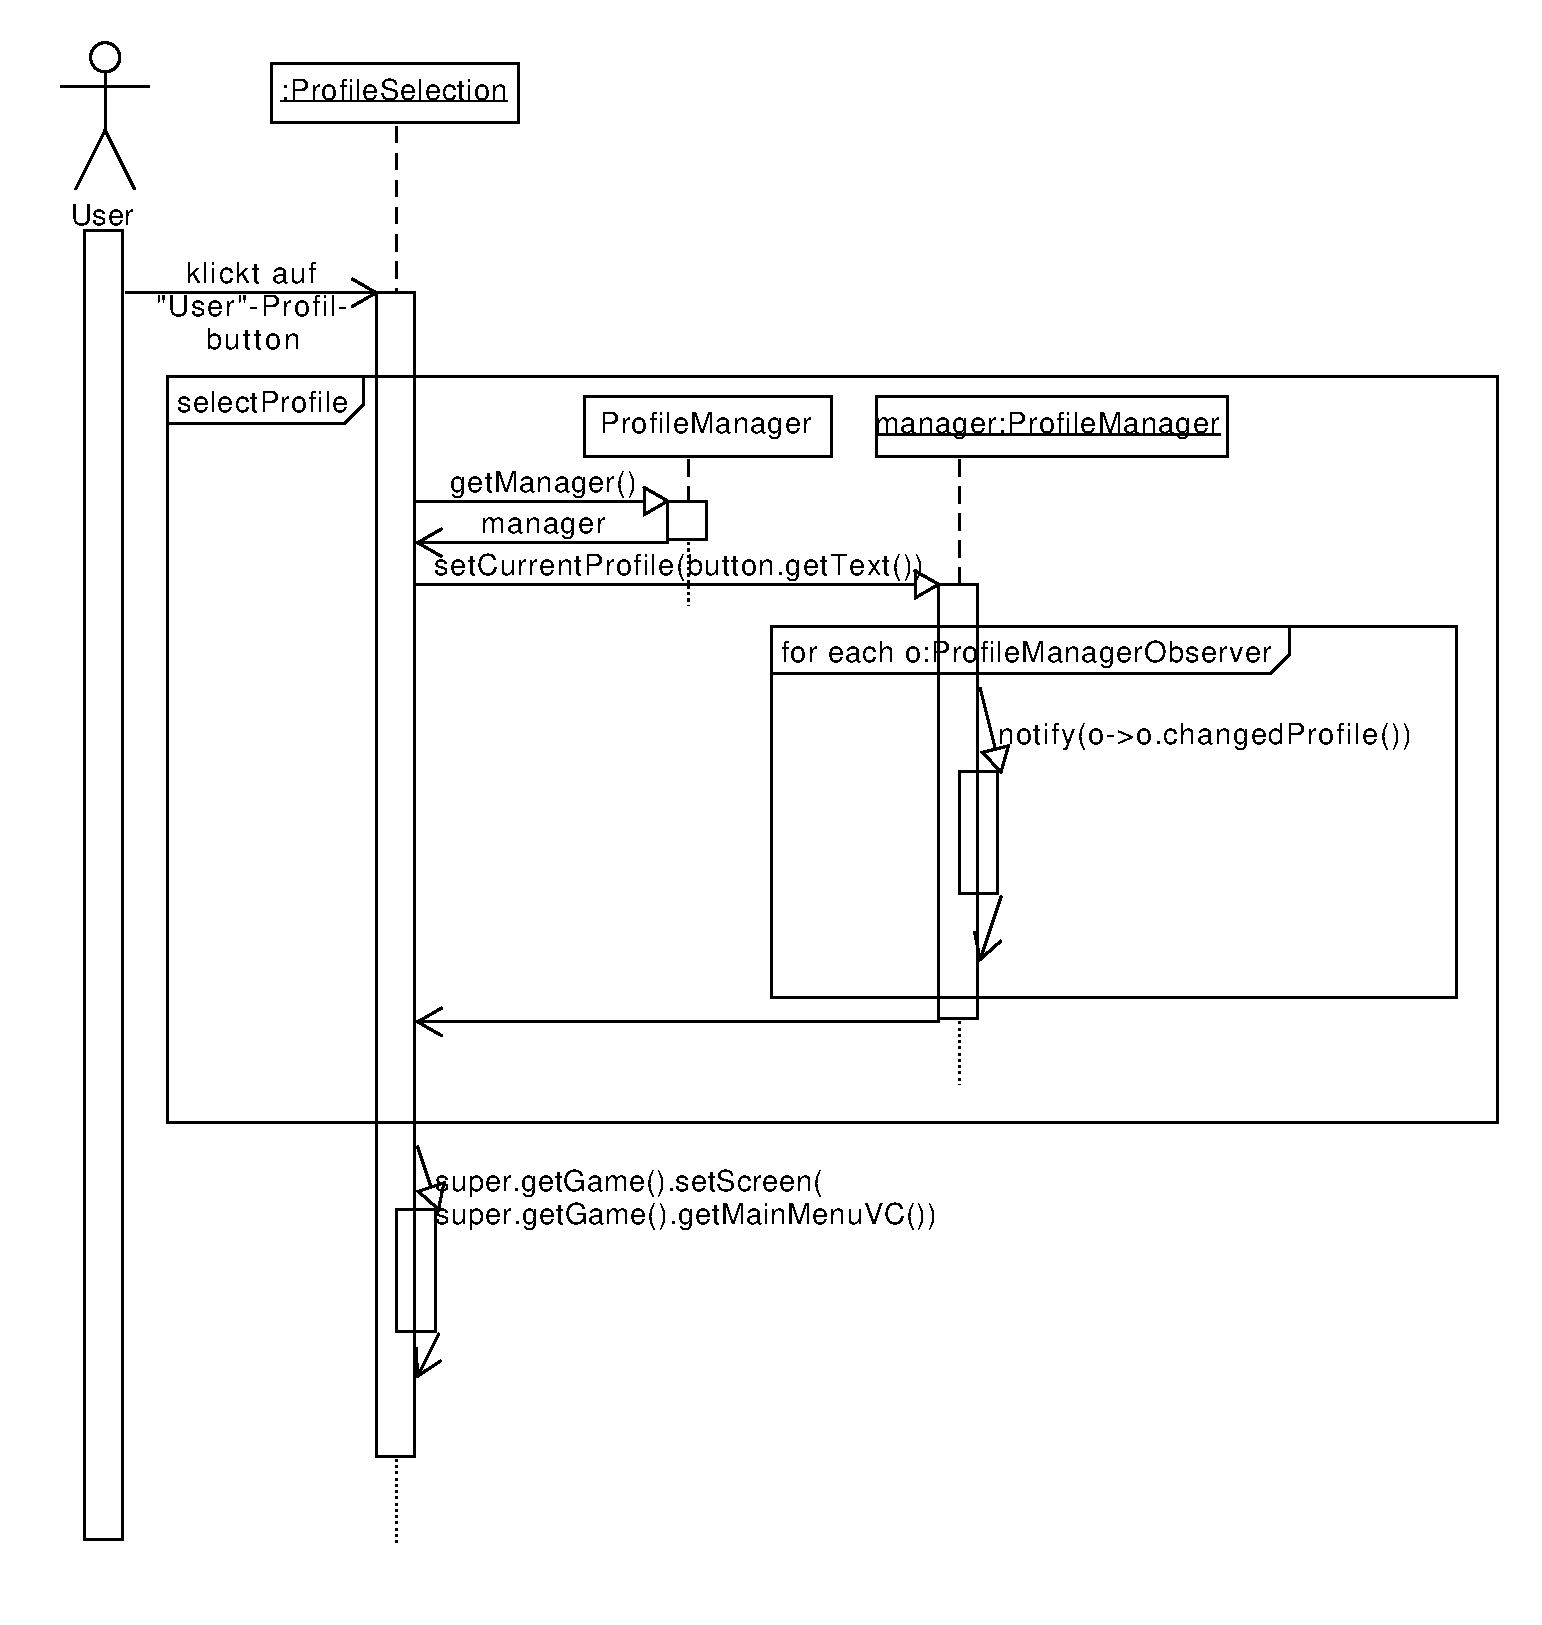
\includegraphics[scale=0.55]{./sections/sequence_diagrams/profile_scenarios/Profilauswahl.pdf}}
\caption{Sequenzdiagramm zur Profilauswahl entsprechend globalem Testfall /T120/ im Pflichtenheft}
\end{figure}

\subsubsection{Profilbearbeitung}
\begin{figure}[H]
\centering
\fbox{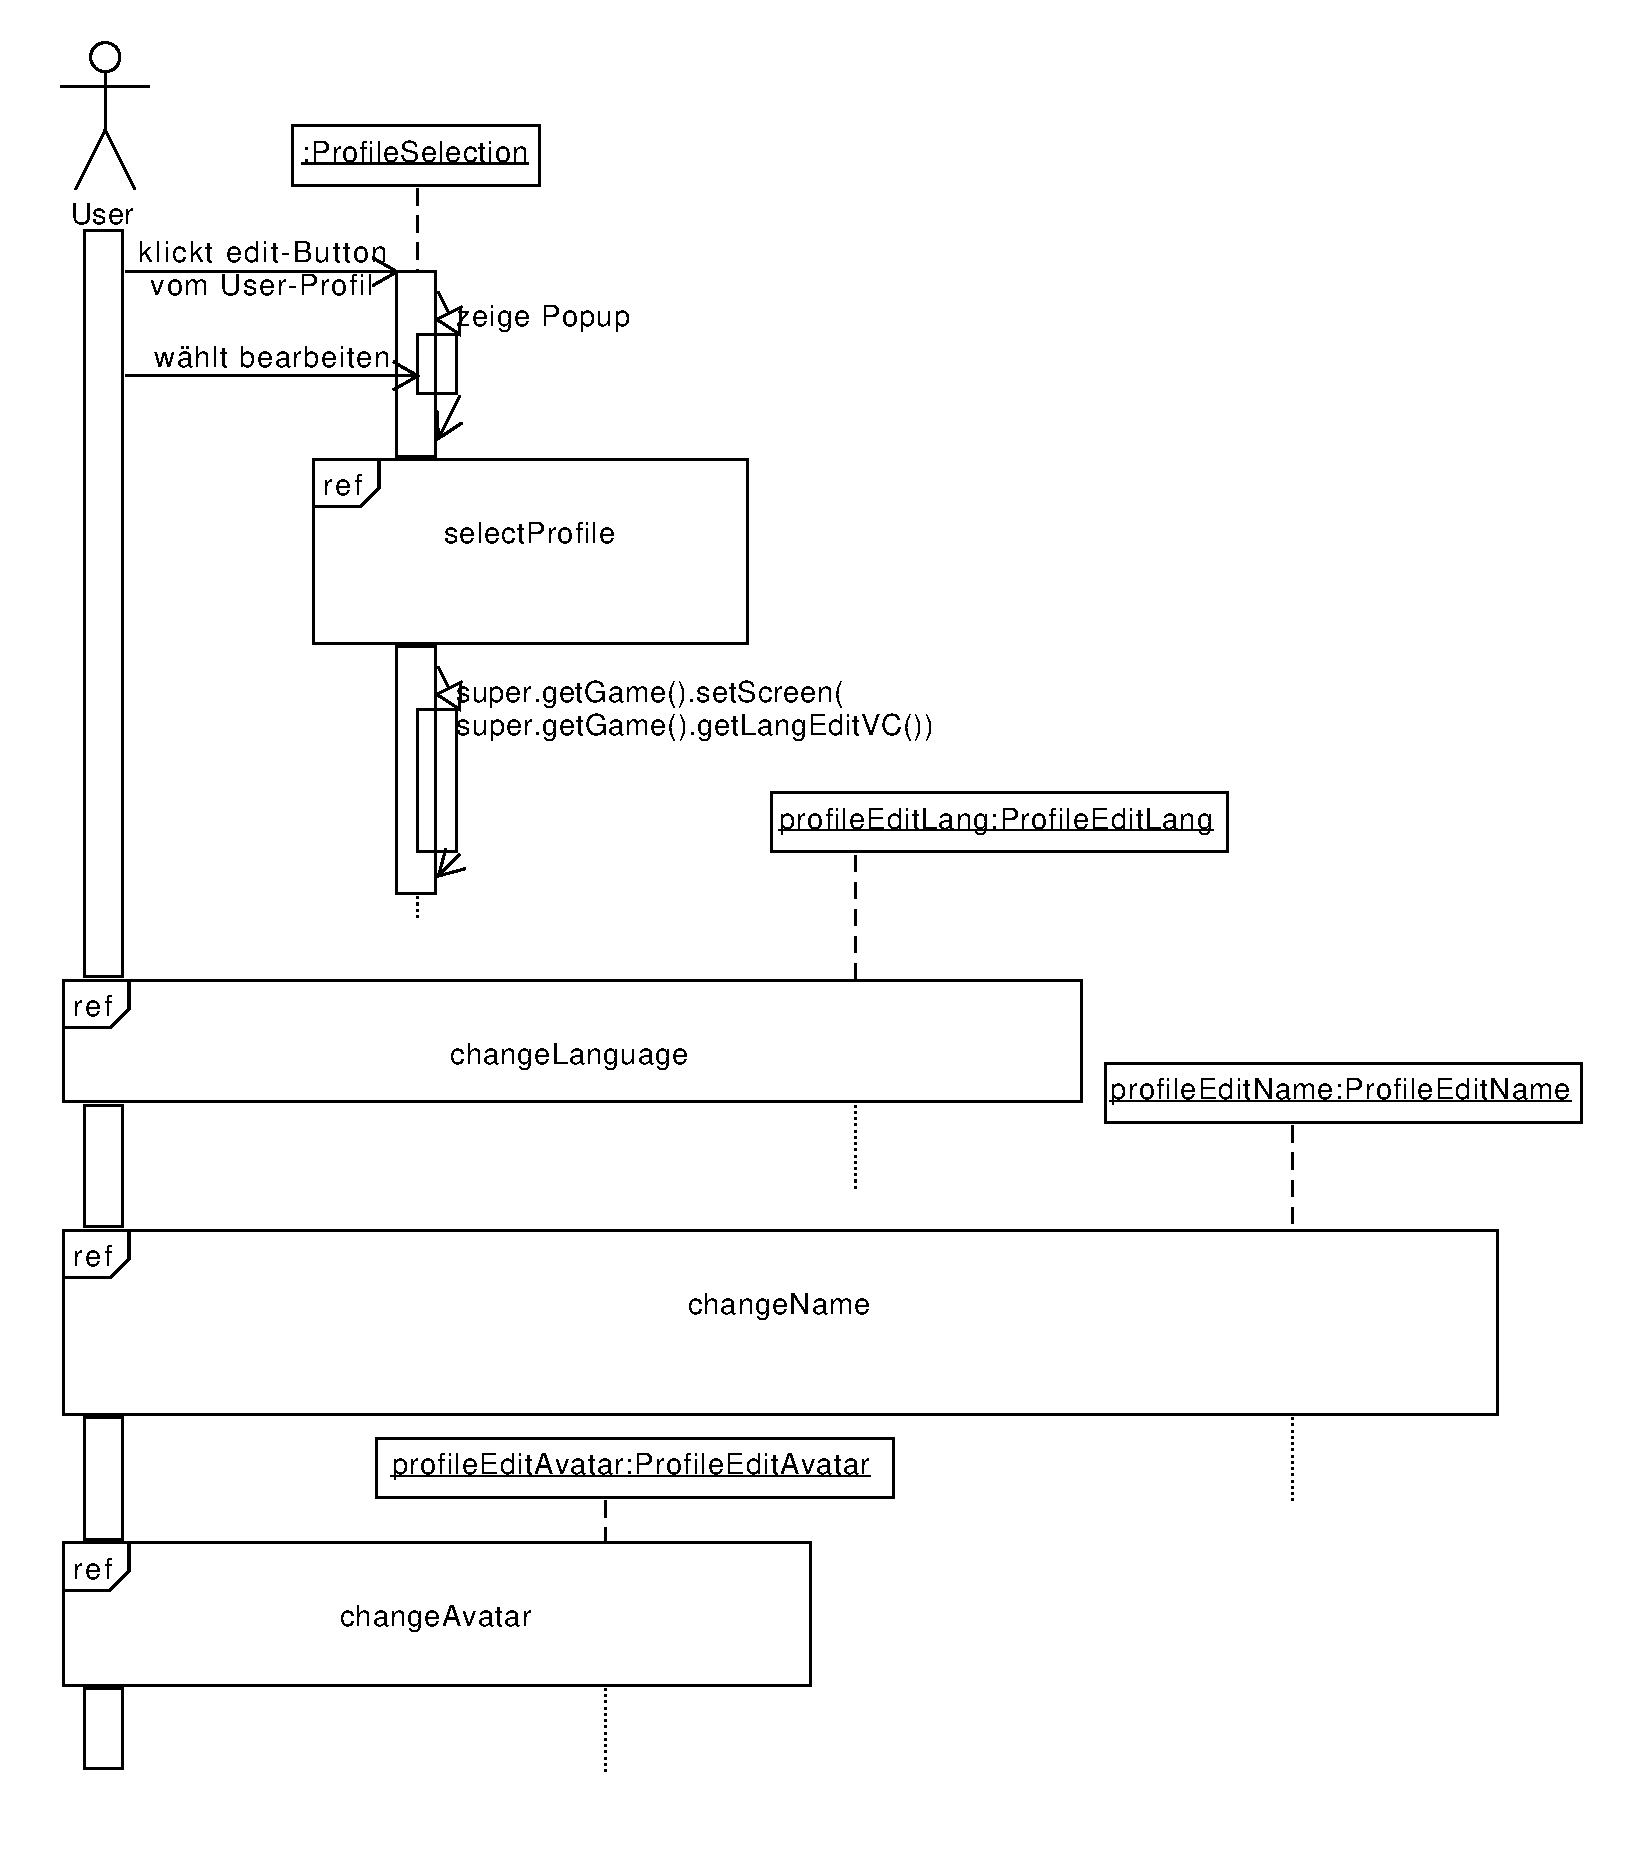
\includegraphics[scale=0.55]{./sections/sequence_diagrams/profile_scenarios/ProfileEdit.pdf}}
\caption{Sequenzdiagramm zur Profilbearbeitung entsprechend globalem Testfall /T130/ im Pflichtenheft}
\end{figure}

\subsubsection{Sprachänderung}
\begin{figure}[H]
\centering
\fbox{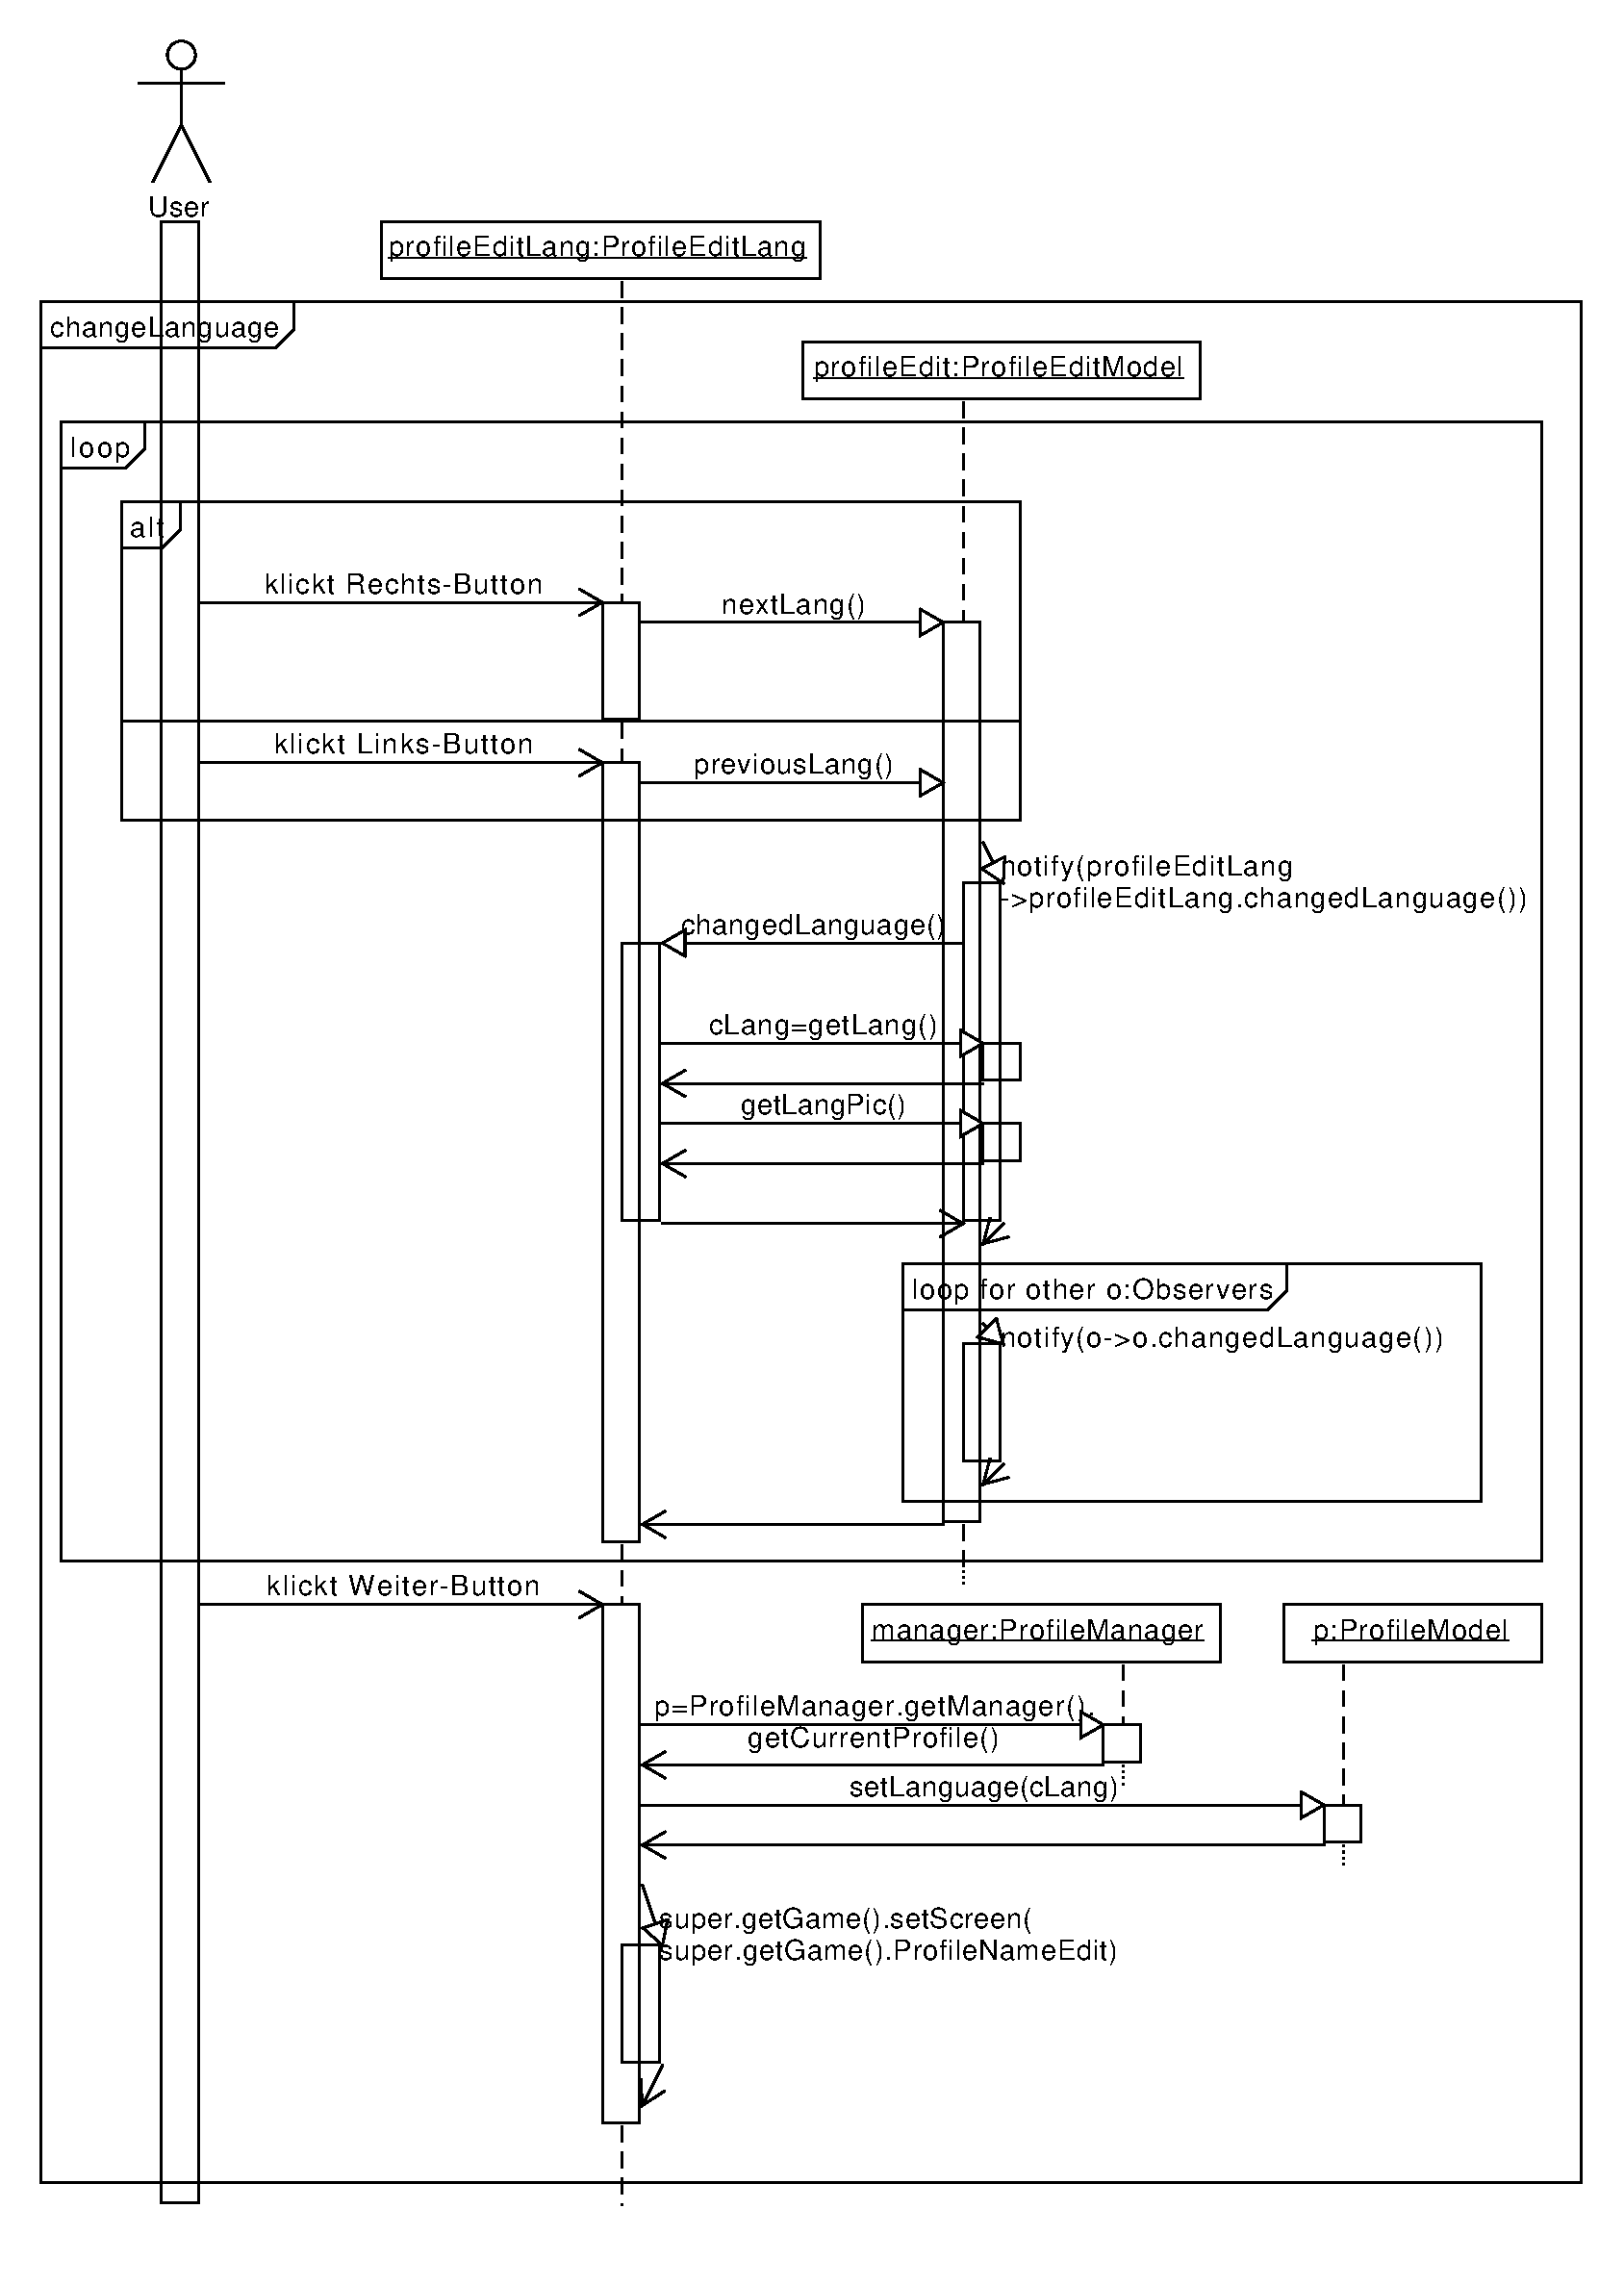
\includegraphics[scale=0.45]{./sections/sequence_diagrams/profile_scenarios/ProfileSprachauswahl.pdf}}
\caption{Sequenzdiagramm zur Sprachänderung}
\end{figure}

\subsubsection{Namenswahl}
\begin{figure}[H]
\centering
\fbox{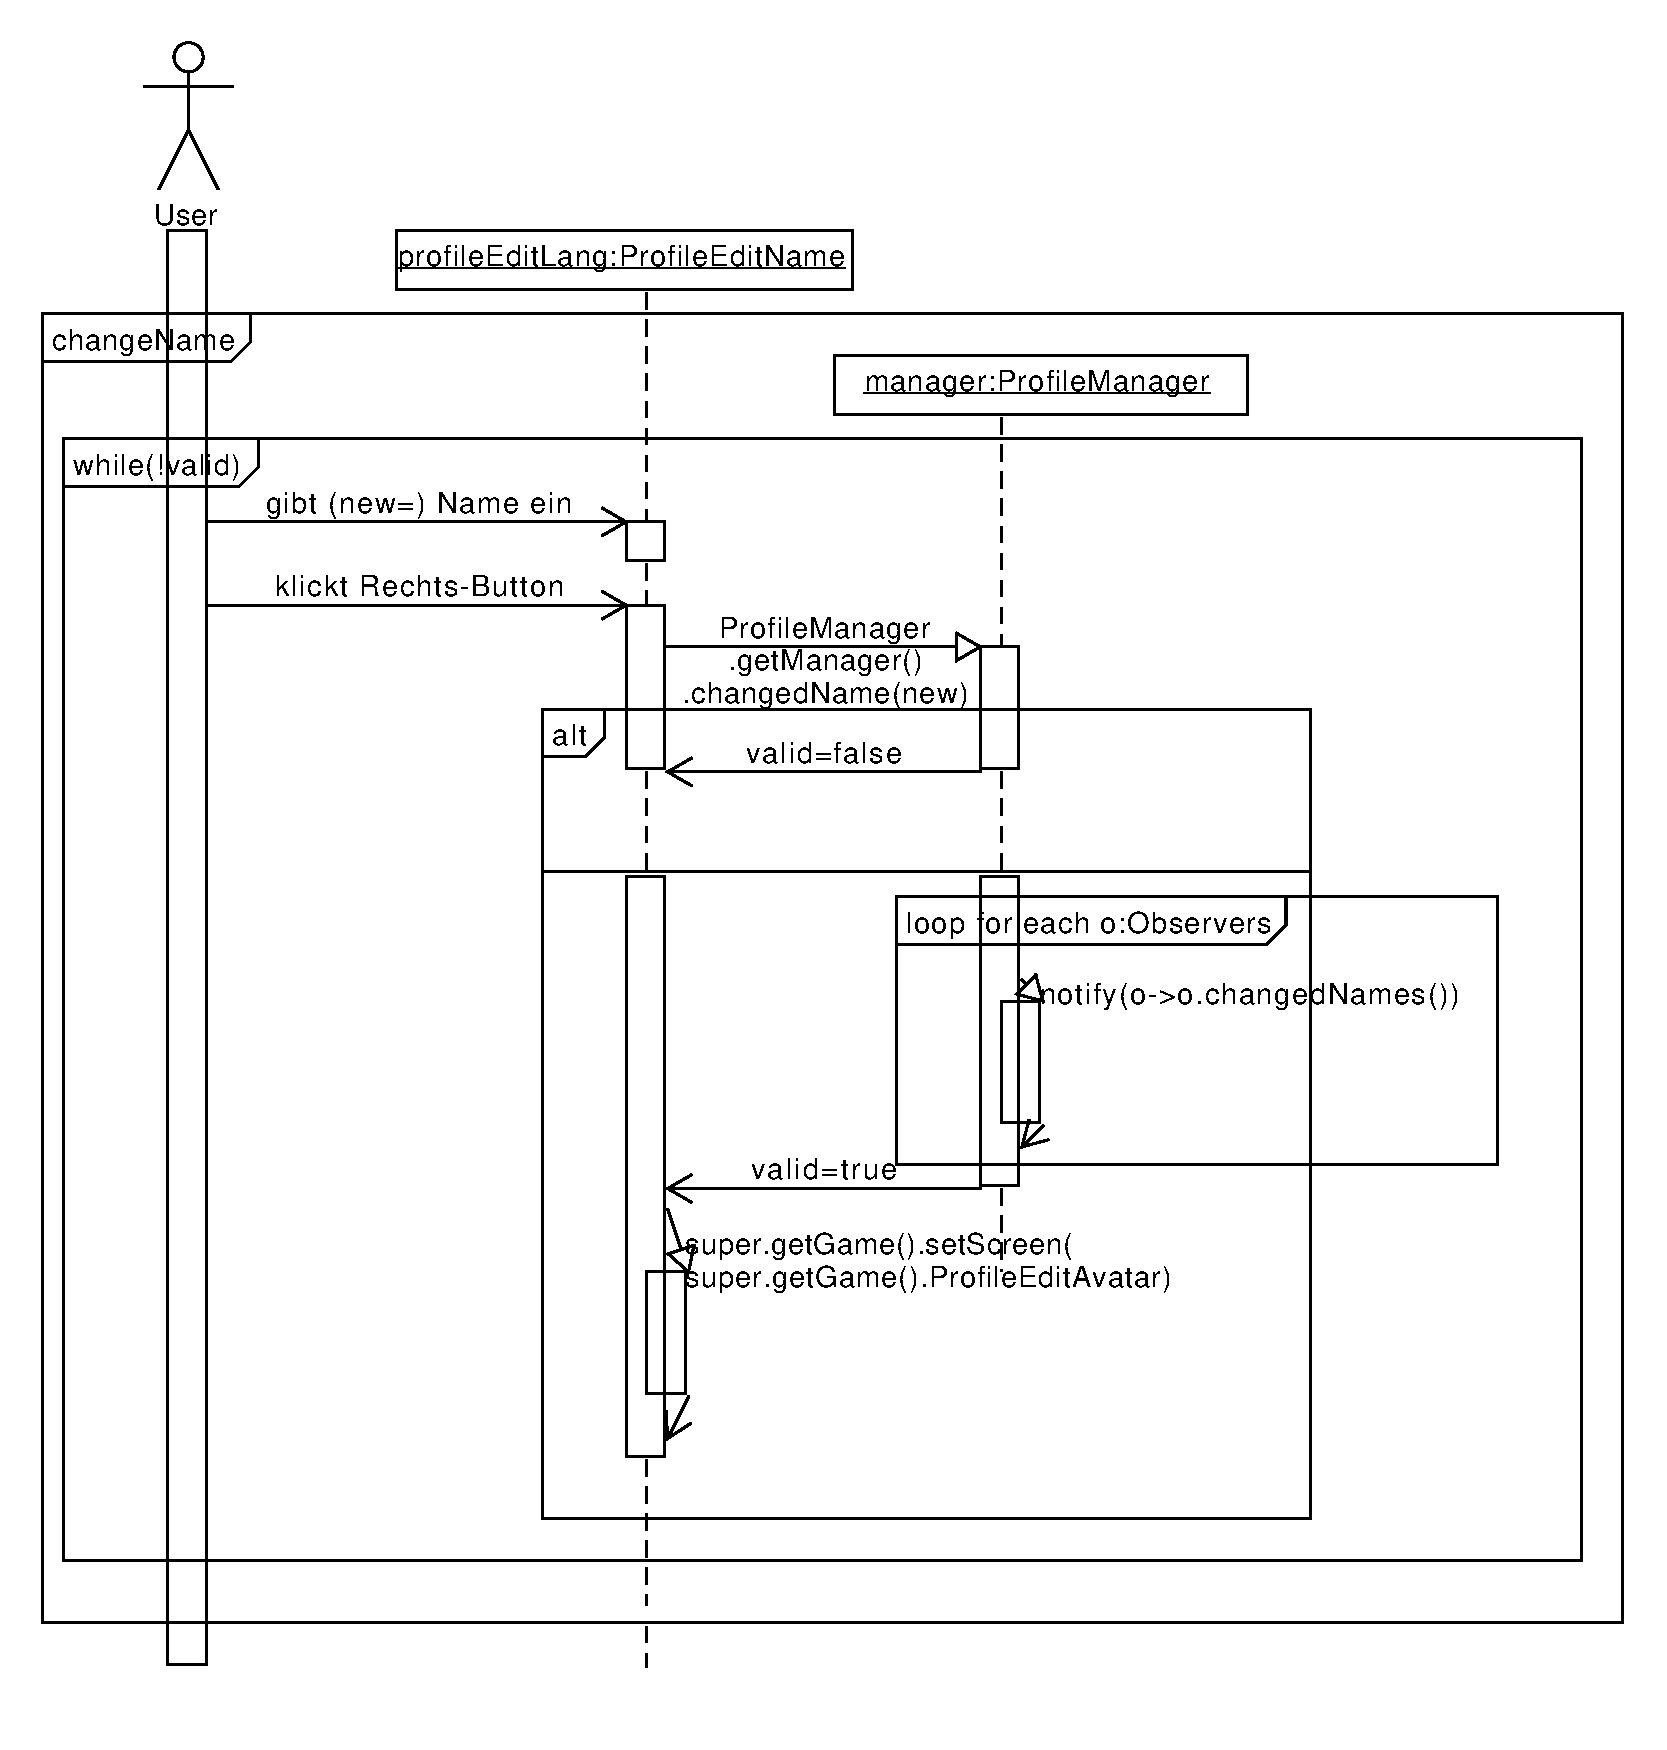
\includegraphics[scale=0.60]{./sections/sequence_diagrams/profile_scenarios/ProfileNamenswahl.pdf}}
\caption{Sequenzdiagramm zur Namenswahl}
\end{figure}

\subsubsection{Avatarauswahl}
\begin{figure}[H]
\centering
\fbox{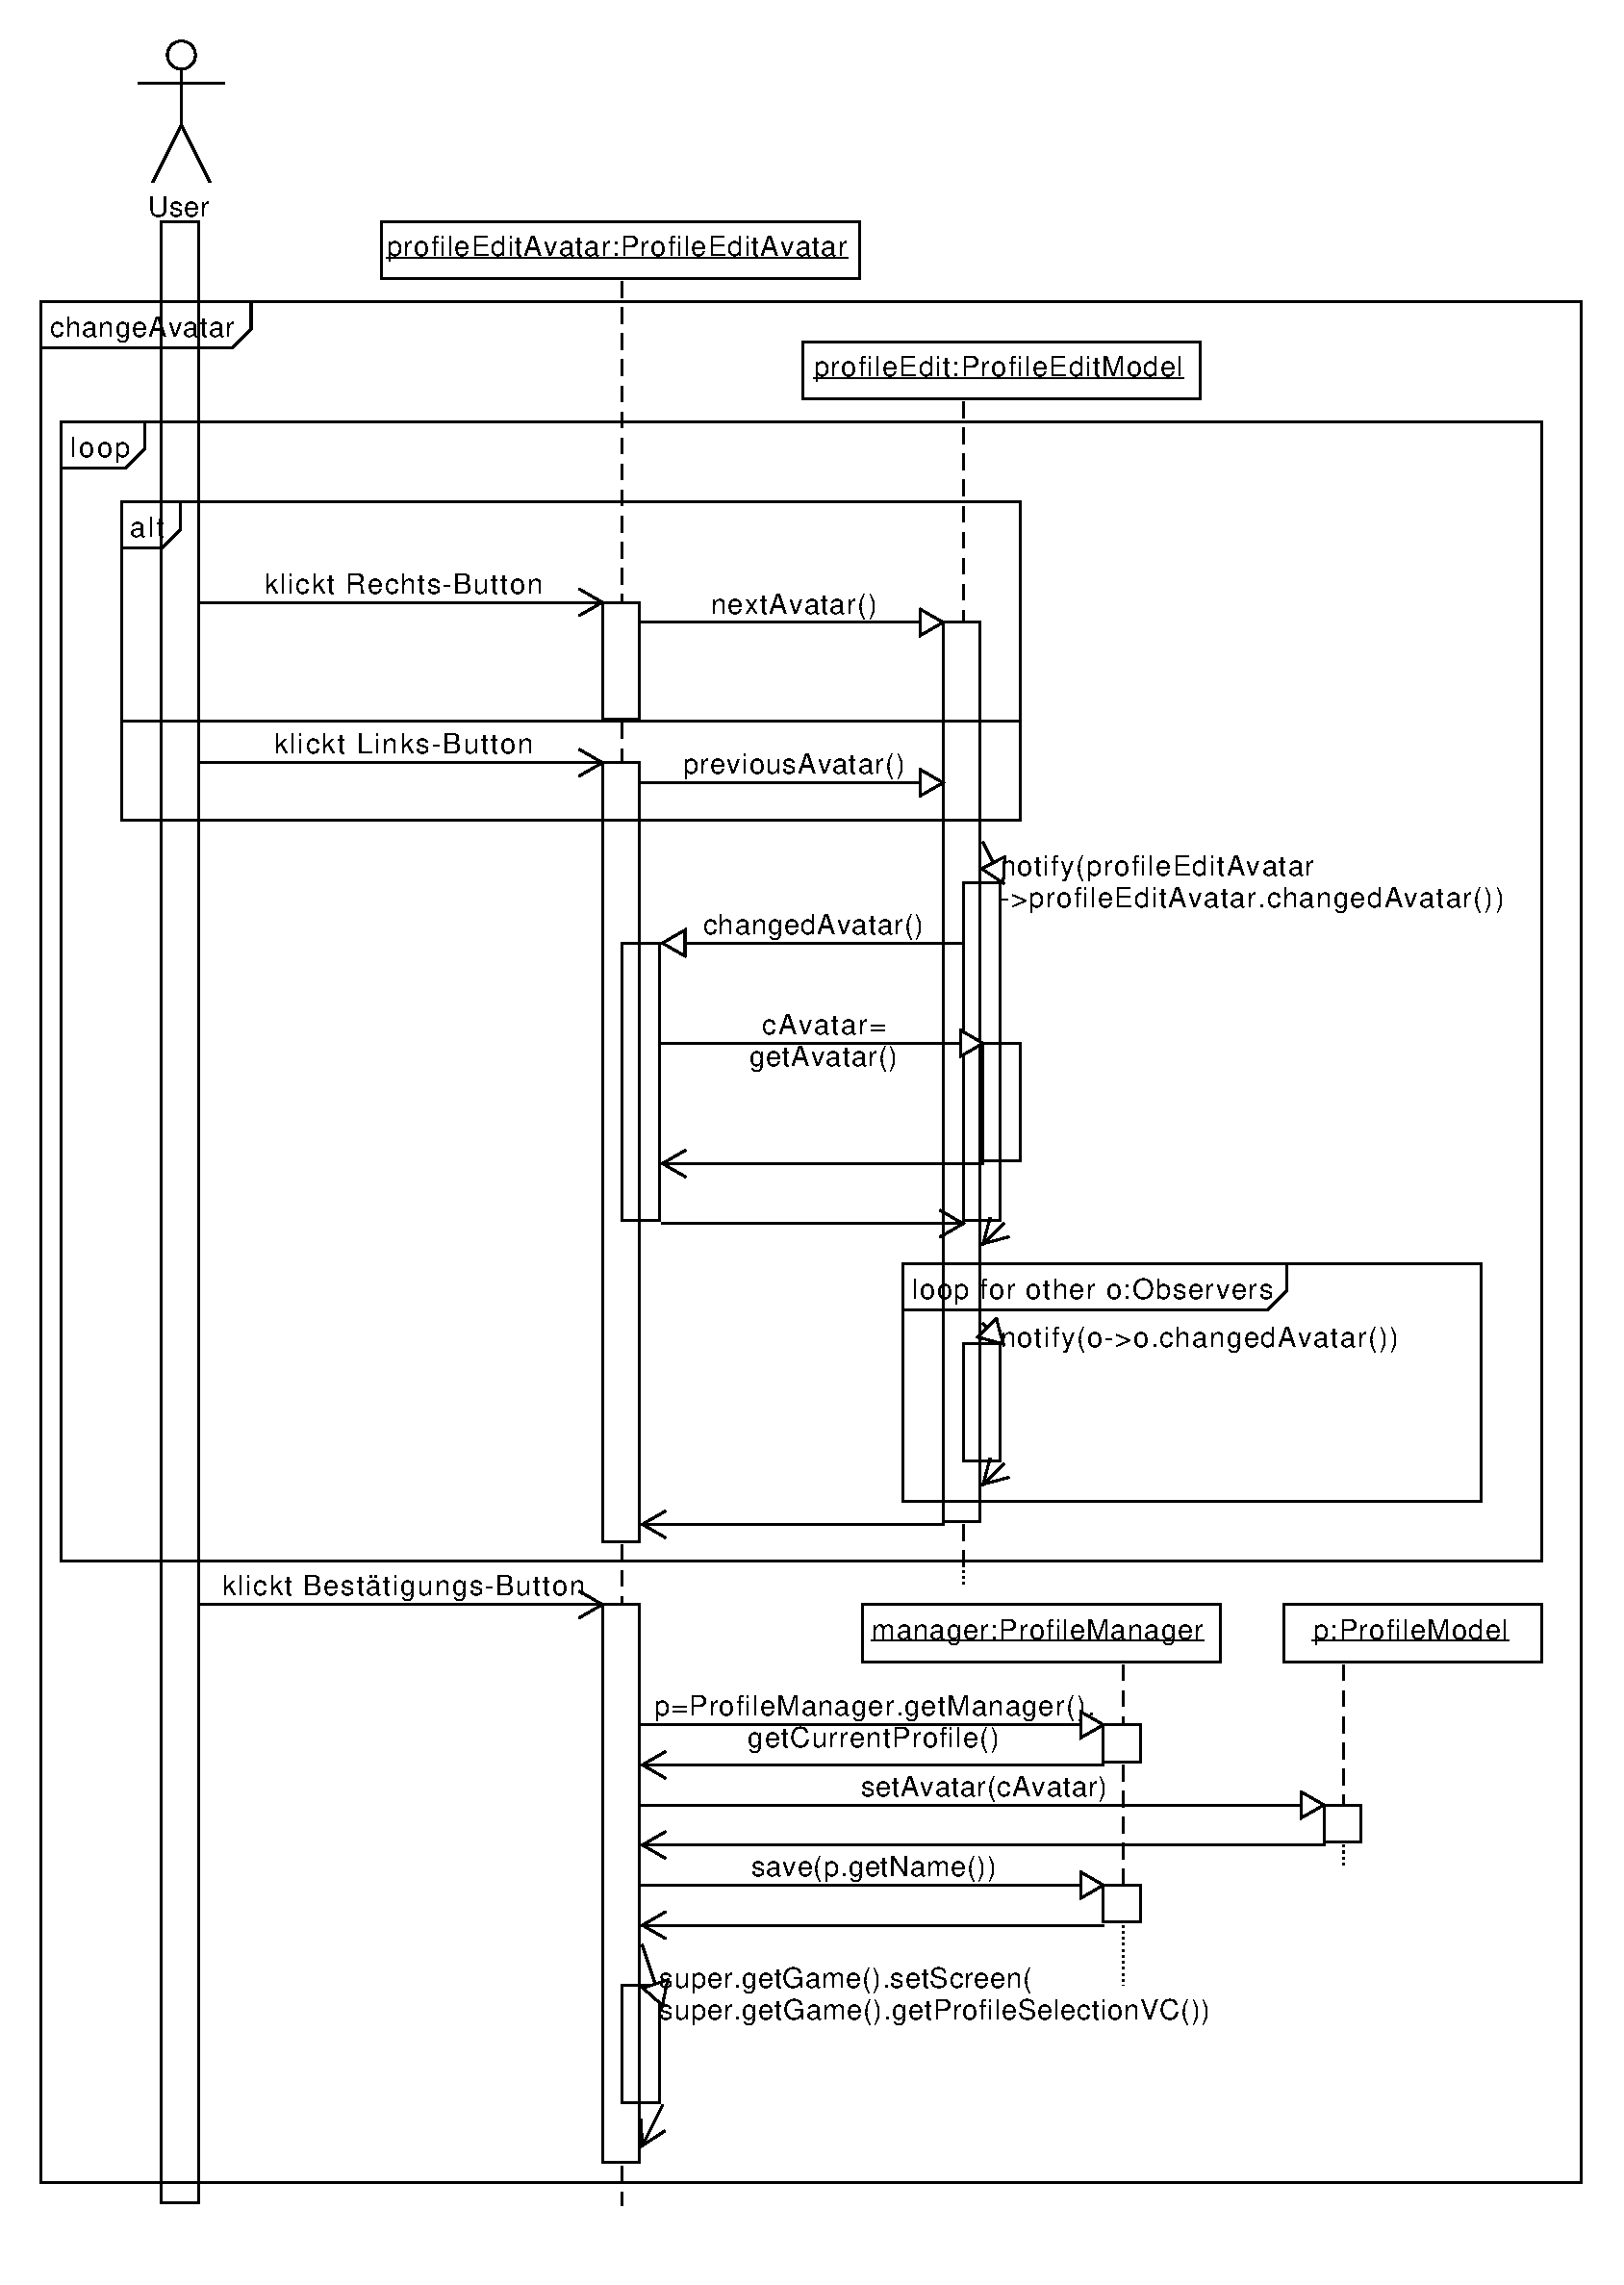
\includegraphics[scale=0.45]{./sections/sequence_diagrams/profile_scenarios/ProfileAvatarauswahl.pdf}}
\caption{Sequenzdiagramm zur Avatarauswahl}
\end{figure}
	\newpage
	\section{Glossar}

	\newpage
	\section{Anhang}


\end{document}